\documentclass[doktyp=marbeit,fontsize=12pt,sprache=english,hausschrift=true,draft=false]{TUBAFarbeiten}

% packages
\usepackage{abstract}
\usepackage{amsmath}
\usepackage[ngerman]{babel}
\usepackage{bashful}
\usepackage{blindtext}
\usepackage{caption}
\usepackage{capt-of}
\usepackage{calc}
% \usepackage[backend=biber,sortlocale=de_DE_phonebook,sorting=none,natbib=true,doi=false,isbn=false,url=false]{biblatex}
% \usepackage[backend=biber,sorting=none,natbib=true,doi=false,isbn=false,url=false]{biblatex}
% \addbibresource{references.bib}
\usepackage{cite}
\usepackage{draftwatermark}
\SetWatermarkText{Confidential}
\SetWatermarkScale{1}
\SetWatermarkColor[gray]{0.9}

\usepackage{enumitem}
\usepackage[T1]{fontenc}
\usepackage{floatrow} % rows of table and pictures
\usepackage{graphicx}
\usepackage{gensymb}
\usepackage[utf8x]{inputenc}
\usepackage{newunicodechar}
\usepackage{makeidx}
\usepackage{subcaption}
\usepackage{tabu}
\usepackage{spreadtab}
\usepackage{pgfplots}
\usepackage{xcolor}
\usepackage{colortbl}
\usepackage{pifont}

\usepackage{algorithm}
\usepackage{algpseudocode}
\usepackage{listings}

\definecolor{lightgray}{HTML}{CBCBCB}
\definecolor{lightergray}{gray}{0.9}
\newcolumntype{a}{>{\columncolor{lightergray}}c}
\newcolumntype{b}{>{\columncolor{white}}c}

\definecolor{darkgreen}{RGB}{65,117,5}
\definecolor{darkred}{RGB}{208,2,27}

\definecolor{plotblue}{HTML}{4A90E2}
\definecolor{plotorange}{HTML}{F5A623}
\definecolor{plotdarkblue}{HTML}{000FFF}
\definecolor{plotdarkorange}{HTML}{FF5200}

% Images with mathcha.io 
\usepackage{tikz}
\usetikzlibrary{fadings}
\usepackage{mathdots}
\usepackage{yhmath}
\usepackage{cancel}
\usepackage{color}
\usepackage[group-separator={,},group-minimum-digits=4]{siunitx}
\usepackage{array}
\usepackage{multirow}
\usepackage{amssymb}
\usepackage{gensymb}
\usepackage{tabularx}
\usepackage{booktabs}
% Images end

\usepackage{subscript} % tief stellen
\usepackage{setspace}
\renewcommand{\baselinestretch}{1.5}

\usepackage{mathtools}
\newcommand{\colvecxx}[2]{\left(\begin{array}{c} #1 \\ #2 \end{array}\right)}
\newcommand{\colvecxxx}[3]{\left(\begin{array}{c} #1 \\ #2 \\ #3 \end{array}\right)}
\newcommand{\colvech}[3]{\left(\begin{array}{c} #1 \\ #2 \\ #3 \\ 1\end{array}\right)}

\newcommand{\rowvecxx}[2]{\left(\begin{array}{cc} #1 & #2 \end{array}\right)^T}
\newcommand{\rowvecxxx}[3]{\left(\begin{array}{ccc} #1 & #2 & #3 \end{array}\right)^T}

\newcommand{\lnorm}[1]{\lVert#1\rVert}

\DeclareMathOperator{\arctantwo}{arctan2}

\DeclarePairedDelimiter{\ceil}{\lceil}{\rceil}
\DeclarePairedDelimiter{\floor}{\lfloor}{\rfloor}
\DeclarePairedDelimiter{\abs}{\lVert}{\rVert} % definiere absoluten betrag

% https://tex.stackexchange.com/questions/9466/color-underline-a-formula
\def\mathunderline#1#2{\color{#1}\underline{{\color{black}#2}}\color{black}}


\usepackage[acronym,toc]{glossaries}
\glstoctrue%

\newglossary[nlg]{symbols}{nls}{nlo}{Symbol Definition}
\makeglossaries%
\loadglsentries{chapter00/acronyms}
\loadglsentries{chapter00/definitions}
\loadglsentries{chapter00/symbols}

% tubaf zeugs
\TUBAFFakultaet{Faculty of Mathematics and Computer Science}
\TUBAFInstitut{Institute for Computer Science}
\TUBAFLehrstuhl{Professorship for Virtual Reality and Multimedia}
\TUBAFTitel{Post-Processing of Depth Images and Laser Scan Data for Feature-based Pose Estimation}
\TUBAFBetreuer{Prof.\ Dr.\ Bernhard Jung}
\TUBAFKorrektor{M. Sc. Robert Lösch}
\TUBAFAutor[J. Toth]{Jonas Toth}
\TUBAFStudiengang{Master Angewandte Informatik}
\TUBAFMatrikel{57319}
% \TUBAFAnmeldeDatum[2019-09-25]{25. September 2019}
\TUBAFDatum{10. June 2020}


\setcounter{tocdepth}{3}
\setcounter{secnumdepth}{3}

% \makeindex

\usepackage[pdftex, unicode, hidelinks,
            pdfproducer={Latex with hyperref},
            pdfcreator={pdflatex}]{hyperref}
\hypersetup{colorlinks=false,
            citecolor=black,
            filecolor=black,
            linkcolor=black,
            urlcolor=black,
            linktoc=all}


% start the content
\begin{document}

\maketitle
\pagenumbering{roman}
\TUBAFErklaerungsseite%

\begin{abstract}
\noindent
Features --- special identifiable bits of data --- and their recognition between different images play an important role in computer vision to solve tasks like visual odometry, place and object recognition or global localization.
Methods for these areas are established and implemented for common mobile devices and robots.
Even though depth data processing is omnipresent for robotic systems, feature detectors for salient, recognizable segments of such pointclouds are not an established method for reliable and robust localization without prior knowledge.

This work proposes depth image processing steps to utilize feature detectors and descriptors for color images on depth data.
In order to apply the algorithms SIFT, SURF, ORB and AKAZE on depth images, they are converted into derived feature images that encode the local geometry of the measured environment.
Multiple possible transformations of the depth data, from the already proposed Bearing-Angle image to measures of curvature and finally the novel Flexion image are developed, analyzed and evaluated with respect to, among other things, keypoint stability and discrimination potential of the descriptors.
The aspects keypoint count, size, response, the matching distance between true and false positives and additional measures like precision, recall and informedness are determined for four experimental datasets.
They consist of a synthetic scene, a underground mining environment, an office scene and LiDAR scans.
In addition, the impact of filtering the depth data with edge-preserving filters is analyzed on the outcome.

All experiments indicate a consistently better performance of the Flexion image compared to the Bearing-Angle image and proof that SIFT and AKAZE are suitable as feature detectors and descriptors whereas SURF and ORB are not.
This insight is underlined with the computation of a visual odometry benchmark.
The research forms a solid foundation to further develop the use of classical computer vision algorithms on Flexion images to accomplish feature-related tasks with depth data.
\end{abstract}

\newpage
\begin{abstract}
Sehr wichtige Arbeit
\end{abstract}

\newpage

\tableofcontents
\newpage

\setlength{\glsdescwidth}{0.82\linewidth}
\setlength{\glspagelistwidth}{0.18\linewidth}
\printglossary[type=\acronymtype,style=super,nonumberlist]%
\newpage

\printglossary
\newpage

\printglossary[type=symbols,style=super]%
\glsaddallunused[symbols]
\newpage


\pagenumbering{arabic}
\newpage

\section{Introduction}\label{sec:introduction}
\subsection{Motivation}

\begin{itemize}
    \item multiple sensors per robot resulting in multimodal sensor fusion requirements
    \item depth sensors increasingly used in the field and quality of sensors improve dramatically
    \item performance/compute costs of ICP high
    \item other approaches require many compuations as well, parallelization is major concern for improving performance
    \item due to ICP limitations, combining laserscan and depth sensor hard
    \item ICP requires correspondent in the pointclouds and inital pose
    \item global positioning not easily done, because of local maxima and computational cost of for example particle based approaches
\end{itemize}

\subsection{Problem Definition}

\begin{itemize}
    \item rigid and non-rigid registration
    \item registering depth and range data
    \item Kinect fusion
    \item dependent on initial pose
    \item some algorithms for laserscan matching work on 2D laser scans, but not dense 3D scans
    \item other multi-modal registrations
    \item mining environment
    \item prior high resolution laser scans exist
    \item bad lighting conditions
\end{itemize}

\subsection{Other Approach}

\begin{itemize}
    \item Scaramuzza\cite{Scaramuzza2007} presented work on registering a camera to a laserscaner using manually selected features in the laserscan and the image
    \item prior conversion of the laserscan to an image dubbed \Glspl{bearing-angle-image}
    \item converted image shows the local geometric structure exposed to the scan

    \item Lin et.al\cite{Lin2017} applied SURF feature detection on \Glspl{bearing-angle-image}
    \item this allows feature based posed estimation with the classical workflow used in SLAM algorithms
\end{itemize}

\subsection{Improvements}

\begin{itemize}
    \item \Glspl{bearing-angle} is calculated in only one direction and can therefore not be rotation invariant
    \item this work proposes \Glspl{flexion-image} that encodes the local geometry in all directions and is rotation invariant
    \item multiple state-of-the-art keypoint detectors and feature descriptors are compared between \Glspl{flexion-image} and \Glspl{bearing-angle-image} on various datasets taken with Kinect v2 and a full Laserscan
    \item evaluation shows better performance of \Glspl{flexion-image} with regard to keypoint quality and feature description
\end{itemize}

\subsection{Structure of this Thesis}


\newpage

\section{Related Work}\label{sec:related_work}
Scaramuzza's work on calibrating the extrinsic of a \acrshort{LIDAR} scanner to a camera\cite{scaramuzza_iros2007} introduces the \gls{bearing-angle-image}.
The conversion of range data to a derived visual representation format allows manual selection of corresponding corners, edges and other salient regions in both the color image and the \gls{bearing-angle-image}\cite{scaramuzza_iros2007}.
Minimizing the reprojection error for the selected points allows to compute a relative rotation and translation between both modalities.
Lin et al.\cite{lin_easp2017} apply the \acrshort{surf}\cite{bay_eccv06} \gls{feature} detector on \glspl{bearing-angle-image} to reconstruct the relative pose between dense pointclouds.
They additionally compare the performance of this registration to state-of-the-art \acrshort{icp} algorithms.
They conclude, that the \acrshort{icp} has higher precision but execution speed is drastically improved when using the \gls{bearing-angle} based pose as initial state.
Zhuang et al.\cite{zhuang_iam2013} apply \acrshort{sift}\cite{lowe_ijcv04} on \glspl{bearing-angle-image} for scene recognition on \acrshort{LIDAR} scans.
To the best of the author's knowledge, no other work includes the use of \glspl{bearing-angle-image}.

\subsection{Pointcloud Registration}

The cited publications are novel approaches to a well researched and developed area --- pointcloud registration.
Range sensors produce a set of points and one natural task is to determine the relative transformation between two such sets.
This task has many applications in photogrammetry, robotics and engineering.

\acrshort{icp}, originally formulated by Besl\cite{besl_pami1992}, is a robust and easy to implement algorithm to achieve this registration.
At its core is the assignment of point correspondences between both sets, calculating a relative pose that results in the lowest distance between the choosen points and evaluating the disparity of both pointclouds.
The mismatch of the pose is iteratively reduced by finding better correspondences using the distance between the points of the pointclouds as error metric.
This basic approach received multiple improvements with generalized \acrshort{icp}\cite{segal_2009,korn_2014} providing a fully probabilistic formulation.
\acrshort{icp} provides a 6 \acrlong{DoF} (\acrshort{DoF}) registration consisting of a rotation and translation.
Convergence or an upper bound of the error is not guaranteed and in general relies on a good initial estimate of the relative pose of both pointclouds, rendering it useless for global registration problems without prior knowledge.
Failure to converge on a relative pose can happen both due to a bad initial pose or not corresponding pointclouds.

A different approach to pointcloud registration is provided by the \acrlong{NDT} (\acrshort{NDT}) algorithm proposed by Biber and Straßer\cite{biber_iros2003}.
It works without explicit correspondences between both pointclouds.
First, the pointcloud is subdivided into cells.
Each cell approximates a normal distribution of the probability of measuring a point at a position within the cell.
Registering a second pointcloud is a matter of maximizing the likelihood that the pointcloud is measured in the reference pointcloud under a given pose.
The normal distributions are differentiable and classical numerical algorithms, like Newton's algorithm, can be used for the maximization.

Myronenko and Song\cite{myronenko_ieee2010} proposed the \acrlong{CPD} (\acrshort{CPD}) algorithm.
Similar to \acrshort{NDT} the algorithm utilizes probabilistic methods to achieve the registration.
A pointcloud is modelled with a \acrlong{GMM} (\acrshort{GMM}) defined through multiple centeroids and their variances.
Again, alignment of two pointclouds means the maximal probability of the data points under the \acrshort{GMM}.
In iterative refinement steps of the relative pose the centeroids of the \acrshort{GMM} are enforced to move in topological consistent fashion, hence coherent point drift.
The review articles~\cite{bellekens_ambient2014,pomerleau_2015} introduce state-of-the-art pointcloud registration algorithms both in general and for robotic applications.
All these methods for pointcloud registration are not suitable to search for a matching segment of a pointcloud or to even select a suitable pointcloud from a database.
For such a task features come into play because they provide a tool to discard unrelated pointclouds fast.

Elbaz et al.\cite{elbaz_cvpr2017} extract subsets of a pointcloud, analyze its main directional components using a principal component analysis and synthesize a depth map for these patches.
A deep neural network based auto-encoder computes a low-dimensional descriptor for each patch.
Registration of pointclouds is achieved by matching these descriptors followed by a conventional fine-tuning step.

Steder et al.\cite{steder_robot2010} proposed an interest point detector for pointclouds.
The image's curvature is analyzed by first smoothing with a Gaussian and then computing the second derivatives of the range data.
High curvature is used for saliency, but special points on edges and regions of occlusion are filtered out first.
Interest points must succeed an empirical found saliency threshold to be selected.
Image based features are suprior in terms of experience in the field, availability and success in a diverse set of use cases\cite{lynen_ros2015,sivic_pami2009,aqel_2016}.

\subsection{Feature Algorithm Comparison}

Keypoint detectors and \gls{feature} descriptors provide a way to detect salient regions of a gray-scale image that can be consistently detected between different views of a scene.
The breakthrough development is Lowe's SIFT\cite{lowe_ijcv04} algorithm.
The early benchmark\cite{mikolajczyk_pami2005} of SIFT to other classical algorithms, like the Harris corner detector\cite{harris_1988}, demonstrated the strong performance of SIFT.
Since the early 2000s more work on improving upon SIFT in terms of performance, compute requirements and diverse applications lead to more competitors like SURF\cite{bay_eccv06}, ORB\cite{rublee_iccv11} and AKAZE\cite{alcantarilla_bmva13}.
A recent comparison between those modern, well established algorithms by Andersson and Reyna Marquez\cite{andersson_2016} still puts SIFT as a top-performer, with AKAZE yielding similar but slightly less accurate results.
ORB\cite{rublee_iccv11} on the other hand is less accurate but due to its lower computational cost still a viable option, especially for mobile applications\cite{andersson_2016}.
The use of classical \gls{feature} descriptors and template based matching for different modalities, like thermal imaging, is evaluated by Gesto-Diaz et al.\cite{gesto-diaz_2017}.
They conclude that the detectors result in many correct matches within on modality.
Correct intermodal matching on the other hand is harder and depends on the modalities used.
They note that combining thermal and depth images yield the worst performance regardless of the used registration technique.
The result is encouraging that algorithms like SIFT\cite{lowe_ijcv04} are not bound to color images but can be used in scenarios with vastly different appearance.
It also motivates the search for better ways to process depth data for \gls{feature}-based matching.

\newpage

\section{Fundamentals}\label{sec:fundamentals}

This section introduces the relevant principles used to create and evaluate the novel approach on depth data processing.

\subsection{Depth Sensors}

Depth sensors play an increasingly important role in modern robotic applications.
They give a robot a fast mean to detect obstacles and locate itself in its environment.
Additionally gathering this information does not require expensive computations as for example stereo triangulation does.

The following paragraphs describe the underlying sensor principles for the depth sensors used in this thesis, but does not introduce the general area of depth sensing.
Technologies like RADAR and Ultrasonic Sensors as well as sensor setups used in different contexts that do not apply to the conditions of this thesis are not considered.

\subsubsection{Structured-Light Depth Sensors}

\begin{figure}[H]
    \centering
    \begin{subfigure}[t]{0.45\textwidth}
        \includegraphics[width=\textwidth]{chapter03/img/depth_pattern_face.png}
        \caption{Structured light depth sensors project a predefined light pattern into the environment and observe the deformation of that pattern\cite{sl_depthsensor_calibration}.}
    \end{subfigure}~
    \begin{subfigure}[t]{0.45\textwidth}
        \includegraphics[width=\textwidth]{chapter03/img/depth_face_reconstructed.png}
        \caption{This figure shows the reconstruction result of the scanned face scanned\cite{sl_depthsensor_calibration}.}
    \end{subfigure}
    \caption[Visible light pattern used for structured-light depth sensors]{One way to reconstruct depth information are structured light depth sensors. A predefined light pattern is projected into space. As the photons reflect from obstacles at different distances relative to the observer, the light pattern appears transformed. This deformation is used to reconstruct the geometry of the objects. The light emitted is usually not visible to humans as infrared light sources and cameras are commonly used in robotic applications.\label{fig:sl_face}}
\end{figure}

\begin{itemize}
    \item commonly found depth sensor in robotic applications
    \item most notable kinectv1 is a structured light sensors
    \item project grid structure in the world with infrared light
    \item sense the deformation of the grid lines and calculate the distance of an object from this deformation
    \item because the whole scene is captured at once, SL sensor operate at real time frame rates
\end{itemize}

\subsubsection{\acrlong{ToF}-Cameras}

\begin{figure}[H]
    \centering
    \begin{subfigure}[t]{0.45\textwidth}
        \includegraphics[width=\textwidth]{chapter03/img/tof_traveltime_original.png}
        \caption{One way to measure the time-of-flight for photons is to emit a light pulse and measure the roundtrip time until sensing. Illustration adopted from\cite{tof_cameras}.}
    \end{subfigure}~
    \begin{subfigure}[t]{0.45\textwidth}
        \includegraphics[width=\textwidth]{chapter03/img/tof_phase_shift_original.png}
        \caption{The second, more recent approach is measuring the phase-shift of photons relative to the light source. This allows a continously emitting light source. Illustration adopted from\cite{tof_cameras}.}
    \end{subfigure}
    \caption[Illustration of two commonly used measuring principle for Time-of-Flight cameras]{Measuring the distance of objects via time-of-flight\label{fig:tof_illustration}}
\end{figure}

\begin{itemize}
    \item range imaging camera system to measure the distance of world point by measuring the time, light needs to travel to the object and back for every pixel of an image
    \item the light source can be a laser or a LED
    \item the technology is related to \acrshort{LIDAR}
    \item these camera systems operate faster than \acrshort{LIDAR} but have lower resolution
    \item especially in robotics the kinect v2 is commonly found as time-of-flight sensor
    \item phase-shift reduces range of measurement to a few meters, depending on the wavelength of the used light
\end{itemize}

\subsubsection{\acrlong{LIDAR}}

\acrlong{LIDAR} (\acrshort{LIDAR}) uses the same measurement principle as \acrshort{ToF}-Cameras, it measures the distance of an object using time measurements.
The difference between \acrshort{LIDAR} and \acrshort{ToF}-Cameras is the usage of a \acrshort{laser} as light source.
The most common configurations use a horizontally rotating mirror that reflects the beam into the room.
For vertical coverage measurement head is rotated in total.
Each complete horizontal measurement is called a scan line.
This setup allows for different levels of precision and speed.

Some \acrshort{LIDAR}, especially mobile systems with real time requirements, measure in the order of magnitude $10^1$ number of scan lines.
Such systems achieve a higher framerate, but are not considered in this thesis.
For the choosen feature-based approach a dense \acrshort{LIDAR} scan is required.
Such scans can be created with terrestrial lidar stations, common in geodesic applications.
Additionally an intensitiy value can be measured by the light sensors that corresponds to the level of absoption of the reflecting surface.

Flash \acrshort{LIDAR} is a scannerless type of \acrshort{LIDAR} that does not require a rotating mirror or other mechanical system.
These sensors can measure an entire scene in one shot.
A flash \acrshort{LIDAR} is similar to a \acrshort{ToF}-camera and measures a dense range image.
% TODO cite 10.1109/SSIAI.2010.5483929

\begin{itemize}
    \item light detection and ranging
    \item measure the time a laser beam requires travels to an obstacle
    \item reflected light is analyzed, both phase shift and time of travel give information about distance
    \item intensity can be measured by some laser scanners as well
    \item broad spectrum of application in various disciplines
    \item can be full resolution 3D scanning or provide vertically sparse scan lines
    \item in this work dense laser scans are of interest
\end{itemize}

\subsubsection{Depth Sensors used in Experiments}

\begin{table}
\begin{tabular}{l|l|l}
    Sensor & Type & Result Properties \\
    \hline
    KinectV1 & Structured-Light-Camera & Resolution: $320 \times 240$ px \\
    KinectV2 & \acrshort{ToF}-Camera & Resolution: $512 \times 424$ px \\
    Intel Realsense & Structured-Light-Camera & Resolution: $512 \times 424$ px \\
    % TODO: Welches LIDAR haben die Geodäten?
    LIDAR RIEGL VZ-400i & terrestrial \acrshort{LIDAR} & Resolution: $512 \times 424$ px \\
    \caption[List of tested depth sensors]{This table lists all depth sensors that are tested during the master thesis. Not all of them give in usable results for the intended feature-based registration.}
\end{tabular}
\end{table}

\subsection{Coordinate Systems}

This section introduces the used coordinates systems and naming conventions that model the sensory system commonly used in computer vision.
Additionally, homogeneous coordinates allow efficient computation of rotation and translation with one matrix-vector multiplication and knowledge of it is a prerequisite.
Both~\cite{hartley_2004} and~\cite{corke_2011} provide excellent coverage of these topics.

\subsubsection*{Naming Conventions}

A point in space is referenced by a vector in that space.
The global reference frame is arbitrarily choosen in \emph{world coordinates}.
Within that world coordinate system exist one or more sensors spanning their own coordinate system.
Referencing the point relative to such a sensor yields \emph{camera coordinates}.
The sensor itself performs some form of dimension reducing projection of the three dimensional point to a two dimensional point, an \emph{image coordinate}.
\emph{Image coordinates} are an intermediate representation before discretizing the point to individual pixels, called \emph{pixel coordinates}.
Inverting this projection results in \emph{spherical coordinates}, camera coordinates with unit length that just encode the direction of a light ray that hits a pixel.
Different sensor models describe these projecting transformations mathematically.
Note, that the relative transformation between \emph{camera coordiantes} and \emph{world coordinates}, the sensors \emph{pose}, can change over time.
Multiple sensors can exist within the \emph{world coordinate system}.

\subsubsection*{Coordinate Transformations and Pose}

\begin{figure}[H]
    \scalebox{0.7}{%
    \tikzset{every picture/.style={line width=0.75pt}} %set default line width to 0.75pt        

\begin{tikzpicture}[x=0.75pt,y=0.75pt,yscale=-1,xscale=1, style={font=\boldmath}]
%uncomment if require: \path (0,300); %set diagram left start at 0, and has height of 300

%Shape: Circle [id:dp39370051291999986] 
\draw  [draw opacity=0][fill={rgb, 255:red, 74; green, 144; blue, 226 }  ,fill opacity=1 ] (152.42,50.67) .. controls (152.42,47.68) and (154.84,45.25) .. (157.83,45.25) .. controls (160.82,45.25) and (163.25,47.68) .. (163.25,50.67) .. controls (163.25,53.66) and (160.82,56.08) .. (157.83,56.08) .. controls (154.84,56.08) and (152.42,53.66) .. (152.42,50.67) -- cycle ;
%Shape: Axis 2D [id:dp7479977699053467] 
\draw [line width=1.5]  (23,272.35) -- (338.83,272.35)(23,9) -- (23,272.35) -- cycle (331.83,267.35) -- (338.83,272.35) -- (331.83,277.35) (18,16) -- (23,9) -- (28,16)  ;
%Shape: Axis 2D [id:dp43513516367104466] 
\draw [line width=1.5]  (313.19,230.01) -- (380.96,36.17)(114.83,160.67) -- (313.19,230.01) -- cycle (373.93,41.13) -- (380.96,36.17) -- (383.37,44.43) (119.79,167.7) -- (114.83,160.67) -- (123.09,158.26)  ;
%Straight Lines [id:da8557794245884446] 
\draw [color={rgb, 255:red, 74; green, 74; blue, 74 }  ,draw opacity=1 ]   (23,272.35) -- (156.27,53.23) ;
\draw [shift={(157.83,50.67)}, rotate = 481.31] [fill={rgb, 255:red, 74; green, 74; blue, 74 }  ,fill opacity=1 ][line width=0.08]  [draw opacity=0] (8.93,-4.29) -- (0,0) -- (8.93,4.29) -- cycle    ;
%Straight Lines [id:da7386423573093532] 
\draw [color={rgb, 255:red, 74; green, 74; blue, 74 }  ,draw opacity=1 ]   (23,272.35) -- (310.22,230.45) ;
\draw [shift={(313.19,230.01)}, rotate = 531.7] [fill={rgb, 255:red, 74; green, 74; blue, 74 }  ,fill opacity=1 ][line width=0.08]  [draw opacity=0] (8.93,-4.29) -- (0,0) -- (8.93,4.29) -- cycle    ;
%Straight Lines [id:da6638828901158511] 
\draw [color={rgb, 255:red, 74; green, 74; blue, 74 }  ,draw opacity=1 ]   (313.19,230.01) -- (159.8,52.93) ;
\draw [shift={(157.83,50.67)}, rotate = 409.1] [fill={rgb, 255:red, 74; green, 74; blue, 74 }  ,fill opacity=1 ][line width=0.08]  [draw opacity=0] (8.93,-4.29) -- (0,0) -- (8.93,4.29) -- cycle    ;

% Text Node
\draw (153,26) node [anchor=north west][inner sep=0.75pt]  [color={rgb, 255:red, 74; green, 144; blue, 226 }  ,opacity=1 ] [align=left] {$\displaystyle \mathbf{P}$};
% Text Node
\draw (73,134) node [anchor=north west][inner sep=0.75pt]   [align=left] {$\displaystyle \vec{P}$};
% Text Node
\draw (11,280) node [anchor=north west][inner sep=0.75pt]   [align=left] {$\displaystyle O$};
% Text Node
\draw (309.19,237.01) node [anchor=north west][inner sep=0.75pt]   [align=left] {$\displaystyle C$};
% Text Node
\draw (242,117) node [anchor=north west][inner sep=0.75pt]   [align=left] {$\displaystyle \vec{P'}$};
% Text Node
\draw (142,231) node [anchor=north west][inner sep=0.75pt]   [align=left] {$\displaystyle H$};


\end{tikzpicture}

    }
    \caption[Coordinate transformation]{\emph{Coordinate transformation.} Relationship between different representation of the same point in different coordinate systems. The relationship displayed here and the corresponding linear algebra holds true for cartesian coordinate systems of any dimension.}
\end{figure}

Let $\mathbf{O_\mathcal{W}}$ be the origin of the \emph{world coordinate system}.
A three dimensional vector $\vec{P_\mathcal{W}} = \rowvecxxx{U}{V}{W}$ represents a point in this room relative to the origin $\mathbf{O_\mathcal{W}}$.
Seeing this point $\mathbf{P_\mathcal{W}}$ from a camera $\mathbf{C_\mathcal{W}}$ within the same room is equivalent to changing the coordinate system from \emph{world coordinates} to \emph{camera coordinates} of that sensor.
The relative rotation and translation of the camera $\mathbf{C_\mathcal{W}}$ to the room is also called its \emph{pose}.
It is parametrized by a rotation matrix $R$ and a translation vector $\vec{t}$.
Homogeneous coordinates provide a computational more efficient way to apply the transformation to vectors by $4 \times 4$ matrix-vector multiplication instead of $3 \times 3$ matrix-vector multiplication and an additional $3 \times 1$ vector addition.
The point $\mathbf{P_\mathcal{W}}$ seen from the camera $\mathbf{C_\mathcal{W}}$ is computed with the homogeneous transformation matrix $H = \begin{bmatrix} R & \vec{t} \\
    \begin{matrix}0 & 0 & 0\end{matrix} & 1 \end{bmatrix}$.
\begin{equation}
\begin{aligned}
    \colvech{X}{Y}{Z}&= \begin{pmatrix}
        r_{11} & r_{12} & r_{13} & t_x \\
        r_{21} & r_{22} & r_{23} & t_y \\
        r_{31} & r_{32} & r_{33} & t_z \\
        0      & 0      & 0      & 1 \\
    \end{pmatrix} \colvech{U}{V}{W} \\
    \vec{P_\mathcal{C}} &= H \vec{P_\mathcal{W}}
\end{aligned}
\end{equation}
Coordinate transformations do not loose information.

\subsection{Image Formation and Camera Models}

Each depth sensors measurement returns a matrix with depth or range values.
The projection model of the sensor performs the calculation of the camera coordinates for each point.
Additionally, sensor usually experience some form of imperfection in the imaging process, like lense distortion or misalignment of components.
These imperfections are corrected with additional models, like the distortion model for pinhole cameras.

Both calibration and error correction are out of the scope of this thesis and sensor input is expected to adhere to the basic models.
This might require preprocessing of the raw sensor data.
On robotic platforms like \acrlong{ROS} this is done automatically when providing a matching calibration of the sensor.

\subsubsection{Pinhole Camera Model}

The pinhole camera model is the most common camera model in computer vision modelling both classical and depth cameras.

\begin{figure}[H]
    \includegraphics[width=0.6\textwidth]{chapter03/img/pinhole_camera_model.png}
    \caption[Pinhole Camera Model]{The pinhole camera model performs the perspective projection of three dimensional points into the plane. Real cameras additionally have a lense system that can result in radial and tangential distortion. These effects must be componsenated with a proper calibration of distortion models. The camera-coordinate-to-pixel-coordinate projection looses information on the depth. Therefore, the back projection results only in the direction of the light ray. The depth sensor gives the additional distance information to recover the point in camera coordinates. Graphic adopted from\cite{opencv_pinhole}.}\label{fig:pinhole_model}
\end{figure}
Figure~\ref{fig:pinhole_model} shows the perspective projection of three-dimensional points onto the plane.
This projection reduces the input dimension by one and is not depth preserving.

The model is parameterized by the focal length $f_x$ and $f_y$ that correspond to the distance of the pinhole to the image plane, the skew $s$ that resembles non-quadratic pixel shape and is most of the time $s = 0$ and the image center $c_x$ and $c_y$.

\subsubsection*{Forward Projection}

Let $\vec{P} = \rowvecxxx{X}{Y}{Z}$ be a world point in camera coordinates.
The perspective projection
\begin{equation}
    \vec{\hat{p}} = \colvecxxx{x}{y}{1} = \frac{1}{Z}\colvecxxx{X}{Y}{Z}
    \label{eq:pinhole_forward}
\end{equation}
results in the point $\vec{P}$ in image coordinates $\vec{\hat{p}}$. This step looses the depth information.
The image coordinates could be distorted and any correction would happen at this stage.
Multiplication of the $3 \times 3$ camera matrix $K$ and the homogeneous image coordinates results in the final pixel coordinates.
\begin{equation}
\begin{aligned}
K &= \begin{pmatrix}
        f_x & f_x s & c_x \\
        0   & f_y   & c_y \\
        0   & 0     & 1
     \end{pmatrix} \\
K \vec{\hat{p}} &= \begin{pmatrix}
        f_x & f_x s & c_x \\
        0   & f_y   & c_y \\
        0   & 0     & 1
     \end{pmatrix}\colvecxxx{x}{y}{1} = \colvecxxx{u}{v}{1} = \vec{p}
\end{aligned}
\end{equation}

\subsubsection*{Backward Projection}

Applying the inverse transformations allows to recover the direction of the light matching a pixel $\vec{p}$.
The potentially distorted image coordinates $\vec{\hat{p}}$ are obtained with the following formula.
\begin{equation}
\begin{aligned}
    \vec{\hat{p}} = \colvecxxx{x}{y}{1} &= K^{-1} \vec{p} \\
    \colvecxx{x}{y} &= \begin{pmatrix}\frac{1}{f_x} & -\frac{s}{f_y} \\ 0 & \frac{1}{f_y}\end{pmatrix} \colvecxx{u - c_x}{v - c_y}
\end{aligned}
\end{equation}
Again, if a distortion model is used, the inverse transformation needs to be applied to $\vec{\hat{p}}$.

The final step is the projection to the unit sphere that gives the direction vector of the light ray equivalent to norming the vector $\vec{\hat{p}}$.
\begin{equation}
    \colvecxxx{Xs}{Ys}{Zs} = \frac{1}{\sqrt{x^2 + y^2 + 1}} \colvecxxx{x}{y}{1}
    \label{eq:pinhole_backward}
\end{equation}

\subsubsection{Equirectangular Camera Model}

The equirectangular camera model maps the whole unit sphere to the plane.
Equirectangular images have constant, but potentially different angular resolution in $x$- and $y$-direction.
This mapping stores panoramas that are usually stitched together from multiple cameras.
The \acrshort{LIDAR} sensor output can be stored as an equirectangular image as well.
Supporting this camera model gives flexibility to support all kind of sensors as multiple pinhole sensors can be stitched to one virtual sensor and mapped to the equirectangular model.

\begin{figure}[H]
    \scalebox{0.9}{%
    

% Gradient Info
  
\tikzset{_4uge22sc3/.code = {\pgfsetadditionalshadetransform{ \pgftransformshift{\pgfpoint{81.84 bp } { -103.62 bp }  }  \pgftransformscale{1.32 }  }}}
\pgfdeclareradialshading{_bq41dibr6}{\pgfpoint{-72bp}{88bp}}{rgb(0bp)=(1,1,1);
rgb(0.052081516810825894bp)=(1,1,1);
rgb(25bp)=(0.74,0.74,0.74);
rgb(400bp)=(0.74,0.74,0.74)}
\tikzset{every picture/.style={line width=0.75pt}} %set default line width to 0.75pt        

\begin{tikzpicture}[x=0.75pt,y=0.75pt,yscale=-1,xscale=1]
%uncomment if require: \path (0,313); %set diagram left start at 0, and has height of 313

%Shape: Circle [id:dp5460928729364494] 
\draw  [draw opacity=0][shading=_bq41dibr6,_4uge22sc3][line width=1.5]  (6,158.81) .. controls (6,105.5) and (49.22,62.28) .. (102.52,62.28) .. controls (155.83,62.28) and (199.05,105.5) .. (199.05,158.81) .. controls (199.05,212.12) and (155.83,255.33) .. (102.52,255.33) .. controls (49.22,255.33) and (6,212.12) .. (6,158.81) -- cycle ;
%Straight Lines [id:da5671603358142259] 
\draw [color={rgb, 255:red, 74; green, 74; blue, 74 }  ,draw opacity=1 ] [dash pattern={on 4.5pt off 4.5pt}]  (102.52,158.81) -- (147.41,177.74) ;
%Shape: Ellipse [id:dp6506733150555541] 
\draw  [color={rgb, 255:red, 74; green, 74; blue, 74 }  ,draw opacity=1 ][dash pattern={on 4.5pt off 4.5pt}] (47.31,158.81) .. controls (47.31,105.5) and (72.03,62.28) .. (102.52,62.28) .. controls (133.02,62.28) and (157.74,105.5) .. (157.74,158.81) .. controls (157.74,212.12) and (133.02,255.33) .. (102.52,255.33) .. controls (72.03,255.33) and (47.31,212.12) .. (47.31,158.81) -- cycle ;
%Shape: Ellipse [id:dp26678317589757317] 
\draw  [color={rgb, 255:red, 74; green, 74; blue, 74 }  ,draw opacity=1 ][dash pattern={on 4.5pt off 4.5pt}][line width=0.75]  (6,158.81) .. controls (6,143.01) and (49.22,130.21) .. (102.52,130.21) .. controls (155.83,130.21) and (199.05,143.01) .. (199.05,158.81) .. controls (199.05,174.6) and (155.83,187.41) .. (102.52,187.41) .. controls (49.22,187.41) and (6,174.6) .. (6,158.81) -- cycle ;
%Straight Lines [id:da95744507209868] 
\draw [line width=2.25]    (102.52,158.81) -- (228.85,158.81) ;
\draw [shift={(233.85,158.81)}, rotate = 180] [fill={rgb, 255:red, 0; green, 0; blue, 0 }  ][line width=0.08]  [draw opacity=0] (14.29,-6.86) -- (0,0) -- (14.29,6.86) -- cycle    ;
%Straight Lines [id:da9220607301798066] 
\draw [color={rgb, 255:red, 74; green, 74; blue, 74 }  ,draw opacity=1 ] [dash pattern={on 4.5pt off 4.5pt}]  (147.41,101.21) -- (147.41,177.74) ;
%Shape: Arc [id:dp11613747224217108] 
\draw  [draw opacity=0][line width=1.5]  (129.44,170.31) .. controls (126.23,174.93) and (117.42,178.27) .. (107.29,178.27) .. controls (98.97,178.27) and (91.86,176.02) .. (88.16,172.65) -- (108.09,166.89) -- cycle ; \draw  [color={rgb, 255:red, 144; green, 19; blue, 254 }  ,draw opacity=1 ][line width=1.5]  (129.44,170.31) .. controls (126.23,174.93) and (117.42,178.27) .. (107.29,178.27) .. controls (98.97,178.27) and (91.86,176.02) .. (88.16,172.65) ;
%Shape: Arc [id:dp1998195952216596] 
\draw  [draw opacity=0][line width=1.5]  (101.94,121.87) .. controls (103.31,121.62) and (104.73,121.49) .. (106.19,121.49) .. controls (113.22,121.49) and (119.81,124.53) .. (124.6,129.37) -- (108.34,145.32) -- cycle ; \draw  [color={rgb, 255:red, 245; green, 166; blue, 35 }  ,draw opacity=1 ][line width=1.5]  (101.94,121.87) .. controls (103.31,121.62) and (104.73,121.49) .. (106.19,121.49) .. controls (113.22,121.49) and (119.81,124.53) .. (124.6,129.37) ;
%Straight Lines [id:da3798410950733011] 
\draw [color={rgb, 255:red, 65; green, 117; blue, 5 }  ,draw opacity=1 ][line width=1.5]    (102.52,158.81) -- (144.58,103.99) ;
\draw [shift={(147.01,100.81)}, rotate = 487.49] [fill={rgb, 255:red, 65; green, 117; blue, 5 }  ,fill opacity=1 ][line width=0.08]  [draw opacity=0] (11.61,-5.58) -- (0,0) -- (11.61,5.58) -- cycle    ;
%Shape: Ellipse [id:dp5016585286703897] 
\draw  [draw opacity=0][fill={rgb, 255:red, 74; green, 144; blue, 226 }  ,fill opacity=1 ] (144.23,101.21) .. controls (144.23,99.46) and (145.66,98.03) .. (147.41,98.03) .. controls (149.17,98.03) and (150.59,99.46) .. (150.59,101.21) .. controls (150.59,102.97) and (149.17,104.39) .. (147.41,104.39) .. controls (145.66,104.39) and (144.23,102.97) .. (144.23,101.21) -- cycle ;
%Straight Lines [id:da5083339397538952] 
\draw [line width=2.25]    (102.52,158.81) -- (64.35,196.98) ;
\draw [shift={(60.82,200.52)}, rotate = 315] [fill={rgb, 255:red, 0; green, 0; blue, 0 }  ][line width=0.08]  [draw opacity=0] (14.29,-6.86) -- (0,0) -- (14.29,6.86) -- cycle    ;
%Straight Lines [id:da9550893076013829] 
\draw [line width=2.25]    (102.52,158.81) -- (102.52,37.47) ;
\draw [shift={(102.52,32.47)}, rotate = 450] [fill={rgb, 255:red, 0; green, 0; blue, 0 }  ][line width=0.08]  [draw opacity=0] (14.29,-6.86) -- (0,0) -- (14.29,6.86) -- cycle    ;
%Shape: Circle [id:dp9507399492507013] 
\draw  [line width=1.5]  (6,158.81) .. controls (6,105.5) and (49.22,62.28) .. (102.52,62.28) .. controls (155.83,62.28) and (199.05,105.5) .. (199.05,158.81) .. controls (199.05,212.12) and (155.83,255.33) .. (102.52,255.33) .. controls (49.22,255.33) and (6,212.12) .. (6,158.81) -- cycle ;
%Straight Lines [id:da03703665360269759] 
\draw [line width=2.25]    (266.5,55.5) -- (640,55.5) ;
\draw [shift={(645,55.5)}, rotate = 180] [fill={rgb, 255:red, 0; green, 0; blue, 0 }  ][line width=0.08]  [draw opacity=0] (14.29,-6.86) -- (0,0) -- (14.29,6.86) -- cycle    ;
%Straight Lines [id:da4086515257550415] 
\draw [line width=2.25]    (266.5,55.5) -- (266.5,254) ;
\draw [shift={(266.5,259)}, rotate = 270] [fill={rgb, 255:red, 0; green, 0; blue, 0 }  ][line width=0.08]  [draw opacity=0] (14.29,-6.86) -- (0,0) -- (14.29,6.86) -- cycle    ;
%Straight Lines [id:da3388765743708252] 
\draw    (265.42,228) -- (611,228) ;
%Straight Lines [id:da4093781654104244] 
\draw    (611,228) -- (611,55) ;
%Straight Lines [id:da3339822614948319] 
\draw [color={rgb, 255:red, 155; green, 155; blue, 155 }  ,draw opacity=1 ] [dash pattern={on 4.5pt off 4.5pt}]  (265.42,141.5) -- (611,141.5) ;
%Shape: Circle [id:dp8218466607420762] 
\draw  [draw opacity=0][fill={rgb, 255:red, 74; green, 144; blue, 226 }  ,fill opacity=1 ] (371,98) .. controls (371,95.79) and (372.79,94) .. (375,94) .. controls (377.21,94) and (379,95.79) .. (379,98) .. controls (379,100.21) and (377.21,102) .. (375,102) .. controls (372.79,102) and (371,100.21) .. (371,98) -- cycle ;

% Text Node
\draw (121.75,103.33) node [anchor=north west][inner sep=0.75pt]  [color={rgb, 255:red, 65; green, 117; blue, 5 }  ,opacity=1 ] [align=left] {$\displaystyle \mathbf{r}$};
% Text Node
\draw (112.43,177.54) node [anchor=south east] [inner sep=0.75pt]  [color={rgb, 255:red, 144; green, 19; blue, 254 }  ,opacity=1 ] [align=left] {$\displaystyle \mathbf{\varphi }$};
% Text Node
\draw (109.84,137.5) node  [color={rgb, 255:red, 245; green, 166; blue, 35 }  ,opacity=1 ] [align=left] {$\displaystyle \mathbf{\theta }$};
% Text Node
\draw (153.33,89.83) node [anchor=north west][inner sep=0.75pt]  [color={rgb, 255:red, 74; green, 144; blue, 226 }  ,opacity=1 ] [align=left] {$\displaystyle \mathbf{P}$};
% Text Node
\draw (257,35) node [anchor=north west][inner sep=0.75pt]   [align=left] {$\displaystyle -\pi $};
% Text Node
\draw (606,32) node [anchor=north west][inner sep=0.75pt]   [align=left] {$\displaystyle \pi $};
% Text Node
\draw (245,217) node [anchor=north west][inner sep=0.75pt]   [align=left] {$\displaystyle \pi $};
% Text Node
\draw (246,49) node [anchor=north west][inner sep=0.75pt]   [align=left] {$\displaystyle 0$};
% Text Node
\draw (388,88) node [anchor=north west][inner sep=0.75pt]  [color={rgb, 255:red, 74; green, 144; blue, 226 }  ,opacity=1 ] [align=left] {$\displaystyle \mathbf{P}$};
% Text Node
\draw (638.43,83.54) node [anchor=south east] [inner sep=0.75pt]  [color={rgb, 255:red, 0; green, 0; blue, 0 }  ,opacity=1 ] [align=left] {$\displaystyle \mathbf{\varphi }$};
% Text Node
\draw (284.84,244.5) node  [color={rgb, 255:red, 0; green, 0; blue, 0 }  ,opacity=1 ] [align=left] {$\displaystyle \mathbf{\theta }$};


\end{tikzpicture}


    }
    \caption[Spherical Camera Model and Equirectangular Images]{Each cartesian point that is not the origin can be uniquely converted to spherical coordinates. The origin $\mathbf{O}$ is interpreted as an invalid measurement in the context of this thesis and therefore filtered out during processing.}\label{fig:spherical}
\end{figure}

The projections are mostly a conversion from cartesian to spherical coordinates and described here in brief.
Additionally, to suite the \acrshort{LIDAR} sensor better a slight addition for a vertical field of view is added.
This field of view simply crops the full equirectangular image to the predefined slice and discards other coordinates as invalid.
Figure~\ref{fig:spherical} shows the relationship between points in spherical coordinates and the equirectangular projection.

The model is parametrized by the width $w$ and height $h$ of the image and the vertical field of view $[\theta_{min}, \theta_{max}]$ which defaults to $\theta_{min} = 0$ and $\theta_{max} = \pi$.
This definition yields the vertical and horizontal angular resolution of a pixel, which is a constant.
\begin{equation}
\label{eq:equi_angular_resolution}
\begin{aligned}
    d\varphi &= \frac{2 \pi}{w} \\
    d\theta &= \frac{\theta_{max} - \theta_{min}}{h} \\
\end{aligned}
\end{equation}
The used spherical coordinates $z = (r, \varphi, \theta)$ convention defines the radius $r \in \mathbb{R}$, the azimuthal angle $\varphi \in [-\pi, \pi)$ and the polar angle $\theta \in [0, \pi]$.
Measurements with $r = 0$ are filtered out as invalid data points.

\subsubsection*{Forward Projection}

Let $\vec{P} = \rowvecxxx{X}{Y}{Z}$ be a point in camera coordinates.
This point is converted to spherical coordinates.
\begin{equation}
\begin{aligned}
    r       &= \sqrt{X^2 + Y^2 + Z^2} \\
    \theta  &= \arccos{\frac{Z}{r}} \\
    \varphi &= \arctantwo{\frac{Y}{X}}
\end{aligned}
\end{equation}
This conversion is ill defined for $r = 0$ which corresponds to a missing range measurement and can be skipped safely.
Finally, the spherical coordinates are converted to pixel coordinates with
\begin{equation}
\begin{aligned} 
    \colvecxx{u}{v} = \colvecxx{\frac{\varphi + \pi}{d\varphi}}{\frac{\theta}{d\theta}}
\end{aligned}
\end{equation}

\subsubsection*{Backward Projection}

The backward projection recovers the light ray direction from pixel coordinates.
It is analogous to the forward projection mainly a conversion from spherical to cartesian coordinates.
Note, that $r = 1$ as the resulting vector is of unit length.
\begin{equation}
\begin{aligned}
    \varphi &= u d\varphi - \pi \\
    \theta &= \theta_{min} + v d\theta \\
    \colvecxxx{X_s}{Y_s}{Z_s} &= \colvecxxx{\sin \theta \cos \varphi}{\sin \theta \sin \varphi}{\cos \theta}
\end{aligned}
\end{equation}

\subsubsection{Range and Depth Conversion}\label{sec:range_depth_conversion}

\begin{figure}[H]
    \scalebox{0.8}{%
    \tikzset{every picture/.style={line width=0.75pt}} %set default line width to 0.75pt        

\begin{tikzpicture}[x=0.75pt,y=0.75pt,yscale=-1,xscale=1]
%uncomment if require: \path (0,273); %set diagram left start at 0, and has height of 273

%Straight Lines [id:da7423207506186664] 
\draw [line width=3.75]    (17.08,234.29) -- (243.08,234.29) ;
%Straight Lines [id:da2664879119929795] 
\draw    (50.5,40.5) -- (50.5,234.92) ;
%Straight Lines [id:da2932541940464021] 
\draw [color={rgb, 255:red, 208; green, 2; blue, 27 }  ,draw opacity=1 ]   (50.5,40.5) -- (176.08,234.29) ;
%Shape: Circle [id:dp5274939901831479] 
\draw  [draw opacity=0][fill={rgb, 255:red, 0; green, 0; blue, 0 }  ,fill opacity=1 ] (170.02,234.29) .. controls (170.02,230.94) and (172.74,228.23) .. (176.08,228.23) .. controls (179.43,228.23) and (182.15,230.94) .. (182.15,234.29) .. controls (182.15,237.64) and (179.43,240.35) .. (176.08,240.35) .. controls (172.74,240.35) and (170.02,237.64) .. (170.02,234.29) -- cycle ;
%Shape: Circle [id:dp5178837685841811] 
\draw  [draw opacity=0][fill={rgb, 255:red, 0; green, 0; blue, 0 }  ,fill opacity=1 ] (44.44,40.5) .. controls (44.44,37.15) and (47.15,34.44) .. (50.5,34.44) .. controls (53.85,34.44) and (56.56,37.15) .. (56.56,40.5) .. controls (56.56,43.85) and (53.85,46.56) .. (50.5,46.56) .. controls (47.15,46.56) and (44.44,43.85) .. (44.44,40.5) -- cycle ;

% Text Node
\draw (114.53,100) node [anchor=north west][inner sep=0.75pt]  [color={rgb, 255:red, 208; green, 2; blue, 27 }  ,opacity=1 ,rotate=-56.88] [align=left] {range $\displaystyle r$};
% Text Node
\draw (71,73) node [anchor=north west][inner sep=0.75pt]  [rotate=-90] [align=left] {orthographic depth $\displaystyle d$};
% Text Node
\draw (110,246) node [anchor=north west][inner sep=0.75pt]  [color={rgb, 255:red, 0; green, 0; blue, 0 }  ,opacity=1 ] [align=left] {camera center $\displaystyle \vec{C}$};
% Text Node
\draw (46,6) node [anchor=north west][inner sep=0.75pt]   [align=left] {$\displaystyle \vec{P}$};


\end{tikzpicture}


    }
    \caption[Orthographic Depth and Range visualized]{The distance information of a point relative to the center of a sensor at $\vec{C}$ can either be stored as the orthographic depth, mathematically the $Z$ component of the camera coordinates or the range, equivalent to the $L2$ norm of the point $\vec{P}$ in camera coordinates. The orthographic depth is commonly provided by depth cameras and the range by \acrshort{LIDAR} systems.}
    \label{fig:range_depth}
\end{figure}

There are two possible conventions on how to store depth data, both demonstrated in figure~\ref{fig:range_depth}.
The orthographic depth $d$ is the distance from the image plane and commonly returned by pinhole depth sensors like the Kinectv2.
On the other hand, the range $r$ is the $L2$ norm of the vector from the camera origin to $\vec{P}$.
For consistency and generality, depth data is converted to range data before further processing takes place.
This simplifies later conversion and mixing of different camera models in a coherent fashion.
The conversion depends on the camera model and only the pinhole model is subject to analysis here.

From the forward projection function~\ref{eq:pinhole_forward} of the pinhole model follows the connection of the range and orthographic depth of the camera coordinates $\vec{P}$ and image coordinates $\vec{\hat{p}}$ of the point $\mathbf{P}$.
\begin{equation}
\begin{aligned}
    &\vec{\hat{p}} = \colvecxxx{x}{y}{1} = \frac{1}{Z}\colvecxxx{X}{Y}{Z} \\
    \implies &Z \vec{\hat{p}} = \vec{P} \\
    \implies &Z \lnorm{\vec{\hat{p}}} = \lnorm{\vec{P}}
\end{aligned}
\end{equation}
The inverse of the $Z_{s}$ component of the backward projection from equation~\ref{eq:pinhole_backward} provides the scaling factor between orthographic depth and range.
Consequently, the range $r$ for the depth $d$ at image coordiantes $\rowvecxx{x}{y}$ with corresponding coordinates on the unit sphere $\rowvecxxx{X_s}{Y_s}{Z_s}$ is computed with
\begin{equation}
    r = \frac{d}{Z_s} = d \sqrt{x^2 + y^2 + 1}\text{.}
\end{equation}

\subsection{Keypoint Detection and Feature Description}

Extracting information from images is a common task in computer vision.
One approach is the detection of salient regions of special interest --- \emph{features}.
Such regions can have arbitrary detectable properties, like a sharp brightness gradient or being corner-like.
Detecting such a region results in a \emph{keypoint} that might have properties like a \emph{size}, \emph{response} and sometimes even an \emph{orientation} (Figure~\ref{fig:features_example}).
\begin{figure}[H]
    \scalebox{0.95}{%
    

\tikzset{every picture/.style={line width=0.75pt}} %set default line width to 0.75pt        

\begin{tikzpicture}[x=0.75pt,y=0.75pt,yscale=-1,xscale=1]
%uncomment if require: \path (0,241); %set diagram left start at 0, and has height of 241

%Shape: Rectangle [id:dp035829742459278835] 
\draw   (10,9.33) -- (283,9.33) -- (283,207.33) -- (10,207.33) -- cycle ;
%Shape: Polygon [id:ds9920063897845183] 
\draw  [fill={rgb, 255:red, 0; green, 0; blue, 0 }  ,fill opacity=1 ] (134,82.33) -- (178,135.33) -- (116,112.33) -- (60,129.33) -- (56,85.33) -- cycle ;
%Shape: Circle [id:dp761043588130765] 
\draw  [draw opacity=0][fill={rgb, 255:red, 74; green, 144; blue, 226 }  ,fill opacity=1 ] (173,135.33) .. controls (173,132.57) and (175.24,130.33) .. (178,130.33) .. controls (180.76,130.33) and (183,132.57) .. (183,135.33) .. controls (183,138.09) and (180.76,140.33) .. (178,140.33) .. controls (175.24,140.33) and (173,138.09) .. (173,135.33) -- cycle ;
%Shape: Circle [id:dp13055646965010093] 
\draw  [draw opacity=0][fill={rgb, 255:red, 74; green, 144; blue, 226 }  ,fill opacity=1 ] (129,82.33) .. controls (129,79.57) and (131.24,77.33) .. (134,77.33) .. controls (136.76,77.33) and (139,79.57) .. (139,82.33) .. controls (139,85.09) and (136.76,87.33) .. (134,87.33) .. controls (131.24,87.33) and (129,85.09) .. (129,82.33) -- cycle ;
%Shape: Circle [id:dp8680057373610014] 
\draw  [draw opacity=0][fill={rgb, 255:red, 74; green, 144; blue, 226 }  ,fill opacity=1 ] (111,112.33) .. controls (111,109.57) and (113.24,107.33) .. (116,107.33) .. controls (118.76,107.33) and (121,109.57) .. (121,112.33) .. controls (121,115.09) and (118.76,117.33) .. (116,117.33) .. controls (113.24,117.33) and (111,115.09) .. (111,112.33) -- cycle ;
%Shape: Circle [id:dp7411102135218419] 
\draw  [draw opacity=0][fill={rgb, 255:red, 74; green, 144; blue, 226 }  ,fill opacity=1 ] (55,129.33) .. controls (55,126.57) and (57.24,124.33) .. (60,124.33) .. controls (62.76,124.33) and (65,126.57) .. (65,129.33) .. controls (65,132.09) and (62.76,134.33) .. (60,134.33) .. controls (57.24,134.33) and (55,132.09) .. (55,129.33) -- cycle ;
%Shape: Circle [id:dp2075524582431375] 
\draw  [draw opacity=0][fill={rgb, 255:red, 74; green, 144; blue, 226 }  ,fill opacity=1 ] (51,85.33) .. controls (51,82.57) and (53.24,80.33) .. (56,80.33) .. controls (58.76,80.33) and (61,82.57) .. (61,85.33) .. controls (61,88.09) and (58.76,90.33) .. (56,90.33) .. controls (53.24,90.33) and (51,88.09) .. (51,85.33) -- cycle ;
%Shape: Polygon [id:ds2941998606572992] 
\draw  [fill={rgb, 255:red, 0; green, 0; blue, 0 }  ,fill opacity=1 ] (463,82.33) -- (507,135.33) -- (449,107.33) -- (415,118.33) -- (413,89.33) -- cycle ;
%Shape: Circle [id:dp23309094023669752] 
\draw  [draw opacity=0][fill={rgb, 255:red, 245; green, 166; blue, 35 }  ,fill opacity=1 ] (502,135.33) .. controls (502,132.57) and (504.24,130.33) .. (507,130.33) .. controls (509.76,130.33) and (512,132.57) .. (512,135.33) .. controls (512,138.09) and (509.76,140.33) .. (507,140.33) .. controls (504.24,140.33) and (502,138.09) .. (502,135.33) -- cycle ;
%Shape: Circle [id:dp6238978047230974] 
\draw  [draw opacity=0][fill={rgb, 255:red, 245; green, 166; blue, 35 }  ,fill opacity=1 ] (458,82.33) .. controls (458,79.57) and (460.24,77.33) .. (463,77.33) .. controls (465.76,77.33) and (468,79.57) .. (468,82.33) .. controls (468,85.09) and (465.76,87.33) .. (463,87.33) .. controls (460.24,87.33) and (458,85.09) .. (458,82.33) -- cycle ;
%Shape: Circle [id:dp6090832055278774] 
\draw  [draw opacity=0][fill={rgb, 255:red, 245; green, 166; blue, 35 }  ,fill opacity=1 ] (444,107.33) .. controls (444,104.57) and (446.24,102.33) .. (449,102.33) .. controls (451.76,102.33) and (454,104.57) .. (454,107.33) .. controls (454,110.09) and (451.76,112.33) .. (449,112.33) .. controls (446.24,112.33) and (444,110.09) .. (444,107.33) -- cycle ;
%Shape: Circle [id:dp846464460393933] 
\draw  [draw opacity=0][fill={rgb, 255:red, 245; green, 166; blue, 35 }  ,fill opacity=1 ] (410,118.33) .. controls (410,115.57) and (412.24,113.33) .. (415,113.33) .. controls (417.76,113.33) and (420,115.57) .. (420,118.33) .. controls (420,121.09) and (417.76,123.33) .. (415,123.33) .. controls (412.24,123.33) and (410,121.09) .. (410,118.33) -- cycle ;
%Shape: Circle [id:dp4845841454073171] 
\draw  [draw opacity=0][fill={rgb, 255:red, 245; green, 166; blue, 35 }  ,fill opacity=1 ] (408,89.33) .. controls (408,86.57) and (410.24,84.33) .. (413,84.33) .. controls (415.76,84.33) and (418,86.57) .. (418,89.33) .. controls (418,92.09) and (415.76,94.33) .. (413,94.33) .. controls (410.24,94.33) and (408,92.09) .. (408,89.33) -- cycle ;
%Shape: Polygon [id:ds0993695896079676] 
\draw   (340,43.33) -- (612,9.33) -- (612,206.33) -- (340,182.33) -- cycle ;
%Shape: Square [id:dp8236130174233348] 
\draw  [color={rgb, 255:red, 208; green, 2; blue, 27 }  ,draw opacity=1 ][dash pattern={on 4.5pt off 4.5pt}] (153,110.33) -- (203,110.33) -- (203,160.33) -- (153,160.33) -- cycle ;
%Shape: Square [id:dp6761472971368142] 
\draw  [color={rgb, 255:red, 208; green, 2; blue, 27 }  ,draw opacity=1 ][dash pattern={on 4.5pt off 4.5pt}] (109,57.33) -- (159,57.33) -- (159,107.33) -- (109,107.33) -- cycle ;
%Shape: Square [id:dp06523745964376726] 
\draw  [color={rgb, 255:red, 208; green, 2; blue, 27 }  ,draw opacity=1 ][dash pattern={on 4.5pt off 4.5pt}] (31,60.33) -- (81,60.33) -- (81,110.33) -- (31,110.33) -- cycle ;
%Shape: Square [id:dp3887475640832124] 
\draw  [color={rgb, 255:red, 208; green, 2; blue, 27 }  ,draw opacity=1 ][dash pattern={on 4.5pt off 4.5pt}] (91,87.33) -- (141,87.33) -- (141,137.33) -- (91,137.33) -- cycle ;
%Shape: Square [id:dp6775183704136505] 
\draw  [color={rgb, 255:red, 208; green, 2; blue, 27 }  ,draw opacity=1 ][dash pattern={on 4.5pt off 4.5pt}] (35,104.33) -- (85,104.33) -- (85,154.33) -- (35,154.33) -- cycle ;
%Shape: Square [id:dp0686549638078735] 
\draw  [color={rgb, 255:red, 208; green, 2; blue, 27 }  ,draw opacity=1 ][dash pattern={on 4.5pt off 4.5pt}] (388,64.33) -- (438,64.33) -- (438,114.33) -- (388,114.33) -- cycle ;
%Shape: Square [id:dp20553871041489524] 
\draw  [color={rgb, 255:red, 208; green, 2; blue, 27 }  ,draw opacity=1 ][dash pattern={on 4.5pt off 4.5pt}] (438,57.33) -- (488,57.33) -- (488,107.33) -- (438,107.33) -- cycle ;
%Shape: Square [id:dp9372102954632048] 
\draw  [color={rgb, 255:red, 208; green, 2; blue, 27 }  ,draw opacity=1 ][dash pattern={on 4.5pt off 4.5pt}] (482,110.33) -- (532,110.33) -- (532,160.33) -- (482,160.33) -- cycle ;
%Shape: Square [id:dp5089024455920732] 
\draw  [color={rgb, 255:red, 208; green, 2; blue, 27 }  ,draw opacity=1 ][dash pattern={on 4.5pt off 4.5pt}] (390,93.33) -- (440,93.33) -- (440,143.33) -- (390,143.33) -- cycle ;
%Shape: Square [id:dp7886399279303968] 
\draw  [color={rgb, 255:red, 208; green, 2; blue, 27 }  ,draw opacity=1 ][dash pattern={on 4.5pt off 4.5pt}] (424,82.33) -- (474,82.33) -- (474,132.33) -- (424,132.33) -- cycle ;

% Text Node
\draw (269,214) node [anchor=north west][inner sep=0.75pt]   [align=left] {$\displaystyle I_{1}$};
% Text Node
\draw (592,212) node [anchor=north west][inner sep=0.75pt]   [align=left] {$\displaystyle I_{2}$};
% Text Node
\draw (44,136.33) node [anchor=north west][inner sep=0.75pt]   [align=left] {$\displaystyle  \begin{array}{{>{\displaystyle}l}}
\mathbf{K}_{1,1}\\
\end{array}$};
% Text Node
\draw (145,73.33) node [anchor=north west][inner sep=0.75pt]   [align=left] {$\displaystyle  \begin{array}{{>{\displaystyle}l}}
\mathbf{K}_{1,2}\\
\end{array}$};
% Text Node
\draw (27,60.33) node [anchor=north west][inner sep=0.75pt]   [align=left] {$\displaystyle  \begin{array}{{>{\displaystyle}l}}
\mathbf{K}_{1,3}\\
\end{array}$};
% Text Node
\draw (180,138.33) node [anchor=north west][inner sep=0.75pt]   [align=left] {$\displaystyle  \begin{array}{{>{\displaystyle}l}}
\mathbf{K}_{1,4}\\
\end{array}$};
% Text Node
\draw (102,121.33) node [anchor=north west][inner sep=0.75pt]   [align=left] {$\displaystyle  \begin{array}{{>{\displaystyle}l}}
\mathbf{K}_{1,5}\\
\end{array}$};
% Text Node
\draw (391,127.33) node [anchor=north west][inner sep=0.75pt]   [align=left] {$\displaystyle  \begin{array}{{>{\displaystyle}l}}
\mathbf{K}_{2,4}\\
\end{array}$};
% Text Node
\draw (473,56.33) node [anchor=north west][inner sep=0.75pt]   [align=left] {$\displaystyle  \begin{array}{{>{\displaystyle}l}}
\mathbf{K}_{2,2}\\
\end{array}$};
% Text Node
\draw (434,115.83) node [anchor=north west][inner sep=0.75pt]   [align=left] {$\displaystyle  \begin{array}{{>{\displaystyle}l}}
\mathbf{K}_{2,1}\\
\end{array}$};
% Text Node
\draw (374,68.33) node [anchor=north west][inner sep=0.75pt]   [align=left] {$\displaystyle  \begin{array}{{>{\displaystyle}l}}
\mathbf{K}_{2,1}\\
\end{array}$};
% Text Node
\draw (509,138.33) node [anchor=north west][inner sep=0.75pt]   [align=left] {$\displaystyle  \begin{array}{{>{\displaystyle}l}}
\mathbf{K}_{2,5}\\
\end{array}$};


\end{tikzpicture}


    }
    \caption[Schematic feature detection and matching]{\emph{Schematic feature detection and matching.} This figure displays two polygons from different view points. The feature detection algorithm detects the corners of the polygon as keypoints in both images. The order of detection is not stable and establishing the correspondence between the detected keypoints requires further processing. A feature descriptor examines to local neighbourhood of each keypoint, visualized with the red dotted square. This descriptor is then used to find the most similar region around a keypoint of the other image. This process is called \emph{feature matching}.}\label{fig:features_example}
\end{figure}
Keypoints on itself are not descriptive enough to be identified in different images.
A changing view point or even a different camera result in changes to the overall shape and appearance of the scene.
Reliable keypoint identification requires the analysis of bigger image patches.
The \emph{keypoint descriptor} analyzes a predefined region around the centered keypoint and extracts a vector for that region.
Different aspects can be analyzed and Section~\ref{sec:feature_algorithms} introduces the most common algorithms for that task.
The extracted vector has a high dimension with tens to hundreds of elements.

Connecting the keypoints between different images uses the extracted descriptors for each keypoint.
\emph{Similar} descriptors are associated.
Similarity of the descriptors is calculated with a matching norm depdendent on the structure of the descriptor.
Dense real descriptors commonly use the Euclidean norm where as binary descriptors use the hamming norm.
Additional constraints, like geometric consistency, improve the accuracy of the matching result.
For the provided example this result might be
\begin{equation}
\begin{aligned}
    \mathbf{K_{1,2}} &\leftrightarrow \mathbf{K_{2,2}}~\textcolor{darkgreen}{\bullet} &
    \mathbf{K_{1,4}} &\leftrightarrow \mathbf{K_{2,5}}~\textcolor{darkgreen}{\bullet} &
    \mathbf{K_{1,5}} &\leftrightarrow \mathbf{K_{2,3}}~\textcolor{darkgreen}{\bullet} \\
    \mathbf{K_{1,3}} &\leftrightarrow \mathbf{K_{2,4}} &
    \mathbf{K_{1,1}} &\leftrightarrow \mathbf{K_{2,1}} &
\end{aligned}
\end{equation}
with green bullets indicating a correct match.
An important descriptor design criteria is the trade-off between computational cost and descriptive power, as especially descriptor matching is computationally expensive.

Features play a key role in multiple computer vision tasks.
Place or object recognition and document searching rely on the identification of similar descriptors in queried image to already indexed descriptors of known images.
Typically, storage and computational constrains require preprocessing the descriptors with clustering techniques to reduce the number of descriptors to store and allow hierarchical matching.

The second major application is visual odometry and \gls{sfm}.
Corresponding keypoints provide landmarks for triangulation and pose reconstruction.
The relative pose between the two camera is computed with Nistér's 5-point algorithm\cite{nister_ieee2004}.
To obtain a stable and consistent result for the pose the \acrshort{RANSAC} (\acrlong{RANSAC})\cite{fischler_ransac_1980} algorithm performs multiple pose computations with random subsets of keypoint correspondences.
The assumed pose is used to project the keypoints from one image into the other.
A high pixel distance for the projected keypoints to the expected keypoints indicates a wrong pose, showing that the used subset of keypoints for the pose calculation had false matches.
After multiple iterations, a consensus pose might be obtained and can be optimized as final pose.
If no such consensus pose exists, the image pair is rejected.

Establishing the correspondence between keypoints of multiple images can be supported by using additional heuristics for descriptor matching.
The first heuristic is \emph{cross checking}.
Descriptors correspond only if the distance of the descriptors is minimal in both directions.
The second commonly used heuristic is \emph{Lowe's ratio check}\cite{lowe_ijcv04} putting the best and second best descriptor match distance into relation and requiring a certain distance ratio to be superseded.
The last simple heuristic is the definition of an \emph{upper bound} for the match distance.
Improvements to \acrshort{RANSAC}\cite{sattler_iccv2009,chum_cvpr2005} use more sophisticated keypoint sampling criteria by exploiting spatial consistency or the descriptor distance.

More complicated keypoint preprocessing can be done to reduce the number of descriptors to match.
Keypoints can be discarded to achieve a higher spread over the image and avoid clusters of keypoints that provoke descriptor ambiguity.
The detector response is another important criteria for sorting keypoints by quality.
If apriori information of the approximate motion of the camera is known matches can be ranked based on the expected displacement of the keypoint.

\subsection{Statistics of Binary Classifiers}

Evaluating the performance of the feature matching algorithms on the converted depth images is done by analyzing the matching process as a binary classifier.
The clasification task is to determine if a keypoint $\mathbf{K_1}$ of image $I_1$ corresponds with keypoint $\mathbf{K_2}$ in image $I_2$ with a binary outcome.
A pair of keypoints corresponds, if both pixel coordinates projected into space intersect at the same point, allowing for a little bit of uncertainty, e.g. $2px$ backprojection difference.

As with most statistics it is necessary to consider the distribution of a quantity and analyze it from multiple view points.
Therefore, the final evaluation will consider other criteria, like keypoint distribution and number of keypoints per frame.

Pairs of keypoints are defined as \emph{positive} ($P$) if they correspond and \emph{negative} ($N$) otherwise.
The predicted outcome of the matching system is either \emph{yes} ($y$) or \emph{no} ($n$).

The result of this prediction is in one of four categories.
A correspondence can be correctly, a \emph{true positive} ($TP$), or mistakenly recognized, a \emph{false positive} ($FP$).
Similarly, the lack of correspondence can be either correctly or incorrectly, so called \emph{true negatives} ($TN$) and \emph{false negatives} ($FN$), detected.
The \emph{confusion matrix}, a specialized case of a \emph{contingency table}\cite{agresti_2007}, keeps track of classification outcomes and is the basis for many performance criteria and derived metrics.
Table~\ref{tab:def_confusion_matrix} demonstrates the arrangement of elements in a confusion matrix.
The provided values can be either an absolute count of elements or a relative share of total elements and must be exhaustive.

{\renewcommand{\arraystretch}{1.2}%
\begin{table}[H]
\setlength\tabcolsep{0.5em}
\begin{tabular}{r|c|c|l}
    \multicolumn{1}{r}{} &
    \multicolumn{1}{c}{$P$} &
    \multicolumn{1}{c}{$N$} &
    \multicolumn{1}{l}{} \\
  \cline{2-3}
  $y$ & $TP$  & $FP$ & Total \emph{yes} \\
  \cline{2-3}
  $n$ & $FN$  & $TN$ & Total \emph{no} \\
  \cline{2-3}
    \multicolumn{1}{r}{} &
    \multicolumn{1}{c}{Total \emph{Positives} ($\#P$)} &
    \multicolumn{1}{c}{Total \emph{Negatives} ($\#N$)}
\end{tabular}
\caption[Definition of the Confusion Matrix]{A confusion matrix summarizes the decision quality of a binary classifier. The elements to be classified can be in either category; \emph{positive} ($P$) or \emph{negative} ($N$). Correct classifications of elements are either \emph{true positives} ($TP$) or \emph{true negatives} ($TN$). Missclassification results in \emph{false positives} ($FP$) or \emph{false negatives} ($FN$).}\label{tab:def_confusion_matrix}
\end{table}}

All \emph{positive} elements are \emph{relevant elements} in the sense, that the keypoint pair points to the same world coordinate.
Predicted correspondences ($y$) are called \emph{selected elements}.
Different common ratios are derived from the confusion matrix.

\begin{description}
    \item[True Positive Rate] The true positive rate defines the ratio of correctly identified positive elements to total positive elements and is also called \textbf{hit rate}, \textbf{recall} or \textbf{sensitivity}.
        \begin{equation}
            TPR = \frac{TP}{\#P}
            \label{eq:true_positive_rate}
        \end{equation}
    \item[False Positive Rate] This ratio shows how many negative elements are mistakenly classified as positive elements. It is sometimes named \textbf{false alarm rate} or \textbf{fallout}.
        \begin{equation}
            FPR = \frac{FP}{\#N}
            \label{eq:false_positive_rate}
        \end{equation}
    \item[True Negative Rate] Also called \textbf{specificity}, the true negative rate is the ratio of correctly rejected elements.
        \begin{equation}
        \begin{aligned}
            TNR &= \frac{TN}{\#N} \\
                &= 1 - FPR
        \end{aligned}
        \label{eq:true_negative_rate}
        \end{equation}
    \item[Accuracy] The accuracy is the percentage of correctly classified elements. This measure is called \textbf{Rand index} in data clustering.
        \begin{equation}
            A = \frac{TP + TN}{\#P + \#N} = \frac{TP + TN}{TP + FP + TN + FN}
            \label{eq:accuracy}
        \end{equation}
    \item[Precision] The precision is the ratio of positive elements in all selected elements.
        \begin{equation}
            precision = \frac{TP}{TP + FP}
        \end{equation}
\end{description}
Each of these ratios can be of any value between $[0, 1]$ and might be written as a percentage.
Both precision and recall are commonly used to compare and evalute feature matching algorithms and keypoint descriptors.
The proposed metric share the pitfall, that a low number of total elements or highly skeweed data can result in very strong results for each metric, but correspond to a weak real world performance.

\subsubsection{Receiver Operating Statistics Analysis}

Choosing a suitable configuration or algorithm combination requires trade-offs between different aspects of the final system.
Receiver Operating Statistics (ROC) analysis\cite{fawcett_2006} provides a tool to visualize the trade-offs between different systems.
The central component of this analysis are the \emph{ROC graphs}.
They plot the false positive rate and true positive rate, the \emph{ROC space}, of multiple classifiers in one graph, with figure~\ref{fig:roc_graph} containing all qualitatively different cases.
\begin{figure}[H]
\begin{tikzpicture}
\begin{axis}[xmin=0,xmax=1,ymin=0,ymax=1,samples=50,xlabel={false positive rate}, ylabel={true positive rate},grid=major]
  \addplot[gray, dashed] (x,x);
  \node[label={315:{$\mathbf{A}$}},circle,fill,inner sep=2pt] at (axis cs:0.01,0.99) {};
  \node[label={315:{$\mathbf{B}$}},circle,fill,inner sep=2pt] at (axis cs:0.2,0.2) {};
  \node[label={315:{$\mathbf{C}$}},circle,fill,inner sep=2pt] at (axis cs:0.2,0.5) {};
  \node[label={315:{$\mathbf{D}$}},circle,fill,inner sep=2pt] at (axis cs:0.35,0.65) {};
  \node[label={315:{$\mathbf{E}$}},circle,fill,inner sep=2pt] at (axis cs:0.4,0.3) {};
\end{axis}
\end{tikzpicture}
\caption[The elements of a ROC graph]{A ROC graph plots the true positive rate versus the false positive rate of a binary classifier. Each point is one classification system. The diagonal $f(x) = x$ is equivalent to a 50\% chance of correct classification and a system on this line has no predictive power, as in this case $\mathbf{B}$. Points above this line ($\mathbf{C}$, $\mathbf{D}$) indicate better-than-random performance and the bigger the distance to this diagonal the higher the informedness, also called Youden-Index, of this system. The optimal classifier ($\mathbf{A}$) is in the topleft corner and has no false decisions. Points below the diagonal ($\mathbf{E}$) might still have predictive power but indicate a wrong labeling of the outcomes.}\label{fig:roc_graph}
\end{figure}

Points above the diagonal have predictive power proportional to the distance to the diagonal.
This distance is also called the \textbf{Youden-Index} $\mathbf{J}$\cite{youden_cancer1950} and is a measure of informedness of the classifier.
\begin{equation}
\begin{aligned}
    J &= sensitivity + specificity - 1
      &= \frac{TP}{TP + FN} + \frac{TN}{TN + FP} - 1
\end{aligned}
\label{eq:youden}
\end{equation}
Unless there are no samples tested, the Youden-Index is $\mathbf{J} \in [0, 1]$.
The higher $\mathbf{J}$ the better the two groups are separated by the classifier.
ROC analysis gives a valueable instrument to compare the relative performance of classifiers.
A final judgement requires to take additional measures like absolute number of classified elements into account.
Fawcett's\cite{fawcett_2006} work provides a more detailed introduction to ROC analysis in machine learning.

\newpage

\section{Depth Image Processing}\label{sec:image_processing}

Depth images are disturbed by different error sources and intrinsic noise of the sensory system.
Common issues are reflections from water or glass, transparent objects and infrared light sources.
Objects outside the range of the sensor or otherwise incorrect measurements result in a $0$ in the depth image.
The continuous measurements are stored as depth images in conventional lossless image formats like png.
This requires to quantize the distance values to integers.
Effects of these conditions can be partially mitigated by preprocessing and filtering.

\subsection{Edge-Preserving Filtering}

Filtering is an operation to reduce the impact of sensor noise from limited resolution and other random effects on measured quantities.
These deviations amplify through the feature image conversion.
Filtering reduces the influence of errors and (partly) reconstructs the underlying signal of the noisy data.
The feature images, introduced in Section~\ref{sec:feature_images}, build differentiation information from changes in the geometry of sensed objects.
Therefore, sharp changes, e.g.~edges and corners, shall be preserved by the filter requiring to edge-preserving filters.
Each applied filter uses OpenCV's\cite{opencv_library} proven and readily available implementations.

\subsubsection{Median Blur}

Median Blur, introduced to image processing by Frieden\cite{frieden_new76}, is a well established technique to reduce salt-and-pepper noise and is an effective edge-preserving filter.
The application happens on each pixel of the image.
A window of $n \times m$ pixels with $n,m \in \mathbb{N}_{2k + 1}$ is centered at the pixel.
The median of all pixels in that window is calculated and stored as the new value.
Floating point operations are not required and the filter is implementable with $\mathcal{O}(n)$\cite{huang_ieee79} time complexity.
$n$ and $m$ are the controllable parameters.
OpenCV's\cite{opencv_library} implementation additionally utilizes \acrshort{SIMD} instructions for additional processing speed.

\subsubsection{Bilateral Filter}

Bilateral filtering, introduced by Tomasi and Manduchi\cite{tomasi_iccv98}, considers two factors in the filtering process.
\emph{Spatial closeness}, similar to median filtering, and \emph{similarity} of the values are combined in the bilateral filter.
Its application is convolutional, similar to the median blur and other filters.
Each neighbouring pixels effect on the central pixel is weighted by a geometric closeness and similarity function.
Similarity can be based on a classical distance norm of photometric values or be more sophisticated like a perceived similarity.
The bilateral filter works for the general case with any function for the similarity and the closeness.
A common function for both factors is a Gaussian kernel with the Euclidean norm as distance measure.
Figure~\ref{fig:bilateral_filter} provides an example application of the bilateral filter on a single channel two-dimensional signal with the Gaussian function for \emph{closeness} and \emph{similarity}.
\begin{figure}[H]
    \begin{subfigure}[b]{0.3\linewidth}
        \includegraphics[width=\linewidth]{chapter04/img/bilateral1.png}
        \caption{}\label{fig:bilateral_1}
    \end{subfigure}
    \begin{subfigure}[b]{0.3\linewidth}
        \includegraphics[width=\linewidth]{chapter04/img/bilateral2.png}
        \caption{}\label{fig:bilateral_2}
    \end{subfigure}
    \begin{subfigure}[b]{0.3\linewidth}
        \includegraphics[width=\linewidth]{chapter04/img/bilateral3.png}
        \caption{}\label{fig:bilateral_3}
    \end{subfigure}
    \caption[Bilateral filtering visualized]{\emph{Bilateral filtering visualized.} The figures show how the bilateral filter works on a single channel step function. Figure~\ref{fig:bilateral_1} shows the original signal with random noise added. For a pixel in the center of the signal the weighting of its neighbouring pixels is computed. The weights are visualized in Figure~\ref{fig:bilateral_2}. The lower values of the step are neglected due to their lack of similarity regardless of closeness. Figure~\ref{fig:bilateral_3} shows the result of the full convolution of the filter yielding a smoothed signal without blurred edge.}\label{fig:bilateral_filter}
\end{figure}
The filter is dependant on the functions for \emph{similarity} and \emph{closeness} and the available parameters are defined through these functions.
The Gaussian case is controlled by the parameters $\sigma_d$, the standard deviation of \emph{closeness} and $\sigma_r$, the standard deviation of \emph{similarity}.
The mathematical formulation --- based on the original publication\cite{tomasi_iccv98} --- for the \emph{closeness}~$c$ in the Gaussian case of the bilateral filter is:
\begin{equation}
\begin{aligned}
    c(\xi, \vec{x})&= \exp\left(-\frac{1}{2}{\left(\frac{d(\xi, \vec{x})}{\sigma_d} \right)}^2 \right) \\
    d(\xi, \vec{x})&= d(\xi - \vec{x}) = \lnorm{\xi - \vec{x}} \text{.}
\end{aligned}
\end{equation}
This weighs any point's $\xi$ relevance from the input signal to the point $\vec{x}$ based on it's distance.
The definition of the \emph{similarity}~$s$ follows the same principle:
\begin{equation}
\begin{aligned}
    s(\xi, \vec{x})&= \exp\left(-\frac{1}{2}{\left(\frac{\theta(\mathbf{f}(\xi), \mathbf{f}(\vec{x}))}{\sigma_r}\right)}^2\right) \\
    \theta(\phi, \mathbf{f})&= \theta(\phi - \mathbf{f}) = \lnorm{\phi - \mathbf{f}}\text{.}
\end{aligned}
\end{equation}
The function $\mathbf{f}(\vec{x})$ is the value of the signal at the position $\vec{x}$ and $\theta$ weighs these values again based on the Euclidean distance of the values.
To compute the filtered value on any point $\vec{x}$, these functions need to be applied to the whole signal.
The continuous formulation is given here, but for images the filter is a discrete convolution.
\begin{equation}
\begin{aligned}
    h(\vec{x}) &= \frac{1}{k(\vec{x})} \int_{-\infty}^{\infty} \int_{-\infty}^{\infty} \mathbf{f}(\xi) c(\xi, \vec{x}) s(\mathbf{f}(\xi), \mathbf{f}(\vec{x})) d\xi \\
    \text{with the normalization} \\
    k(\vec{x}) &= \int_{-\infty}^{\infty} \int_{-\infty}^{\infty} c(\xi, \vec{x}) s(\mathbf{f}(\xi), \mathbf{f}(\vec{x})) d\xi
\end{aligned}
\end{equation}
Higher values of $\sigma_d$ and $\sigma_r$ result in stronger filtering of the result.
Again, OpenCV's\cite{opencv_library} proven and optimized implementation is utilized.
The bilateral filter is a single pass filter, but computationally intensive and in practice slower than the median blur.

\subsection{Conversion from Depth-Image to Feature Image}

For transition from depth-based to feature-based registration a prior conversion from depth values to a derived image is required.
Every feature-image is calculated on range data in floating point format.
Conversion from integer data does no further processing then simply type conversion.

\subsubsection{\Glspl{bearing-angle-image}}

\begin{figure}[H]
    \centering
    \tikzset{every picture/.style={line width=0.75pt}} %set default line width to 0.75pt        

\begin{tikzpicture}[x=0.75pt,y=0.75pt,yscale=-1,xscale=1]
%uncomment if require: \path (0,227.75); %set diagram left start at 0, and has height of 227.75

%Straight Lines [id:da05017383740499093] 
\draw    (38.83,15.67) -- (141.83,202.67) ;


%Straight Lines [id:da6895513561877372] 
\draw    (201.83,46.67) -- (141.83,202.67) ;


%Curve Lines [id:da10253757735662583] 
\draw [color={rgb, 255:red, 0; green, 0; blue, 0 }  ,draw opacity=1 ]   (109,143) .. controls (115.83,127.67) and (153.83,120.67) .. (164.83,143.67) ;


%Straight Lines [id:da3851492122035306] 
\draw    (38.83,15.67) -- (201.83,46.67) ;


%Curve Lines [id:da7052636563383052] 
\draw [color={rgb, 255:red, 208; green, 2; blue, 27 }  ,draw opacity=1 ]   (162.83,39.17) .. controls (155.83,61.17) and (166.9,81.48) .. (186.9,85.48) ;


%Shape: Circle [id:dp08101382020617043] 
\draw  [fill={rgb, 255:red, 0; green, 0; blue, 0 }  ,fill opacity=1 ] (197.88,46.67) .. controls (197.88,44.49) and (199.65,42.72) .. (201.83,42.72) .. controls (204.01,42.72) and (205.78,44.49) .. (205.78,46.67) .. controls (205.78,48.85) and (204.01,50.62) .. (201.83,50.62) .. controls (199.65,50.62) and (197.88,48.85) .. (197.88,46.67) -- cycle ;
%Shape: Circle [id:dp7397482298206297] 
\draw  [fill={rgb, 255:red, 0; green, 0; blue, 0 }  ,fill opacity=1 ] (34.88,15.67) .. controls (34.88,13.49) and (36.65,11.72) .. (38.83,11.72) .. controls (41.01,11.72) and (42.78,13.49) .. (42.78,15.67) .. controls (42.78,17.85) and (41.01,19.62) .. (38.83,19.62) .. controls (36.65,19.62) and (34.88,17.85) .. (34.88,15.67) -- cycle ;


% Text Node
\draw (139,158) node [color={rgb, 255:red, 0; green, 0; blue, 0 }  ,opacity=1 ] [align=left] {$\displaystyle \Delta $$\displaystyle \varphi $};
% Text Node
\draw (181,58) node [color={rgb, 255:red, 208; green, 2; blue, 27 }  ,opacity=1 ] [align=left] {$\displaystyle \beta $};
% Text Node
\draw (191,117) node  [align=left] {$\displaystyle d_{i}$};
% Text Node
\draw (67,110) node  [align=left] {$\displaystyle d_{i-1}$};
% Text Node
\draw (217,47) node  [align=left] {$\displaystyle P_{i}$};
% Text Node
\draw (20,14) node  [align=left] {$\displaystyle P_{i-1}$};
% Text Node
\draw (142,215) node  [align=left] {$\displaystyle C$};


\end{tikzpicture}
%
    \caption[Schematic Representation of Bearing-Angles]{This figure shows the relationship of the light rays that form the \gls{bearing-angle}.}
\end{figure}

Existing literature\cite{Scaramuzza2007,Lin2017} proposes \Glspl{bearing-angle-image} were each pixel is the angle between the current point, the optical center and the previous point.
The neighbourhood relationship can be choosen arbitrarily resulting in four first-order \Glspl{bearing-angle-image}, horizontal, vertical, diagonal and antidiagonal.
The second variable is the direction the angle is calculted, e.g.~for horizontal images it can be calculated from left-to-right or right-to-left.
This does not exhibit new information, because the angle of the other direction is immediatly known from the fact that the sum of the angles is $180\degree$.
Nontheless, the direction must be defined to obtain stable visual features.

The formula for the \gls{bearing-angle} $\beta$ is derived with the cosine theorem.
For the horizontal left-to-right calculation the formula is as follows.
\begin{equation}
    \beta = \arccos%
            \frac{d_{i,j} - d_{i-1,j} \cos \Delta\varphi}%
                 {\sqrt{d_{i,j}^2 + d_{i-1,j}^2 - 2 d_{i,j} d_{i-1,j} \cos \Delta\varphi}}
\end{equation}
Using a different direction or other neighbourhood relation the indices for the depth values need to be changed and a different angular resolution needs to be calculated.
The \Gls{bearing-angle} is in the range $\beta \in (0, \pi)~rad$.
Linear scaling of the angle to the color depth of the target image results in a grayscale image suitable for feature extraction.
A general scaling function for an $unsigned~8bit$ image and arbitrary angle range follows here.
This formulation can be used for different color depths and other potential angle calculations that result in different boundary conditions.
\begin{equation}
\begin{aligned}
    \beta_{min} &= 0 ~& c_{min} &= 0 \\
    \beta_{max} &= \pi ~& c_{max} &= 255 \\
    \beta_{scaled} &= \floor*{c_{min} + \beta \frac{c_{max} - c_{min}}{\beta_{max} - \beta_{min}}}
\end{aligned}
\end{equation}

\subsubsection{\Glspl{flexion-image}}\label{flexion-image-section}

Each pixel of a \Gls{flexion-image} is the dot-product of the local normal
calculated from horizontal and vertical neighbouring pixel with the
normal calculated with the diagonal neighbours.
Figure~\ref{fig:flexion-image-scetched} demonstrates the disparity of both normals for an arbitrary surface patch.
The normal calculated from the diagonal and vertical neighbouring vertices are drawn in blue and the normal calculated with the diagonals red.
Both normal-vectors are drawn with their origin in the central depth value.

\begin{figure}[H]
    \begin{subfigure}[t]{0.49\linewidth}
        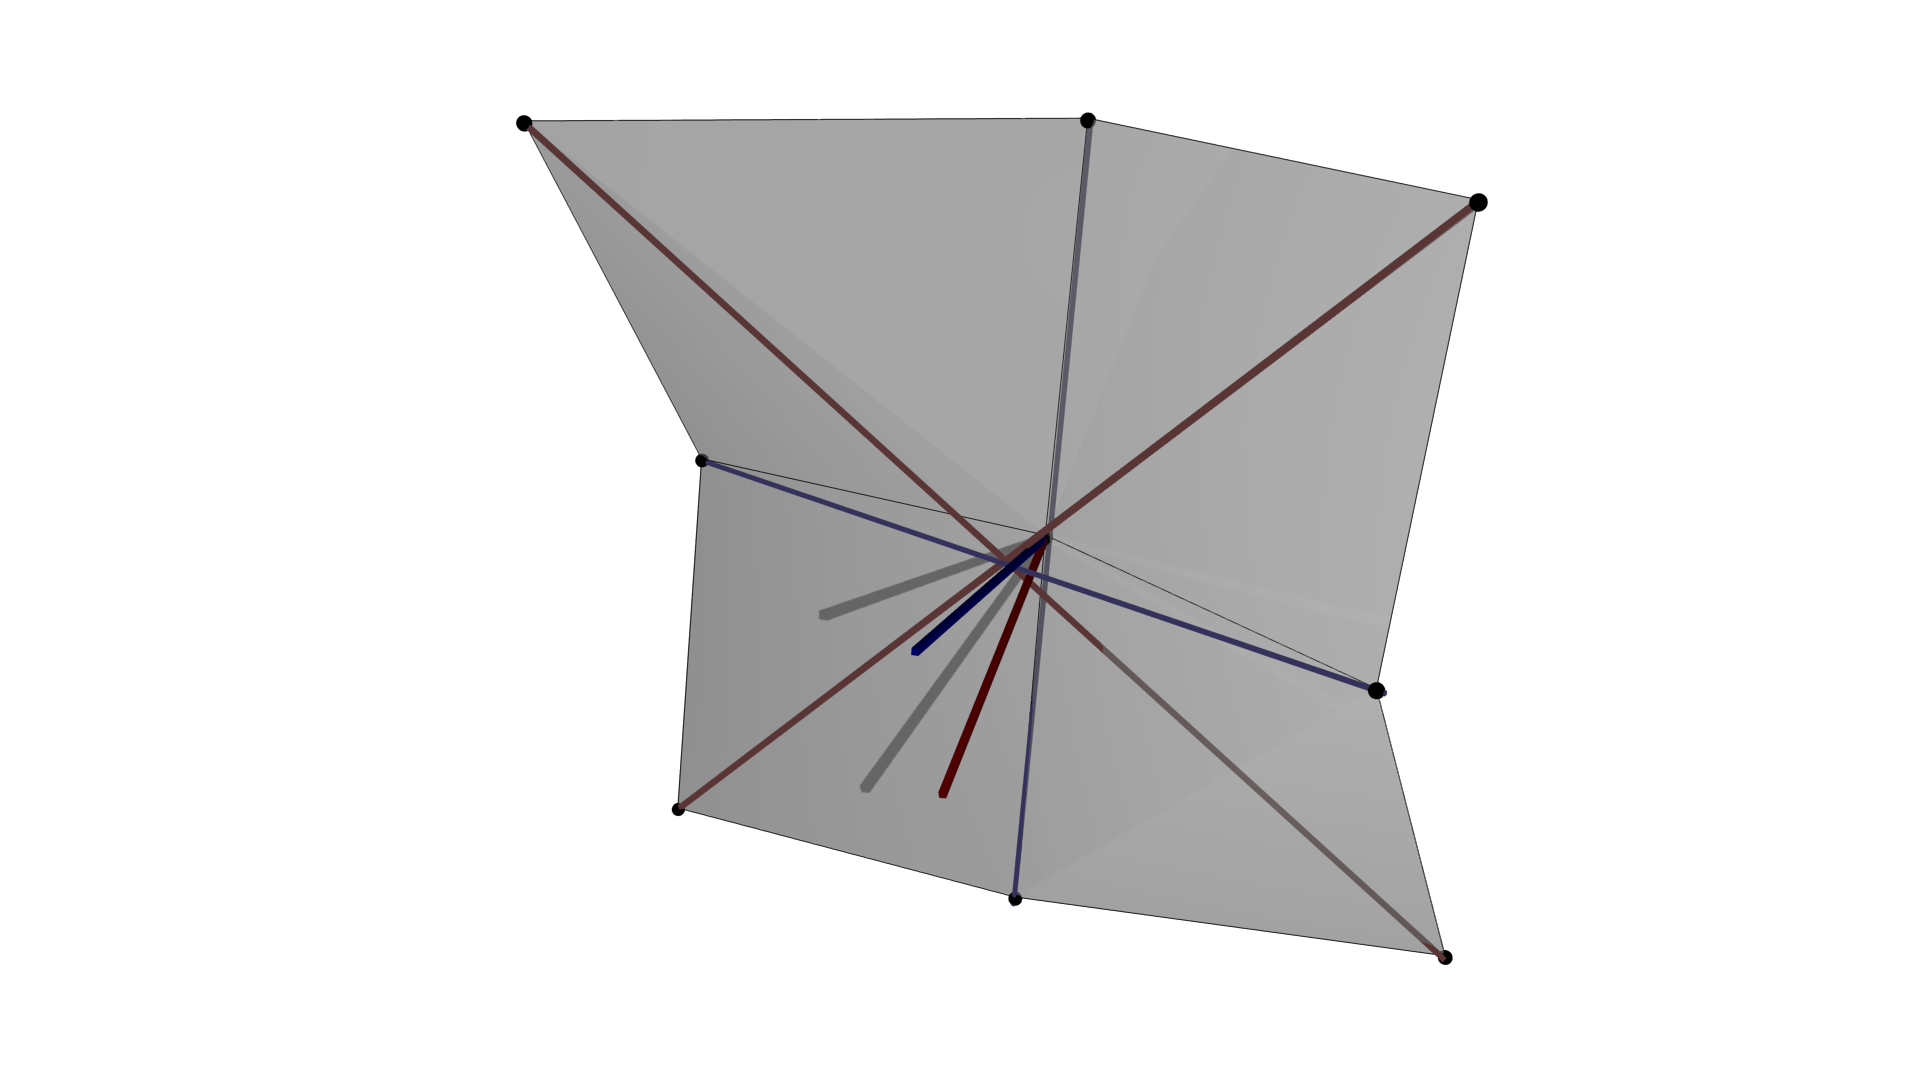
\includegraphics[width=0.9\textwidth]{chapter04/img/scetch_flexion.png}
    \end{subfigure}
    \begin{subfigure}[t]{0.49\linewidth}
        

\tikzset{every picture/.style={line width=0.75pt}} %set default line width to 0.75pt        

\begin{tikzpicture}[x=0.75pt,y=0.75pt,yscale=-1,xscale=1]
%uncomment if require: \path (0,237); %set diagram left start at 0, and has height of 237

%Shape: Rectangle [id:dp6565487036659107] 
\draw  [color={rgb, 255:red, 155; green, 155; blue, 155 }  ,draw opacity=1 ][dash pattern={on 4.5pt off 4.5pt}] (28.7,13.7) -- (206.3,13.7) -- (206.3,191.3) -- (28.7,191.3) -- cycle ;
%Straight Lines [id:da30195081571029425] 
\draw [color={rgb, 255:red, 74; green, 144; blue, 226 }  ,draw opacity=1 ] [dash pattern={on 4.5pt off 4.5pt}]  (28.7,102.5) -- (206.3,102.5) ;
%Straight Lines [id:da4586174781414081] 
\draw [color={rgb, 255:red, 74; green, 144; blue, 226 }  ,draw opacity=1 ] [dash pattern={on 4.5pt off 4.5pt}]  (117.5,13.7) -- (117.5,191.3) ;
%Straight Lines [id:da7294828306266232] 
\draw [color={rgb, 255:red, 245; green, 166; blue, 35 }  ,draw opacity=1 ] [dash pattern={on 4.5pt off 4.5pt}]  (28.7,13.7) -- (206.3,191.3) ;
%Straight Lines [id:da3243995266948473] 
\draw [color={rgb, 255:red, 245; green, 166; blue, 35 }  ,draw opacity=1 ] [dash pattern={on 4.5pt off 4.5pt}]  (28.7,191.3) -- (206.3,13.7) ;
%Shape: Circle [id:dp5266363779447065] 
\draw  [fill={rgb, 255:red, 245; green, 166; blue, 35 }  ,fill opacity=1 ] (25,13.7) .. controls (25,11.66) and (26.66,10) .. (28.7,10) .. controls (30.74,10) and (32.4,11.66) .. (32.4,13.7) .. controls (32.4,15.74) and (30.74,17.4) .. (28.7,17.4) .. controls (26.66,17.4) and (25,15.74) .. (25,13.7) -- cycle ;
%Shape: Ellipse [id:dp14497174740803043] 
\draw  [fill={rgb, 255:red, 74; green, 144; blue, 226 }  ,fill opacity=1 ] (25,102.5) .. controls (25,100.46) and (26.66,98.8) .. (28.7,98.8) .. controls (30.74,98.8) and (32.4,100.46) .. (32.4,102.5) .. controls (32.4,104.54) and (30.74,106.2) .. (28.7,106.2) .. controls (26.66,106.2) and (25,104.54) .. (25,102.5) -- cycle ;
%Shape: Ellipse [id:dp0427609892023727] 
\draw  [fill={rgb, 255:red, 245; green, 166; blue, 35 }  ,fill opacity=1 ] (25,191.3) .. controls (25,189.26) and (26.66,187.6) .. (28.7,187.6) .. controls (30.74,187.6) and (32.4,189.26) .. (32.4,191.3) .. controls (32.4,193.34) and (30.74,195) .. (28.7,195) .. controls (26.66,195) and (25,193.34) .. (25,191.3) -- cycle ;
%Shape: Ellipse [id:dp2872052196845898] 
\draw  [fill={rgb, 255:red, 74; green, 144; blue, 226 }  ,fill opacity=1 ] (113.8,13.7) .. controls (113.8,11.66) and (115.46,10) .. (117.5,10) .. controls (119.54,10) and (121.2,11.66) .. (121.2,13.7) .. controls (121.2,15.74) and (119.54,17.4) .. (117.5,17.4) .. controls (115.46,17.4) and (113.8,15.74) .. (113.8,13.7) -- cycle ;
%Shape: Circle [id:dp758793708555806] 
\draw  [fill={rgb, 255:red, 0; green, 0; blue, 0 }  ,fill opacity=1 ] (113.8,102.5) .. controls (113.8,100.46) and (115.46,98.8) .. (117.5,98.8) .. controls (119.54,98.8) and (121.2,100.46) .. (121.2,102.5) .. controls (121.2,104.54) and (119.54,106.2) .. (117.5,106.2) .. controls (115.46,106.2) and (113.8,104.54) .. (113.8,102.5) -- cycle ;
%Shape: Circle [id:dp477059334030714] 
\draw  [fill={rgb, 255:red, 74; green, 144; blue, 226 }  ,fill opacity=1 ] (113.8,191.3) .. controls (113.8,189.26) and (115.46,187.6) .. (117.5,187.6) .. controls (119.54,187.6) and (121.2,189.26) .. (121.2,191.3) .. controls (121.2,193.34) and (119.54,195) .. (117.5,195) .. controls (115.46,195) and (113.8,193.34) .. (113.8,191.3) -- cycle ;
%Shape: Ellipse [id:dp13207731000753575] 
\draw  [fill={rgb, 255:red, 245; green, 166; blue, 35 }  ,fill opacity=1 ] (202.6,13.7) .. controls (202.6,11.66) and (204.26,10) .. (206.3,10) .. controls (208.34,10) and (210,11.66) .. (210,13.7) .. controls (210,15.74) and (208.34,17.4) .. (206.3,17.4) .. controls (204.26,17.4) and (202.6,15.74) .. (202.6,13.7) -- cycle ;
%Shape: Circle [id:dp8288145253462365] 
\draw  [fill={rgb, 255:red, 74; green, 144; blue, 226 }  ,fill opacity=1 ] (202.6,102.5) .. controls (202.6,100.46) and (204.26,98.8) .. (206.3,98.8) .. controls (208.34,98.8) and (210,100.46) .. (210,102.5) .. controls (210,104.54) and (208.34,106.2) .. (206.3,106.2) .. controls (204.26,106.2) and (202.6,104.54) .. (202.6,102.5) -- cycle ;
%Shape: Circle [id:dp9160642610677009] 
\draw  [fill={rgb, 255:red, 245; green, 166; blue, 35 }  ,fill opacity=1 ] (202.6,191.3) .. controls (202.6,189.26) and (204.26,187.6) .. (206.3,187.6) .. controls (208.34,187.6) and (210,189.26) .. (210,191.3) .. controls (210,193.34) and (208.34,195) .. (206.3,195) .. controls (204.26,195) and (202.6,193.34) .. (202.6,191.3) -- cycle ;

% Text Node
\draw (106,110) node [anchor=north west][inner sep=0.75pt]   [align=left] {$\displaystyle \mathbf{P}_{i,j}$};
% Text Node
\draw (195,110) node [anchor=north west][inner sep=0.75pt]   [align=left] {$\displaystyle \mathbf{P}_{i+1,j}$};
% Text Node
\draw (16,110) node [anchor=north west][inner sep=0.75pt]   [align=left] {$\displaystyle \mathbf{P}_{i-1,j}$};
% Text Node
\draw (107,20) node [anchor=north west][inner sep=0.75pt]   [align=left] {$\displaystyle \mathbf{P}_{i,j-1}$};
% Text Node
\draw (196,20) node [anchor=north west][inner sep=0.75pt]   [align=left] {$\displaystyle \mathbf{P}_{i+1,j-1}$};
% Text Node
\draw (17,20) node [anchor=north west][inner sep=0.75pt]   [align=left] {$\displaystyle \mathbf{P}_{i-1,j-1}$};
% Text Node
\draw (106,200) node [anchor=north west][inner sep=0.75pt]   [align=left] {$\displaystyle \mathbf{P}_{i,j+1}$};
% Text Node
\draw (195,200) node [anchor=north west][inner sep=0.75pt]   [align=left] {$\displaystyle \mathbf{P}_{i+1,j+1}$};
% Text Node
\draw (16,200) node [anchor=north west][inner sep=0.75pt]   [align=left] {$\displaystyle \mathbf{P}_{i-1,j+1}$};


\end{tikzpicture}


    \end{subfigure}
    \caption[Schematic Representation of Flexion]{This figure demonstrates how flexed surfaces have different normals for diagonal and non-diagonal estimation. This difference is utilized as measure for flexion.}%
    \label{fig:flexion-image-scetched}
\end{figure}

The flexion $f$ is defined as
\begin{align}
    f &= \abs{n_1 \cdotp n_2}
\end{align}
Because $n_1$ and $n_2$ are of length $1$ the value of $f$ is in the range $[0, 1]$ and gets scaled accordingly.

The smaller the dot-product gets, the higher is the local flexion of the
surface. This local property of the geometry then results in visual
features detectable with classical feature detectors and descriptors like
\Gls{sift} or \Gls{surf}.

\subsubsection{Curvature}

\begin{figure}[H]
    \begin{subfigure}[t]{0.47\textwidth}
        \scalebox{0.9}{%
        \begin{tikzpicture}
\begin{axis}[xmin=-0.7,
             xmax=0.7,
             ymin=-0.1,
             ymax=1.1,
             samples=200,
             axis line style={draw=none},
             tick style={draw=none},
             xticklabels={\empty},
             yticklabels={\empty},
             grid=major,
             plot box ratio={2 1},
             axis equal]
    \draw[plotorange, line width=1.3pt] (axis cs:0,0.5) circle [radius=50];
    \addplot[plotblue, line width=1.5pt] {x*x};
    \coordinate (C) at (axis cs:{0.0,0.5});
    \coordinate (O) at (axis cs:{0.0,0.0});
    \coordinate (L) at (axis cs:{0.1,0.25});
    \node at (L) {$\mathbf{r}$};
    \node[label={90:{$\mathbf{C}$}},circle,fill,inner sep=1pt] at (C) {};
    \draw[thick,-](C)--(O);
\end{axis}
\end{tikzpicture}

        }
        \caption{The curvature of a line at a specific point is defined through its osculating circle.}
    \end{subfigure}
    \begin{subfigure}[t]{0.47\textwidth}
        \scalebox{0.9}{%
        \begin{tikzpicture}
\begin{axis}[xmin=-1.0,xmax=1.0,
             ymin=-1.0,ymax=1.0,
             zmin=-1.0,zmax=1.0,
             grid=major,
             axis line style={draw=none},
             tick style={draw=none},
             view={310}{35},
             xticklabels={\empty},
             yticklabels={\empty},
             zticklabels={\empty},
             plot box ratio={1 1 3},
             colormap/redyellow]
\newcommand\func[2]{#1^3 - #2^2}
\definecolor{darkorange}{HTML}{84644B}

    \addplot3[surf,
              shader=faceted interp,
              faceted color={darkorange},
              samples=15,
              domain=-1:1,
              y domain=-1:1] {\func{x}{y}};

    % plot curve for x direction
    \addplot3[samples=15,
              domain=-1:1,
              samples y=1,
              dotted,
              black,
              line width=1.1pt,
              smooth] (x, 0, \func{x}{0});
    % plot curve for y direction
    \addplot3[samples=15,
              domain=-1:1,
              y domain=-1:0.22,
              dotted,
              black,
              line width=1.1pt,
              smooth] (0, y, \func{0}{y});
\end{axis}
\end{tikzpicture}

        }
        \caption{The curvature of a surface at a given point depends on the direction of measurement. The principal curvatures are the maximum and minimum value of curvatures in all directions.}
    \end{subfigure}
\end{figure}

As a different analytical approach to producing feature images the calculation of the \gls{curvature} for each depth value.
The two common measures of curvature in differential geometry are \gls{gaussian-curvature} and \gls{mean-curvature}\cite{Kuhnel2008}.

If the function is known as a graph the \Gls{gaussian-curvature} can be estimated using the derivatives of the function.
For depth data each depth value is a sample of this function graph and numeric approximation of the derivatives allows the calculation of the curvature.
\begin{align}
    \mathfrak{K} &= \frac{f_{uu} f_{vv} - f_{uv}^2}{{(1 + f_u^2 + f_v^2)}^2}
\end{align}
With
\begin{align*}
    f_{x} &= \frac{y_1 - y_0}{\Delta x} \\
    f_{xx} &= \frac{y_1 + y_{-1} - 2 y_0}{{\Delta x}^2}
\end{align*}
as approximation for the derivatives.

Similarly, the \Gls{mean-curvature} can be calculated with a different formula.
\begin{align}
    \mathfrak{H} &= \frac{{(1 + f_{v}^2)} f_{uu} - 2 f_u f_v f_{uv} + {(1 + f_u^2)} f_{vv}}{2 \sqrt{1 + f_u^2 + f_v^2}^3}
\end{align}
Both measures of curvature are $\mathfrak{K},\mathfrak{H} \in {\rm I\!R}$.
To convert them into a meaningful grayscale image they need to be clamped to arbitrary bounds, that can be choosen based on visual distinctiveness or other heuristics.
After clamping the values are scaled and quantized accordingly.

\subsubsection{Multi-Directional Bearing Angle}

The \gls{max-curve-image} tries generalize the \gls{bearing-angle} to be rotation invariant as it takes the \gls{bearing-angle} in each direction into account.
Additionally to the left-sided \gls{bearing-angle} the right-sided angle is calculated as well and finally added.

\begin{figure}
    

\tikzset{every picture/.style={line width=0.75pt}} %set default line width to 0.75pt        

\begin{tikzpicture}[x=0.75pt,y=0.75pt,yscale=-1,xscale=1]
%uncomment if require: \path (0,252); %set diagram left start at 0, and has height of 252

%Straight Lines [id:da05017383740499093] 
\draw    (46.83,26.67) -- (149.83,213.67) ;
%Straight Lines [id:da6895513561877372] 
\draw    (155.83,32.67) -- (149.83,213.67) ;
%Curve Lines [id:da10253757735662583] 
\draw [color={rgb, 255:red, 0; green, 0; blue, 0 }  ,draw opacity=1 ]   (116,153) .. controls (128.83,126.67) and (169.83,125.67) .. (181.83,145.67) ;
%Straight Lines [id:da3851492122035306] 
\draw    (46.83,26.67) -- (155.83,32.67) ;
%Shape: Circle [id:dp08101382020617043] 
\draw  [fill={rgb, 255:red, 0; green, 0; blue, 0 }  ,fill opacity=1 ] (151.88,32.67) .. controls (151.88,30.49) and (153.65,28.72) .. (155.83,28.72) .. controls (158.01,28.72) and (159.78,30.49) .. (159.78,32.67) .. controls (159.78,34.85) and (158.01,36.62) .. (155.83,36.62) .. controls (153.65,36.62) and (151.88,34.85) .. (151.88,32.67) -- cycle ;
%Shape: Circle [id:dp7397482298206297] 
\draw  [fill={rgb, 255:red, 0; green, 0; blue, 0 }  ,fill opacity=1 ] (42.88,26.67) .. controls (42.88,24.49) and (44.65,22.72) .. (46.83,22.72) .. controls (49.01,22.72) and (50.78,24.49) .. (50.78,26.67) .. controls (50.78,28.85) and (49.01,30.62) .. (46.83,30.62) .. controls (44.65,30.62) and (42.88,28.85) .. (42.88,26.67) -- cycle ;
%Shape: Circle [id:dp7936487176657823] 
\draw  [fill={rgb, 255:red, 0; green, 0; blue, 0 }  ,fill opacity=1 ] (241.88,7.67) .. controls (241.88,5.49) and (243.65,3.72) .. (245.83,3.72) .. controls (248.01,3.72) and (249.78,5.49) .. (249.78,7.67) .. controls (249.78,9.85) and (248.01,11.62) .. (245.83,11.62) .. controls (243.65,11.62) and (241.88,9.85) .. (241.88,7.67) -- cycle ;
%Straight Lines [id:da7225304487809803] 
\draw    (245.83,7.67) -- (149.83,213.67) ;
%Straight Lines [id:da15289701870660388] 
\draw    (155.83,32.67) -- (245.83,7.67) ;
%Shape: Arc [id:dp845909277560968] 
\draw  [draw opacity=0] (154.29,72.43) .. controls (153.16,72.54) and (152.02,72.6) .. (150.87,72.6) .. controls (131.56,72.6) and (115.9,56.94) .. (115.9,37.63) .. controls (115.9,35.08) and (116.17,32.59) .. (116.69,30.19) -- (150.87,37.63) -- cycle ; \draw  [color={rgb, 255:red, 208; green, 2; blue, 27 }  ,draw opacity=1 ] (154.29,72.43) .. controls (153.16,72.54) and (152.02,72.6) .. (150.87,72.6) .. controls (131.56,72.6) and (115.9,56.94) .. (115.9,37.63) .. controls (115.9,35.08) and (116.17,32.59) .. (116.69,30.19) ;
%Shape: Arc [id:dp15343497156889918] 
\draw  [draw opacity=0] (193.67,22.29) .. controls (195.16,26.33) and (195.97,30.7) .. (195.97,35.25) .. controls (195.97,55.99) and (179.15,72.8) .. (158.42,72.8) .. controls (157.06,72.8) and (155.72,72.73) .. (154.4,72.59) -- (158.42,35.25) -- cycle ; \draw  [color={rgb, 255:red, 245; green, 166; blue, 35 }  ,draw opacity=1 ] (193.67,22.29) .. controls (195.16,26.33) and (195.97,30.7) .. (195.97,35.25) .. controls (195.97,55.99) and (179.15,72.8) .. (158.42,72.8) .. controls (157.06,72.8) and (155.72,72.73) .. (154.4,72.59) ;

% Text Node
\draw (137,154) node  [color={rgb, 255:red, 0; green, 0; blue, 0 }  ,opacity=1 ] [align=left] {$\displaystyle \Delta $$\displaystyle \varphi $};
% Text Node
\draw (138,48) node  [color={rgb, 255:red, 208; green, 2; blue, 27 }  ,opacity=1 ] [align=left] {$\displaystyle \beta $};
% Text Node
\draw (169,100) node   [align=left] {$\displaystyle d_{i,j}$};
% Text Node
\draw (65,100) node   [align=left] {$\displaystyle d_{i-1,j}$};
% Text Node
\draw (154,12) node   [align=left] {$\displaystyle \mathbf{P}_{i,j}$};
% Text Node
\draw (150,226) node   [align=left] {$\displaystyle \mathbf{C}$};
% Text Node
\draw (232,99) node   [align=left] {$\displaystyle d_{i+1,j}$};
% Text Node
\draw (172,48) node   [align=left] {$\displaystyle \textcolor[rgb]{0.96,0.65,0.14}{\gamma }$};
% Text Node
\draw (165,154) node  [color={rgb, 255:red, 0; green, 0; blue, 0 }  ,opacity=1 ] [align=left] {$\displaystyle \Delta $$\displaystyle \theta $};
% Text Node
\draw (273,12) node   [align=left] {$\displaystyle \mathbf{P}_{i+1,j}$};
% Text Node
\draw (24,12) node   [align=left] {$\displaystyle \mathbf{P}_{i-1,j}$};


\end{tikzpicture}


    \caption[Schematic Representation of the Max-Curve]{The Max-Curve composes two \Glspl{bearing-angle} in vertical, horizontal, diagonal and antidiagonal direction. The maximum angle is then selected as pixel value.}
\end{figure}

This makes the measure more robust to rotation, but does not produce good features.
\begin{align}
    B &= \max{\{B_{diagonal}, B_{antidiagonal}, B_{horizontal}, B_{vertical}\}}
\end{align}

\subsubsection{Viability of Conversions}

\begin{itemize}
    \item effect of noisy input
    \item soundness and mathematical foundation
    \item computational complexity
    \item Discussion of characteristic for Bearing Flexion.
\end{itemize}

\subsubsection{Implementation Notes}

Formulas pictures and short computational evaluation.
Each implementation is independent of the camera model.
Describe the concepts required for implementation.
Both serial and parallel execution.
Parallel execution is done row-wise over all cores using CppTaskflow based Task Scheduling.
No explicit use SIMD, because OpenCV\cite{opencv_library} is used for data storing proper memory alignment is already ensured.
Specialized optimiziation should allow the use of SIMD with OpenCV's Hardware Abstraction Layer.

Focus on correctness and generality.
Provided implementation should rather serve as reference implementation that can be used to validate optimized implementations.

\begin{lstlisting}
template <template <typename> typename Intrinsic,
          typename Real>
inline constexpr bool is_intrinsic_v =
  std::is_floating_point_v<Real>
  &&
  std::is_same_v<typename Intrinsic<Real>::real_type, Real>
  &&
  std::is_invocable_r_v<
    int,
    decltype(&Intrinsic<Real>::w),
    Intrinsic<Real>
  >
  &&
  std::is_invocable_r_v<
    int,
    decltype(&Intrinsic<Real>::h),
    Intrinsic<Real>
  >
  &&
  std::is_invocable_r_v<
    math::sphere_coord<Real>,
    decltype(&Intrinsic<Real>::template pixel_to_sphere<int>),
    Intrinsic<Real>,
    math::pixel_coord<int>
  >
  &&
  std::is_invocable_r_v<
    math::sphere_coord<Real>,
    decltype(&Intrinsic<Real>::template pixel_to_sphere<Real>),
    Intrinsic<Real>,
    math::pixel_coord<Real>
  >
  &&
  std::is_invocable_r_v<
    math::pixel_coord<Real>,
    decltype(&Intrinsic<Real>::template camera_to_pixel<Real>),
    Intrinsic<Real>,
    math::camera_coord<Real>
  >
  &&
  std::is_invocable_r_v<
    math::pixel_coord<int>,
    decltype(&Intrinsic<Real>::template camera_to_pixel<int>),
    Intrinsic<Real>,
    math::camera_coord<Real>
  >;
\end{lstlisting}


\subsection{Feature Detection and Description}\label{sec:feature_algorithms}

After preprocessing and image conversion, the final processing step of the range data is the feature detection and description.
This thesis analyzes \acrshort{sift}\cite{lowe_ijcv04}, \acrshort{surf}\cite{bay_eccv06}, \acrshort{orb}\cite{rublee_iccv11} and \acrshort{akaze}\cite{alcantarilla_bmva13}.
Although each keypoint detector and descriptor is designed with gray-scale images in mind, they are optimized for classical camera images that provide more texture than the converted feature images.
Key to all algorithms is the search for salient regions in the image that can be consistently detected from different viewpoints and changing environmental conditions.
The detector performance is critical to apply classical image registration approaches to the converted feature images.
The following sections introduce the algorithms briefly and mentions key aspects of their functionality.
Details and foundational concepts are out of scope and the original publications are highly recommended for further comprehension.

\subsubsection{\acrshort{sift} (\acrlong{sift})}

Introduced by Lowe\cite{lowe_iccv99,lowe_ijcv04}, \acrshort{sift} is an established feature detection algorithm.
The design goal of the algorithm is to detect keypoints that are invariant with respect to scale and rotation.
Robustness against noise, change in illumination and affine transformations is additionally considered.
\acrshort{sift}'s design influenced the design decisions of the other presented algorithms heavily.

The input image is processed in a hierarchical pyramid of down-scaled versions of the image, called octaves.
On each octave a Gaussian filter is applied consecutively with increased standard deviation on each run.
The difference between two consecutive blurred images is computed, the so called \acrlong{DoG} (\acrshort{DoG}) forming an approximation of the Laplacian of the image.
Lindeberg's\cite{lindeberg_ijcv98} work on scale space and automatic scale selection gives a theoretical introduction why this process gives a good way to select the scale of features.
The underlying principle exploits that fine structures dissolve at bigger scales.
This process is related to the diffusion equation that is strongly tied to the Laplacian of the image.
Keypoint candidates are local extrema in these \acrshort{DoG}s.
Each candidate is filtered by a contrast threshold, its accurate position is determined using a local spline interpolation and its scale is assigned based on the octave and blurring factor.
Edge-like responses are filtered out based on an estimate of the ratio between the principal curvatures.
Highly skewed curvatures indicate an edge.

Every keypoint candidate gets one or more orientations assigned.
These are computed by storing the gradients of a local neighbourhood to the keypoints in the octave matching the keypoints scale in an orientation histogram.
Each peak in this histogram reflects a dominant direction of gradients in the local neighbourhood and the corresponding angle is used as the orientation of the keypoint.
According to Lowe\cite{lowe_ijcv04}, about 15\% of keypoints have multiple peaks and get multiple orientations assigned.
The orientation is used to rotate the local neighbourhood of the keypoint to compute the descriptor consistently.

The image gradients direction and magnitude are computed for each pixel in a local environment, first weighted by a Gaussian to magnify the influence of close pixels and then binned into orientation histograms.
Each histogram reflects a fraction of the sampling grid.
A 16$\times$16 grid around the keypoint that is stored to 4$\times$4 histograms with 8 bins for the orientations results in a vector of 128 elements in the descriptor.
These dimensions can be adjusted, but the 128 element descriptor is most common.
Finally, the histograms are normalized to increase robustness against illumination changes.
The Euclidean distance of the descriptor vectors is the most common similarity measure.
Arandjelović and Zisserman\cite{arandjelovic_2012} introduced RootSIFT using the Hellinger distance\cite{hellinger_1909} as better measure for similarity of histograms.

\subsubsection{\acrshort{surf} (\acrlong{surf})}

Bay et al. introduced \acrshort{surf}\cite{bay_eccv06} to achieve similar detector and descriptor performance as \acrshort{sift} but at a lower computational cost.
\acrshort{surf} utilizes integral images\cite{viola_cvpr01}.
Each pixel's value is the sum of all pixels in the rectangle formed by the origin and the pixel itself.
This representation reduces computational complexity.

The underlying principal of scale space and extrema detection derives from the same principles as for \acrshort{sift} but undergoes simplification.
The Gaussian convolution is approximated with a box filter that approximate a second order Gaussian derivative and is related to the Hessian matrix.
Instead of building a pyramid of images at different scales, the filter itself is scaled up successively.
Maxima undergo a non-maximum suppression at different scales.
The maximum of the Hessian determinant for the detected pixel is interpolated in image scale and space.
The determinants value is the keypoint's response.

Orientation assignment of \acrshort{surf} can be skipped for scenarios that do not involve camera rotation.
The rotation is derived from the Haar wavelets\cite{haar_1911} response in $x$ and $y$ direction in the local neighbourhood.
The descriptor itself is constructed from a 4$\times$4 grid structure of sample points around the detected keypoint.
Again, the Haar wavelets response in $x$ and $y$ direction are used to derive the elements of the descriptor.

\subsubsection{\acrshort{orb} (\acrlong{orb})}

\acrshort{orb}\cite{rublee_iccv11} combines the \acrshort{fast}\cite{rosten_eccv06} (\acrlong{fast}) feature detector and \acrshort{brief}\cite{calonder_eccv10} (\acrlong{brief}) descriptor with additional improvements to both algorithms.
The design goal is to achieve similar matching performance to \acrshort{sift} and \acrshort{surf} but to be computationally cheaper to make usage in embedded devices feasible.

The \acrshort{fast} detector evaluates a each pixel by testing the brightness of 16~pixels on a circle around the corner.
If there are enough consecutive pixels brighter or darker than the center with a certain threshold, the pixel is accepted as corner.
This approach results in a decision tree.
The optimal traversal of this tree is learned by observing real world execution of the algorithm on predefined traversal.
\acrshort{orb} detects keypoints with \acrshort{fast}, filters edge results with the Harris corner detector\cite{harris_1988} and assigns scale using image pyramids.
The orientation of the keypoint is computed with the \emph{intensity centroid}\cite{rosin_cviu99}.

Each keypoint's descriptor uses a rotated version of \acrshort{brief}.
\acrshort{brief} is a binary descriptor built from a set of binary intensity tests of consecutive pixels around the keypoint.
The more recent publications, like \acrshort{brief}, \acrshort{orb} and \acrshort{mldb}, employ binary descriptors for their fast matching speed.
The distance of binary descriptors can be computed with the Hamming distance that reduces to \emph{XOR} instructions on machine level.
Ziegler et al.\cite{ziegler_anips2012} provide a theoretical analysis of \acrshort{brief} and its siblings and show, that those are hashing schemes of Kendall's $\tau$ metric\cite{kendall_1938}.

\subsubsection{\acrshort{akaze}}

\acrshort{kaze}'s\cite{alcantarilla_eccv12} (\acrlong{kaze}) and \acrshort{akaze}'s\cite{alcantarilla_bmva13} (\acrlong{akaze}) approaches are similar to \acrshort{sift}'s.
Again, the diffusion of the brightness is the starting point for scale space analysis.
\acrshort{kaze} applies non-linear diffusion filtering with a special computational scheme, that makes it feasible to solve the diffusion in real time.
The difference to the Gaussian blurring is the preservation of edges.
The Gaussian blurs the whole image, reducing the signal crispness at higher scales.
Contrary, the non-linear diffusion preserves edges over higher scales.
After non-maximum suppression, the determinant of the Hessian is computed and the interpolation of the maximum on different scales yields the position of the keypoint.
The orientation of the keypoint is, similar to \acrshort{sift}, the dominant direction of the derivatives in the local neighbourhood of the keypoint.

The descriptor is \acrshort{mldb} (\acrlong{mldb}), which is based on \acrshort{ldb}\cite{yang_ismar12} (\acrlong{ldb}).
It works very similar to \acrshort{brief}.
But instead of comparing intensities of sampled pixel, it compares the average intensities of sampled areas around the keypoint.
The orientation of the keypoint is taken into account when sampling the areas.

\newpage

\section{Experiments}\label{sec:experiments}

The experiments evaluate the performance the \gls{bearing-angle} and \gls{flexion-image} for a variety of sensors, datasets and processing setups.
They demonstrate both success and failure under certain circumstances.
Both qualitative and quantitative are considered in the evaluation.
Section~\ref{sec:results} discusses these results.

\subsection{Metrics}

To determine the performance of the feature-based approach, the matching of keypoints is framed in terms of a binary classifier.
For a keypoint correspondence between two images, the classification task is to determine if those keypoints correspond to the same point in the real world or not.
The correspondence is computed based on the relative pose of consecutive images and only two consecutive images are analyzed.
The following subsections describe each component of this evaluation pipeline in more detail.

\subsubsection{Ground Truth Poses}

The dataset \emph{Mine} provides ground truth poses from a prior \gls{sfm} reconstruction.
Due to the global optimization of the \gls{sfm} algorithm, these poses do not match with the depth values of the depth images.
The other datasets do not contain a precomputed pose.
Therefore, each pose is computed and refined with an ICP algorithm, namely OpenCV's \texttt{FASTICPOdometry}\cite{opencv_library} that is based on the KinectFusion\cite{newcombe_ismar2011} work.
This relative pose serves as foundation of the evaluation and is assumed to be correct within small tolerance.
The accuracy assumption of the \texttt{FASTICPOdometry} poses is tested by manual inspection of the backprojection of obviously related keypoints and the results showed no systematic erroneous poses.

\subsubsection{Backprojection and Distance Threshold}

In two consecutive images, all keypoints are extracted with the chosen algorithm and settings.
Each keypoint of the first image $I_1$ is projected to the unit sphere, e.g. with Equation~\ref{eq:pinhole_backward}, multiplied with the range value of the corresponding pixel.
The resulting camera coordinate is transformed to the second camera coordinate system (Equation~\ref{eq:homogeneous_matrix}).
Projecting the keypoint into the second camera with the matching forward projection (e.g. Equation~\ref{eq:pinhole_forward}) finalizes the procedure, demonstrated in Figure~\ref{fig:keypoint_projection}.
This results in two sets of keypoints in the second image $I_2$, the keypoints detected in this frame and the keypoints detected in the previous frame, seen from this frame's pose.
Assuming a correct relative pose, the corresponding keypoints have a small pixel distance between each other.
\emph{Small} is a relative value and the chosen threshold in the experiments is 2\,px.
This approach can only result in a proper analysis for a sparse distribution of keypoints that actually correspond to image structure and requires small changes in pose.
When the pose difference is big, it can happen that keypoints get projected to the same position as some other valid keypoint without referencing the same world point.
Too many points create ambiguity with respect to the backprojection tolerance.
\begin{figure}[b!]
    

\tikzset{every picture/.style={line width=0.75pt}} %set default line width to 0.75pt        

\begin{tikzpicture}[x=0.75pt,y=0.75pt,yscale=-1,xscale=1]
%uncomment if require: \path (0,229); %set diagram left start at 0, and has height of 229

%Shape: Rectangle [id:dp6786998235335104] 
\draw   (21.88,21.67) -- (253.33,21.67) -- (253.33,189.54) -- (21.88,189.54) -- cycle ;
%Shape: Polygon [id:ds4691410097865978] 
\draw  [fill={rgb, 255:red, 0; green, 0; blue, 0 }  ,fill opacity=1 ] (127.01,83.56) -- (164.31,128.49) -- (111.75,109) -- (64.27,123.41) -- (60.88,86.1) -- cycle ;
%Shape: Circle [id:dp07615520367165762] 
\draw  [draw opacity=0][fill={rgb, 255:red, 74; green, 144; blue, 226 }  ,fill opacity=1 ] (160.08,128.49) .. controls (160.08,126.15) and (161.97,124.26) .. (164.31,124.26) .. controls (166.66,124.26) and (168.55,126.15) .. (168.55,128.49) .. controls (168.55,130.84) and (166.66,132.73) .. (164.31,132.73) .. controls (161.97,132.73) and (160.08,130.84) .. (160.08,128.49) -- cycle ;
%Shape: Ellipse [id:dp6448504150595761] 
\draw  [draw opacity=0][fill={rgb, 255:red, 74; green, 144; blue, 226 }  ,fill opacity=1 ] (122.77,83.56) .. controls (122.77,81.22) and (124.67,79.32) .. (127.01,79.32) .. controls (129.35,79.32) and (131.25,81.22) .. (131.25,83.56) .. controls (131.25,85.9) and (129.35,87.8) .. (127.01,87.8) .. controls (124.67,87.8) and (122.77,85.9) .. (122.77,83.56) -- cycle ;
%Shape: Ellipse [id:dp7051810352399743] 
\draw  [draw opacity=0][fill={rgb, 255:red, 74; green, 144; blue, 226 }  ,fill opacity=1 ] (107.51,109) .. controls (107.51,106.65) and (109.41,104.76) .. (111.75,104.76) .. controls (114.09,104.76) and (115.99,106.65) .. (115.99,109) .. controls (115.99,111.34) and (114.09,113.23) .. (111.75,113.23) .. controls (109.41,113.23) and (107.51,111.34) .. (107.51,109) -- cycle ;
%Shape: Ellipse [id:dp9159085548976601] 
\draw  [draw opacity=0][fill={rgb, 255:red, 74; green, 144; blue, 226 }  ,fill opacity=1 ] (60.04,123.41) .. controls (60.04,121.07) and (61.93,119.17) .. (64.27,119.17) .. controls (66.62,119.17) and (68.51,121.07) .. (68.51,123.41) .. controls (68.51,125.75) and (66.62,127.65) .. (64.27,127.65) .. controls (61.93,127.65) and (60.04,125.75) .. (60.04,123.41) -- cycle ;
%Shape: Ellipse [id:dp49160949647303864] 
\draw  [draw opacity=0][fill={rgb, 255:red, 74; green, 144; blue, 226 }  ,fill opacity=1 ] (56.64,86.1) .. controls (56.64,83.76) and (58.54,81.87) .. (60.88,81.87) .. controls (63.22,81.87) and (65.12,83.76) .. (65.12,86.1) .. controls (65.12,88.45) and (63.22,90.34) .. (60.88,90.34) .. controls (58.54,90.34) and (56.64,88.45) .. (56.64,86.1) -- cycle ;
%Shape: Polygon [id:ds13360398877823854] 
\draw  [fill={rgb, 255:red, 0; green, 0; blue, 0 }  ,fill opacity=1 ] (201.67,91.58) -- (232.66,121.16) -- (210.12,157.78) -- (191.81,131.01) -- cycle ;
%Shape: Ellipse [id:dp8706054475141728] 
\draw  [draw opacity=0][fill={rgb, 255:red, 74; green, 144; blue, 226 }  ,fill opacity=1 ] (205.89,157.78) .. controls (205.89,155.43) and (207.78,153.54) .. (210.12,153.54) .. controls (212.47,153.54) and (214.36,155.43) .. (214.36,157.78) .. controls (214.36,160.12) and (212.47,162.01) .. (210.12,162.01) .. controls (207.78,162.01) and (205.89,160.12) .. (205.89,157.78) -- cycle ;
%Shape: Circle [id:dp6356920604931994] 
\draw  [draw opacity=0][fill={rgb, 255:red, 74; green, 144; blue, 226 }  ,fill opacity=1 ] (228.42,121.16) .. controls (228.42,118.81) and (230.32,116.92) .. (232.66,116.92) .. controls (235,116.92) and (236.9,118.81) .. (236.9,121.16) .. controls (236.9,123.5) and (235,125.39) .. (232.66,125.39) .. controls (230.32,125.39) and (228.42,123.5) .. (228.42,121.16) -- cycle ;
%Shape: Ellipse [id:dp943196171409342] 
\draw  [draw opacity=0][fill={rgb, 255:red, 74; green, 144; blue, 226 }  ,fill opacity=1 ] (197.43,91.58) .. controls (197.43,89.24) and (199.33,87.34) .. (201.67,87.34) .. controls (204.01,87.34) and (205.91,89.24) .. (205.91,91.58) .. controls (205.91,93.92) and (204.01,95.82) .. (201.67,95.82) .. controls (199.33,95.82) and (197.43,93.92) .. (197.43,91.58) -- cycle ;
%Shape: Ellipse [id:dp15135575228311182] 
\draw  [draw opacity=0][fill={rgb, 255:red, 74; green, 144; blue, 226 }  ,fill opacity=1 ] (187.58,131.01) .. controls (187.58,128.67) and (189.47,126.78) .. (191.81,126.78) .. controls (194.16,126.78) and (196.05,128.67) .. (196.05,131.01) .. controls (196.05,133.36) and (194.16,135.25) .. (191.81,135.25) .. controls (189.47,135.25) and (187.58,133.36) .. (187.58,131.01) -- cycle ;
%Shape: Circle [id:dp9787468728029534] 
\draw  [draw opacity=0][fill={rgb, 255:red, 74; green, 144; blue, 226 }  ,fill opacity=1 ] (125.6,170.45) .. controls (125.6,168.11) and (127.5,166.21) .. (129.84,166.21) .. controls (132.18,166.21) and (134.08,168.11) .. (134.08,170.45) .. controls (134.08,172.79) and (132.18,174.69) .. (129.84,174.69) .. controls (127.5,174.69) and (125.6,172.79) .. (125.6,170.45) -- cycle ;
%Shape: Circle [id:dp6723223909711141] 
\draw  [draw opacity=0][fill={rgb, 255:red, 74; green, 144; blue, 226 }  ,fill opacity=1 ] (65.04,162) .. controls (65.04,159.66) and (66.94,157.76) .. (69.28,157.76) .. controls (71.62,157.76) and (73.52,159.66) .. (73.52,162) .. controls (73.52,164.34) and (71.62,166.24) .. (69.28,166.24) .. controls (66.94,166.24) and (65.04,164.34) .. (65.04,162) -- cycle ;
%Shape: Ellipse [id:dp7974562368161737] 
\draw  [draw opacity=0][fill={rgb, 255:red, 74; green, 144; blue, 226 }  ,fill opacity=1 ] (170.66,59.62) .. controls (170.66,57.28) and (172.56,55.38) .. (174.9,55.38) .. controls (177.24,55.38) and (179.14,57.28) .. (179.14,59.62) .. controls (179.14,61.96) and (177.24,63.86) .. (174.9,63.86) .. controls (172.56,63.86) and (170.66,61.96) .. (170.66,59.62) -- cycle ;
%Shape: Ellipse [id:dp723151821080846] 
\draw  [draw opacity=0][fill={rgb, 255:red, 74; green, 144; blue, 226 }  ,fill opacity=1 ] (70.66,52.58) .. controls (70.66,50.23) and (72.56,48.34) .. (74.9,48.34) .. controls (77.24,48.34) and (79.14,50.23) .. (79.14,52.58) .. controls (79.14,54.92) and (77.24,56.81) .. (74.9,56.81) .. controls (72.56,56.81) and (70.66,54.92) .. (70.66,52.58) -- cycle ;
%Shape: Polygon [id:ds8593635117147446] 
\draw  [fill={rgb, 255:red, 0; green, 0; blue, 0 }  ,fill opacity=1 ] (360.05,83.39) -- (397.35,128.33) -- (344.79,108.83) -- (297.31,123.24) -- (293.92,85.94) -- cycle ;
%Shape: Ellipse [id:dp989610403946918] 
\draw  [color={rgb, 255:red, 245; green, 166; blue, 35 }  ,draw opacity=1 ][fill={rgb, 255:red, 74; green, 144; blue, 226 }  ,fill opacity=1 ][line width=1.5]  (393.11,128.33) .. controls (393.11,125.99) and (395.01,124.09) .. (397.35,124.09) .. controls (399.69,124.09) and (401.59,125.99) .. (401.59,128.33) .. controls (401.59,130.67) and (399.69,132.57) .. (397.35,132.57) .. controls (395.01,132.57) and (393.11,130.67) .. (393.11,128.33) -- cycle ;
%Shape: Ellipse [id:dp5019836404546896] 
\draw  [color={rgb, 255:red, 245; green, 166; blue, 35 }  ,draw opacity=1 ][fill={rgb, 255:red, 74; green, 144; blue, 226 }  ,fill opacity=1 ][line width=1.5]  (355.81,83.39) .. controls (355.81,81.05) and (357.71,79.15) .. (360.05,79.15) .. controls (362.39,79.15) and (364.29,81.05) .. (364.29,83.39) .. controls (364.29,85.74) and (362.39,87.63) .. (360.05,87.63) .. controls (357.71,87.63) and (355.81,85.74) .. (355.81,83.39) -- cycle ;
%Shape: Ellipse [id:dp7578792049912161] 
\draw  [color={rgb, 255:red, 245; green, 166; blue, 35 }  ,draw opacity=1 ][fill={rgb, 255:red, 74; green, 144; blue, 226 }  ,fill opacity=1 ][line width=1.5]  (340.55,108.83) .. controls (340.55,106.49) and (342.45,104.59) .. (344.79,104.59) .. controls (347.13,104.59) and (349.03,106.49) .. (349.03,108.83) .. controls (349.03,111.17) and (347.13,113.07) .. (344.79,113.07) .. controls (342.45,113.07) and (340.55,111.17) .. (340.55,108.83) -- cycle ;
%Shape: Ellipse [id:dp2443027365226711] 
\draw  [color={rgb, 255:red, 245; green, 166; blue, 35 }  ,draw opacity=1 ][fill={rgb, 255:red, 74; green, 144; blue, 226 }  ,fill opacity=1 ][line width=1.5]  (293.07,123.24) .. controls (293.07,120.9) and (294.97,119) .. (297.31,119) .. controls (299.65,119) and (301.55,120.9) .. (301.55,123.24) .. controls (301.55,125.58) and (299.65,127.48) .. (297.31,127.48) .. controls (294.97,127.48) and (293.07,125.58) .. (293.07,123.24) -- cycle ;
%Shape: Ellipse [id:dp9130120394048863] 
\draw  [color={rgb, 255:red, 245; green, 166; blue, 35 }  ,draw opacity=1 ][fill={rgb, 255:red, 74; green, 144; blue, 226 }  ,fill opacity=1 ][line width=1.5]  (289.68,85.94) .. controls (289.68,83.6) and (291.58,81.7) .. (293.92,81.7) .. controls (296.26,81.7) and (298.16,83.6) .. (298.16,85.94) .. controls (298.16,88.28) and (296.26,90.18) .. (293.92,90.18) .. controls (291.58,90.18) and (289.68,88.28) .. (289.68,85.94) -- cycle ;
%Shape: Polygon [id:ds05866278290858706] 
\draw  [fill={rgb, 255:red, 0; green, 0; blue, 0 }  ,fill opacity=1 ] (434.71,91.41) -- (465.7,120.99) -- (443.16,157.61) -- (424.85,130.85) -- cycle ;
%Shape: Ellipse [id:dp03726801994871687] 
\draw  [color={rgb, 255:red, 245; green, 166; blue, 35 }  ,draw opacity=1 ][fill={rgb, 255:red, 74; green, 144; blue, 226 }  ,fill opacity=1 ][line width=1.5]  (438.92,157.61) .. controls (438.92,155.27) and (440.82,153.37) .. (443.16,153.37) .. controls (445.5,153.37) and (447.4,155.27) .. (447.4,157.61) .. controls (447.4,159.95) and (445.5,161.85) .. (443.16,161.85) .. controls (440.82,161.85) and (438.92,159.95) .. (438.92,157.61) -- cycle ;
%Shape: Ellipse [id:dp8191161671737491] 
\draw  [color={rgb, 255:red, 245; green, 166; blue, 35 }  ,draw opacity=1 ][fill={rgb, 255:red, 74; green, 144; blue, 226 }  ,fill opacity=1 ][line width=1.5]  (461.46,120.99) .. controls (461.46,118.65) and (463.35,116.75) .. (465.7,116.75) .. controls (468.04,116.75) and (469.93,118.65) .. (469.93,120.99) .. controls (469.93,123.33) and (468.04,125.23) .. (465.7,125.23) .. controls (463.35,125.23) and (461.46,123.33) .. (461.46,120.99) -- cycle ;
%Shape: Ellipse [id:dp09089598583753888] 
\draw  [color={rgb, 255:red, 245; green, 166; blue, 35 }  ,draw opacity=1 ][fill={rgb, 255:red, 74; green, 144; blue, 226 }  ,fill opacity=1 ][line width=1.5]  (430.47,91.41) .. controls (430.47,89.07) and (432.37,87.17) .. (434.71,87.17) .. controls (437.05,87.17) and (438.95,89.07) .. (438.95,91.41) .. controls (438.95,93.75) and (437.05,95.65) .. (434.71,95.65) .. controls (432.37,95.65) and (430.47,93.75) .. (430.47,91.41) -- cycle ;
%Shape: Ellipse [id:dp5864704187060945] 
\draw  [color={rgb, 255:red, 245; green, 166; blue, 35 }  ,draw opacity=1 ][fill={rgb, 255:red, 74; green, 144; blue, 226 }  ,fill opacity=1 ][line width=1.5]  (420.61,130.85) .. controls (420.61,128.51) and (422.51,126.61) .. (424.85,126.61) .. controls (427.19,126.61) and (429.09,128.51) .. (429.09,130.85) .. controls (429.09,133.19) and (427.19,135.09) .. (424.85,135.09) .. controls (422.51,135.09) and (420.61,133.19) .. (420.61,130.85) -- cycle ;
%Shape: Ellipse [id:dp2039717574007679] 
\draw  [draw opacity=0][fill={rgb, 255:red, 74; green, 144; blue, 226 }  ,fill opacity=1 ] (358.64,170.28) .. controls (358.64,167.94) and (360.54,166.04) .. (362.88,166.04) .. controls (365.22,166.04) and (367.12,167.94) .. (367.12,170.28) .. controls (367.12,172.63) and (365.22,174.52) .. (362.88,174.52) .. controls (360.54,174.52) and (358.64,172.63) .. (358.64,170.28) -- cycle ;
%Shape: Ellipse [id:dp7538138790870764] 
\draw  [draw opacity=0][fill={rgb, 255:red, 74; green, 144; blue, 226 }  ,fill opacity=1 ] (298.08,161.83) .. controls (298.08,159.49) and (299.97,157.59) .. (302.32,157.59) .. controls (304.66,157.59) and (306.55,159.49) .. (306.55,161.83) .. controls (306.55,164.17) and (304.66,166.07) .. (302.32,166.07) .. controls (299.97,166.07) and (298.08,164.17) .. (298.08,161.83) -- cycle ;
%Shape: Ellipse [id:dp42526807939390865] 
\draw  [draw opacity=0][fill={rgb, 255:red, 74; green, 144; blue, 226 }  ,fill opacity=1 ] (403.7,59.45) .. controls (403.7,57.11) and (405.59,55.21) .. (407.94,55.21) .. controls (410.28,55.21) and (412.17,57.11) .. (412.17,59.45) .. controls (412.17,61.79) and (410.28,63.69) .. (407.94,63.69) .. controls (405.59,63.69) and (403.7,61.79) .. (403.7,59.45) -- cycle ;
%Shape: Ellipse [id:dp809324469000938] 
\draw  [draw opacity=0][fill={rgb, 255:red, 74; green, 144; blue, 226 }  ,fill opacity=1 ] (303.7,52.41) .. controls (303.7,50.07) and (305.59,48.17) .. (307.94,48.17) .. controls (310.28,48.17) and (312.17,50.07) .. (312.17,52.41) .. controls (312.17,54.75) and (310.28,56.65) .. (307.94,56.65) .. controls (305.59,56.65) and (303.7,54.75) .. (303.7,52.41) -- cycle ;
%Shape: Rectangle [id:dp49477644309175006] 
\draw   (289.49,20) -- (520.94,20) -- (520.94,187.86) -- (289.49,187.86) -- cycle ;
%Shape: Ellipse [id:dp012214842080934596] 
\draw  [draw opacity=0][fill={rgb, 255:red, 245; green, 166; blue, 35 }  ,fill opacity=1 ] (484.02,58.01) .. controls (484.02,55.67) and (485.92,53.78) .. (488.26,53.78) .. controls (490.6,53.78) and (492.5,55.67) .. (492.5,58.01) .. controls (492.5,60.36) and (490.6,62.25) .. (488.26,62.25) .. controls (485.92,62.25) and (484.02,60.36) .. (484.02,58.01) -- cycle ;
%Shape: Ellipse [id:dp642734465554336] 
\draw  [draw opacity=0][fill={rgb, 255:red, 245; green, 166; blue, 35 }  ,fill opacity=1 ] (498.1,122.83) .. controls (498.1,120.49) and (500,118.59) .. (502.34,118.59) .. controls (504.68,118.59) and (506.58,120.49) .. (506.58,122.83) .. controls (506.58,125.17) and (504.68,127.07) .. (502.34,127.07) .. controls (500,127.07) and (498.1,125.17) .. (498.1,122.83) -- cycle ;
%Shape: Ellipse [id:dp0666444224410937] 
\draw  [draw opacity=0][fill={rgb, 255:red, 245; green, 166; blue, 35 }  ,fill opacity=1 ] (475.54,165.08) .. controls (475.54,162.74) and (477.44,160.85) .. (479.78,160.85) .. controls (482.12,160.85) and (484.02,162.74) .. (484.02,165.08) .. controls (484.02,167.43) and (482.12,169.32) .. (479.78,169.32) .. controls (477.44,169.32) and (475.54,167.43) .. (475.54,165.08) -- cycle ;

% Text Node
\draw (240.6,194.3) node [anchor=north west][inner sep=0.75pt]   [align=left] {$\displaystyle I_{1}$};
% Text Node
\draw (508.21,192.63) node [anchor=north west][inner sep=0.75pt]   [align=left] {$\displaystyle I_{2}$};


\end{tikzpicture}


    \caption[Backprojection of keypoints visualized]{\emph{Backprojection of keypoints visualized.} The chosen approach of projecting keypoints between frames is demonstrated in this figure. Keypoints of image $I_1$ are blue dots in both images and the orange ones are only detected in image $I_2$. Actual correspondences result in very close points in $I_2$, indicated as blue dot with orange border, whereas unrelated points show no proximity. This assumption holds for small changes in pose and relatively sparse distribution of detected keypoints.}\label{fig:keypoint_projection}
\end{figure}

First, OpenCV's \texttt{BFMatcher}\cite{opencv_library} matcher establishes correspondences based on the descriptor distance and applies crosschecking --- the descriptors must have minimal distance in both directions --- as only heuristic.
The matches are partitioned into four sets: \emph{true-positive}, \emph{false-positive}, \emph{true-negative} and \emph{false-negative} as introduced in Section~\ref{sec:statistic_classifier}.
The union of these sets are all detected keypoints.
First, the matches are analyzed for true and false positives and true correspondences are removed from further analysis. 
Let $proj$ be the keypoints from $I_1$, backprojected to $I_2$.
$kps$ are the keypoints from $I_2$, $matches$ are pairs of keypoints the matching algorithm considers as correspondences and $threshold$ is the maximum allowed backprojection error for keypoints to still be considered a true correspondence.
Algorithm~\ref{alg:false_positives} classifies all $matches$ as true or false positives.
\begin{algorithm}[H]
\setstretch{1.2}
\footnotesize
\begin{algorithmic}[0]
\Require{$\forall m \in matches \Rightarrow m.first \in proj \land m.second \in kps$}
\Require{$threshold > 0.0$}
\Ensure{$\vert true \vert + \vert false \vert = \vert matches \vert$}
    \Function{ClassifyPositives}{proj, kps, matches, threshold}
    \ForAll{$m \in matches$}
    \If{$\Call{distance}{proj[m.first], kps[m.second]} < threshold$}
        \State$true \gets true \cup m$
        \State$proj \gets proj \setminus m.first$
        \Comment{Prevent double usage}
    \Else%
        \State$false \gets false \cup m$
    \EndIf%
    \State$kps \gets kps \setminus m.second$
    \EndFor%
    \EndFunction%
\end{algorithmic}
\caption{This algorithm distinguishes between a true and a false positive match.}\label{alg:false_positives}
\end{algorithm}
After this process some keypoints detected in $I_2$ might be left to analyze for a correspondence that were not assigned during matching, the false negatives (Algorithm~\ref{alg:false_negatives}).
\begin{algorithm}[H]
\setstretch{1.2}
\footnotesize
\begin{algorithmic}
\Require{$threshold > 0.0$}
\Require{$kps_{pre-call}$ does not contain matched keypoints}
\Ensure{$\vert false\_negatives \vert + \vert true\_negatives \vert = \vert kps_{pre-call} \vert$}
    \Function{ClassifyNegatives}{proj, kps, threshold}
    \ForAll{$k \in kps$}
        \State$closest \gets \Call{FindClosestFrom}{proj, k}$
        \If{$\Call{distance}{closest, k} < threshold$}
            \State$false\_negatives \gets false\_negatives \cup (k, closest)$
            \State$proj \gets proj \setminus closest$
        \EndIf
    \EndFor%
    \State{$true\_negatives \gets kps \setminus false\_negatives$}
    \EndFunction%
\end{algorithmic}
\caption{The unmatched keypoints are classified as true or false negative.}\label{alg:false_negatives}
\end{algorithm}
To classify the negatives, each keypoint's distance from $I_2$ to the backprojected keypoints from $I_1$ is tested to be within the defined threshold.
If this is the case, both keypoints are defined as corresponding and result in a false negative. The remaining points are true negatives.
The partitioning of the keypoints allows to analyze more aspects of matches, e.g.~the descriptor distances for true and false positives.

\subsubsection{Histograms and Summary Statistics}

To visualize and understand the properties of keypoints and matches, the partitioned keypoint's are tracked in histograms.
Summary statistics reduce the statistical distributions to a few representative values.
Combining different measures, such as the measure of location, distribution and shape gives key insights.

Both histograms and its summary statistics are created for the keypoint size, keypoint response, descriptor distance between all keypoints and both descriptor distance for \emph{true-positives} and \emph{false-positives}.
The quantitative measures for each property are the \emph{minimum} and \emph{maximum} value, \emph{median} and \emph{arithmetic mean}, \emph{variance} and \emph{standard deviation} and \emph{skeweness} of the distribution.

\subsubsection{Classification Evaluation}

The analysis of the keypoint and descriptor characteristics already gives some insight into the algorithm performance but is not suitable for a comparison between different algorithms.
For this task the quality of the decisions the keypoint matching algorithm must be assessed.
The evaluation builds on the analysis of binary classifiers as introduced in Section~\ref{sec:statistic_classifier}.

The matching of descriptors is done in a simple but consistent way.
A match is defined as the closest descriptor in the other image, that also matches in the other direction, a heuristic commonly called \emph{crosschecking}.
No other criteria like a maximum matching distance is taken into account.
For each obtained confusion matrix, the ratios \emph{precision}, \emph{recall} or \emph{sensitivity}, \emph{fallout} or \emph{false alarm rate}, \emph{accuracy} or the \emph{Rand index} and \emph{Youden's index} are computed at first.
For a comparison between algorithms and configurations the results are plotted in \gls{ROC} space.

\subsection{Parameter Search}

As first step the unfiltered depth images are used for the conversions.
The keypoint count, distribution, response and size are analyzed as baseline.
Filtering keypoints by response and size as test to improve the performance as second step that is compared.
Third steps is to experiment with the same settings but different kinds of filtering to see if there is performance improvement from smoother surfaces.

Inspecting and comparing the results already showed some spread in the performance metrics.
Some more variations in algorithm parameters were conducted and included in the evaluation, to check what changes might have further impact and if there are substantial changes to the results.
This iterative process is not directly visible in the graphs and will not be mentioned further, but algorithm configurations with multiple parameters changed are an outcome of additional experimentation with the system.

\subsubsection{Depth Image Filtering}

table for median blur, bilateral and median blur + bilateral

\subsubsection{Algorithm Variations}

multiple tables for each algorithms analyzed configurations

\subsection{Datasets}

% Depth Resolution not good enough.
% Intel Realsense Sensor

\subsubsection{Synthetic}

The first dataset is a manually created scene in Blender\cite{blender} demonstrating the principle effects of rotation and translation on the conversion results.
Both rotation and translation are done in isolation as well combined.
The scene consists of a sphere, a cylinder, a cube-like object with additional edges of different smootheness and a complex monkey head in a room (Figure~\ref{fig:blender_scene}).
The camera movement is rendered as an animation and the depth buffer of each frame is extracted and used as depth image.
From the rendering settings the camera matrix is calculated and its parameters provided in Table~\ref{tab:blender_intrinsic}.
The total animation consists of 211 images and no noise is applied to the depth image (example images in Appendix~\ref{sec:synthetic_conversions}).
\begin{figure}[H]
\CenterFloatBoxes%
\begin{floatrow}
    \btabbox{%
    \renewcommand{\arraystretch}{1.2}%
    \setlength{\tabcolsep}{1em}%
    \begin{tabular}{rc}
    \toprule
    \textbf{Parameter} & \textbf{Blender Camera} \\
    \midrule
    Principle  & render/pinhole \\
    Resolution & 1080 $\times$ 1080px \\
    $f_x$, $f_y$ & 2220.0, 2220.0 \\
    $c_x$, $c_y$ &  540.0, 540.0 \\
    \bottomrule
    \end{tabular}}
    {\caption{Blender camera intrinsic}\label{tab:blender_intrinsic}}%
    \ffigbox{%
    \includegraphics[width=0.5\linewidth]{chapter05/img/blender/blender_render01.png}%
    \includegraphics[width=0.5\linewidth]{chapter05/img/blender/depth_image_scene0005.png}%
    }
    {\caption{One frame as normal synthetic and depth image.}\label{fig:blender_scene}}
\end{floatrow}
\end{figure}

\subsubsection{Lehrpfad}

One real-world dataset is obtained with a mobile robot using a Kinectv2 in an underground mining environment.
The route has been previously reconstructed with classical SLAM using color images.
Due to the global optimization in the \gls{sfm} pipeline not preserving the proper scale for the depth images, the translations do not match the measured distances of the depth sensor.
The preexisting poses are used as initial pose for ICP refinement.
\emph{Lehrpfad} is the biggest tested dataset with 734 frames and the biggest variation in the visible structures (example images in Appendix~\ref{sec:lehrpfad_conversions}).
It is a challenging dataset with high noise values, many missing depth values and differing data quality over the whole set of images.
\begin{figure}[H]
\CenterFloatBoxes%
\begin{floatrow}
    \btabbox{%
    \renewcommand{\arraystretch}{1.2}%
    \setlength{\tabcolsep}{1em}%
    \begin{tabular}{rc}
    \toprule
    \textbf{Parameter} & \textbf{Kinectv2} \\
    \midrule
    Principle  & pinhole \\
    Resolution & 960 $\times$ 540px \\
    $f_x$, $f_y$ & 519.23, 522.23 \\
    $c_x$, $c_y$ &  479.46, 272.74 \\
    \bottomrule
    \end{tabular}}
    {\caption{\emph{Lehrpfad} Kinectv2 intrinsic.}\label{tab:lehrpfad_intrinsic}}%
    \ffigbox{%
    \includegraphics[width=0.5\linewidth]{chapter05/img/lehrpfad/color0000.jpg}%
    \includegraphics[width=0.5\linewidth]{chapter05/img/lehrpfad/depth-scaled-0000.png}\\
    \includegraphics[width=0.5\linewidth]{chapter05/img/lehrpfad/flexion-0000.png}%
    \includegraphics[width=0.5\linewidth]{chapter05/img/lehrpfad/bearing-0000.png}%
    }
    {\caption{Images of the \emph{Lehrpfad} dataset.}\label{fig:lehrpfad_data}}
\end{floatrow}
\end{figure}

\subsubsection{Office}

The second Kinectv2 dataset is taken in an office with many smaller elements, wires and other manmade objects.
It contains 57 images composed of translation and rotation of the depth sensor (example images in Appendix~\ref{sec:office_conversions}).
No prior trajectory reconstruction other than the ICP is used for the relative poses.
It contains similar measurement errors as the Lehrpfad dataset, but has more distinctive shapes and better overall conditions for the depth sensor.
\begin{figure}[H]
\CenterFloatBoxes%
\begin{floatrow}
    \btabbox{%
    \renewcommand{\arraystretch}{1.2}%
    \setlength{\tabcolsep}{1em}%
    \begin{tabular}{rc}
    \toprule
    \textbf{Parameter} & \textbf{Kinectv2} \\
    \midrule
    Principle  & pinhole \\
    Resolution & 960 $\times$ 540px \\
    $f_x$, $f_y$ & 519.23, 522.23 \\
    $c_x$, $c_y$ &  479.46, 272.74 \\
    \bottomrule
    \end{tabular}}
    {\caption{Office Kinectv2 intrinsic.}\label{tab:office_intrinsic}}%
    \ffigbox{%
    \includegraphics[width=0.5\linewidth]{chapter05/img/office/color_0024.jpg}%
    \includegraphics[width=0.5\linewidth]{chapter05/img/office/depth_scaled_0024.png}\\
    \includegraphics[width=0.5\linewidth]{chapter05/img/office/flexion_0024.png}%
    \includegraphics[width=0.5\linewidth]{chapter05/img/office/bearing_0024.png}%
    }
    {\caption{Images of the \emph{Office} dataset.}\label{fig:office_data}}
\end{floatrow}
\end{figure}

\subsubsection{Laserscan}

Full \acrshort{LIDAR} scans are taken as part of classical mine surveying in the Reiche Zeche, the education and research mine of the TU Bergakademie Freiberg.
The scans were done in the section \emph{Wilhelm-Stehender-Süd} of the mine.
These scans are examined for the conversions, too.
Because they were done with classical artificial marker based registration in mind, the overlap between those scans is minimal.
This unfortunatly means, that a direct matching between scans can not show potential registration performance.
The distribution and characteristics of the extracted features is analyzed, though.
From the raw dataset only 6 scans are selected, because each scan had a slightly different resolution and aspect ratio (example scans in Appendix~\ref{sec:laserscan_conversions}).
The selected scans are processed to a common resolution and aspect ratio.
\begin{figure}[H]
\CenterFloatBoxes%
\begin{floatrow}
    \btabbox{%
    \renewcommand{\arraystretch}{1.2}%
    \setlength{\tabcolsep}{1em}%
    \begin{tabular}{rc}
    \toprule
    \textbf{Parameter} & \textbf{Riegl Z300} \\
    \midrule
    Principle  & equirectangular \\
    Resolution & 3600 $\times$ 800px \\
    $\theta_{min}$, $\theta_{max}$ & \shortstack{0.87, 2.27 \\ (49.85\degree, 130.06\degree)} \\
    \bottomrule
    \end{tabular}}
    {\caption{Riegl Z300 \acrshort{LIDAR} intrinsic.}\label{tab:scan_intrinsic}}%
    \ffigbox{%
    \includegraphics[width=1\linewidth]{chapter05/img/scans/range-0001.png}\\
    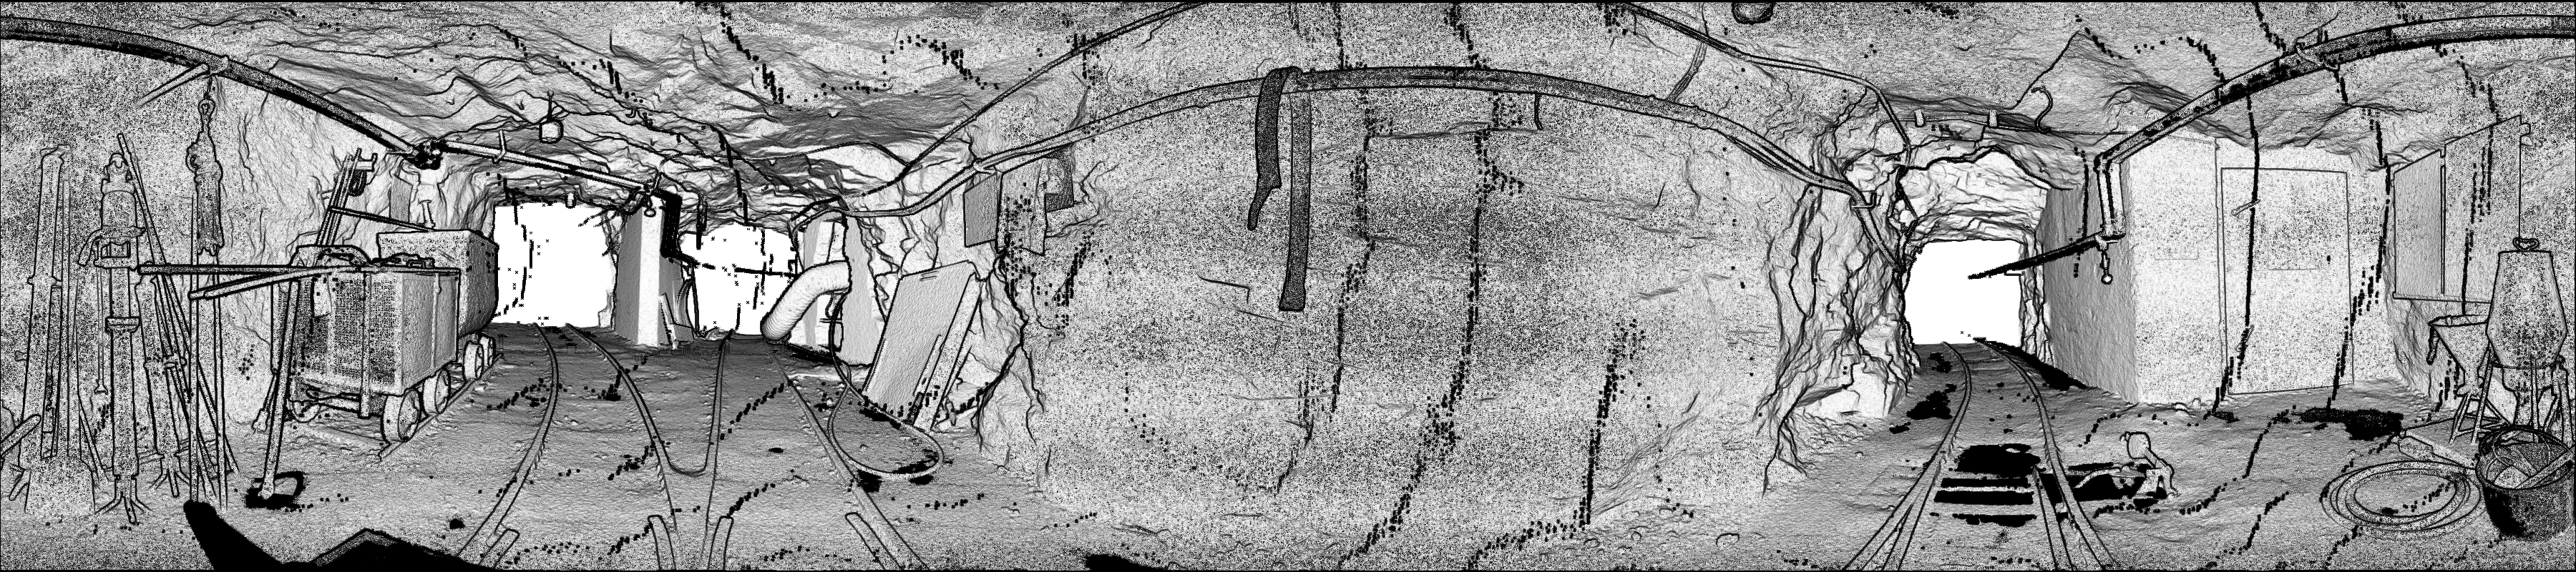
\includegraphics[width=1\linewidth]{chapter05/img/scans/flexion-0001.png}\\
    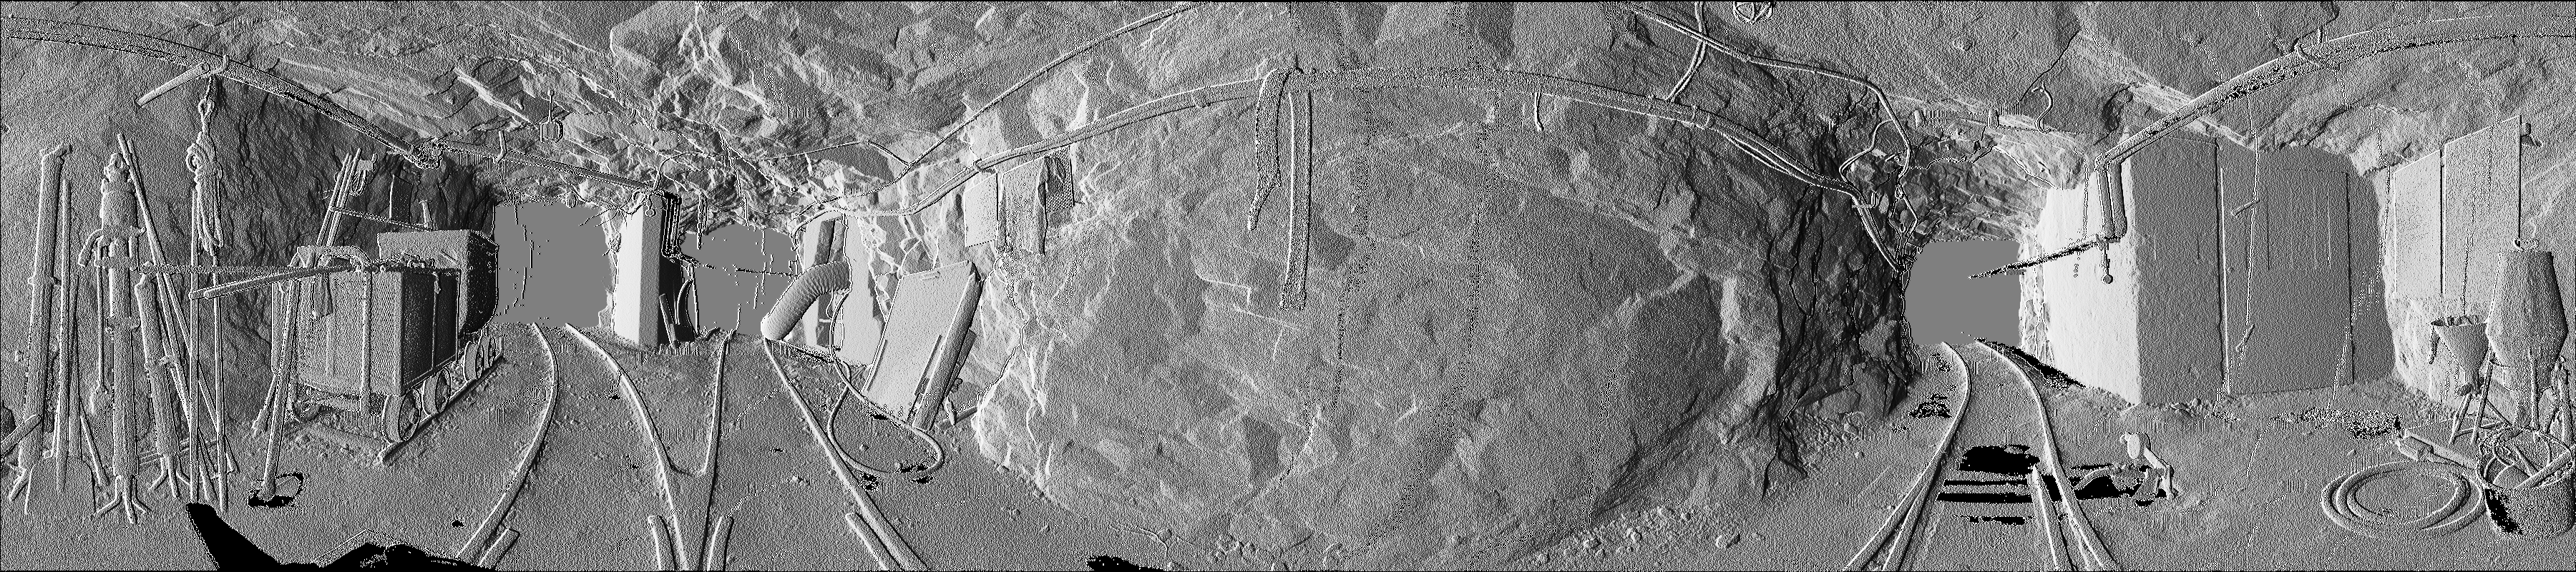
\includegraphics[width=1\linewidth]{chapter05/img/scans/bearing-0001.png}%
    }
    {\caption{The raw \acrshort{LIDAR} scans and their conversions.}\label{fig:scans}}
\end{floatrow}
\end{figure}

\begin{table}[H]
    {\renewcommand{\arraystretch}{1.3}%
    \setlength{\tabcolsep}{0.3em}%
    \begin{tabular}{ccccc}
    \toprule
    \null & \textbf{Synthetic} & \textbf{Lehrpfad} & \textbf{Office} & \textbf{Laserscan} \\
    \midrule
    \textbf{Camera Model} & pinhole & pinhole & pinhole & equirectangular \\
    \textbf{Number Images} & 211 & 734 & 57 & 6 \\
    \textbf{Distribution} & \ding{52} & \ding{52} & \ding{52} & \ding{52} \\
    \textbf{Keypoint Characteristics} & \ding{52} & \ding{52} & \ding{52} & \ding{52} \\
    \textbf{Matching Performance} & \ding{52} & \ding{52} & \ding{52} & \ding{56} \\
    \bottomrule
    \end{tabular}
    }
    \caption{An overview of all datasets and aspects of them were analyzed.}
\end{table}

\subsubsection{Synthetic City Scene Odometry}

The datasets evaluating the feature algorithms show the potential and performance of the common algorithms.
To demonstrate, that this performance translates into applicability the promising algorithms are used in a visual odometry scenario.
A synthetic dataset for city scenario, developed by Zhang et al.\cite{zhang_icra2016}, that provides a groundthruth trajectory is used for this purpose.
The in-house implementation of the visual odometry is very basic with the four following steps applied only on consecutive image.
First the feature are detected and their descriptors extracted, the descriptors are matched with OpenCV's RANSAC.
The essential matrix is computed in each RANSAC step and the consensus pose is used as relative pose.
Each feature algorithm is used with default configuration.
Both conditions imply that the result is not optimal and further optimizations would improve it further.

\newpage

\section{Results and Discussion}\label{sec:results}

First, the evaluation of the keypoint detector and descriptors is presented for \acrshort{sift}, \acrshort{surf}, \acrshort{orb} and \acrshort{akaze} with the focus on central results.
The out-of-the-box performance of each algorithm is compared with multiple custom processing configurations.
After a short conclusion of the feature performance \acrshort{sift} and \acrshort{akaze} are selected to compute a visual odometry on an unseen benchmark dataset.
Subsequently, the results are discussed.

\subsection{Algorithm Performance}

Each algorithm with own section, important is distribution, keypoint characteristics, descriptor distances

\subsubsection{Odometry}

\begin{figure}[H]
    \includegraphics[width=0.5\linewidth]{chapter06/odo/jonas_flexion_AKAZE.png}
    \caption{Flexion image with AKAZE as basis for odometry}
\end{figure}

\subsection{Keypoint-Detector discussion}

\begin{itemize}
    \item Stable Keypoints are important
    \item good Keypoint distribution
\end{itemize}

\subsection{Feature-Descriptor Discussion}

\begin{itemize}
    \item matching performance
    \item Computational Complexity
\end{itemize}

\subsection{Error Discussion}

The datasets are affected by different errors and simplifications, that are discussed in this section.
\emph{Synthetic} is a noise free dataset with very simple scene structure.
Findings and conclusion based on this dataset are only of principle nature but do not reflect real world performance.

The \emph{Mine} and \emph{Office} dataset are both gathered using the same Kinectv2 technology, but under different conditions and environments.
\emph{Mine}, an underground mining environment with partially wet walls, contains drastically more missing depth measurements.
For parts of the whole trajectory, it is very challenging to make out the basic shapes of the scene as a human.
The computer vision algorithms can not magically perform better at these places.
Parts of the scene are not within the measurement range, the walls and wide areas are not fully lit by the sensor's infrared \acrshort{led} or the light is absorbed by water.
Missing range measurements also occur in \emph{Office}, but the overall influence of bad conditions is not as high as in \emph{Mine}.

Another major consideration is the rectification of the depth images before being processed by the proposed pipeline.
The native resolution of the Kinectv2 depth sensor is 512$\times$424\,px\cite{wasenmuller_accv2016}, which is lower than the input depth images used for the feature image conversions.
This change in resolution is artifact of \acrshort{ROS}' image rectification, that maps each depth pixel to its matching color pixel.
The experiments show no qualitative difference of results between different image scales, but unrectified depth images experience distortion which will change the results at the image borders.
The sensors depth image is noticibly affected by smaller waves in the conversion images for stand images.
Their effect is considered small, because different filtering algorithms show only slight changes in the final result.
The much finer resolution of the \emph{Laserscan} dataset on the other hand showed that prior filtering with median blur can improve the quality of the final feature image drastically (Appendix~\ref{sec:laserscan_conversions}).

There are no errors expected from the implementation of the software as all components are thoroughly tested.
The usage of integers to store the range information on the other hand creates visible artifacts.
Their effect is neglectable because every feature algorithm employs some form of blurring and detail reduction.

\newpage

\section{Conclusion}\label{sec:conclusion}

This thesis evaluated the use of state-of-the-art computer vision feature detection and description algorithms to find salient points in a depth image.
Instead of direct application of the algorithm to the depth image, it is transformed into a derived image constructed from local geometric properties of the depth values.
The approach is introduced by Scaramuzza et al.\cite{scaramuzza_iros2007} with their \gls{bearing-angle-image} and the usage of \acrshort{surf} to detect keypoints on those by Lin et al.\cite{lin_easp2017}.
To overcome the \gls{bearing-angle-image}'s limitation, the lack of rotation invariance, this work proposed four additional feature image conversions.
Only the \gls{flexion-image} is judged as viable.
The performance of \acrshort{sift}, \acrshort{surf}, \acrshort{orb} and \acrshort{akaze} were evaluated for both the \gls{bearing-angle} and the \gls{flexion-image}.
Surprisingly, the evaluation showed that \acrshort{surf} lacks descriptive power to achieve good recognition performance.
\acrshort{orb}'s corner-based keypoint detector failed to produce stable keypoints.
\acrshort{sift} and \acrshort{akaze} were the only algorithms achieving acceptable detection and recognition performance.
The findings of this thesis --- the novel \gls{flexion-image} and its performance for \acrshort{sift} and \acrshort{akaze} --- may be the foundation for a descriptor for dense, structured pointcloud data, a problem not solved satisfactory yet.

The proposed conversion has been tested with a Kinectv2 depth sensor and the Riegl Z300 \acrshort{LIDAR} scanner.
Preprocessing the depth data with edge-preserving filtering was part of the evaluation and has proven to be useful for the Riegl Z300, but unnecessary for the Kinectv2 sensor.
Applying a median blur is enough for consistent smooth results and a more advanced bilateral filtering was not beneficial.

The implementation of the evaluation software and conversion code was done with state-of-the-art software engineering principles and is of high quality.
It can be used for follow up research and various binary artifacts are produced that run on any Linux system and can be compiled from source if required.

The proposed \gls{flexion-image} bridges the gap between pointcloud processing and classical computer vision algorithms.
Common processes, such as visual odometry, global localisation and maybe even optical flow algorithms should be evaluated.
The foundational insights on the descriptor performance of \acrshort{sift} and \acrshort{akaze} help to fine-tune heuristics, such as the maximum matching distance, for these tasks.
The feature image conversions implementations can be optimized by better \acrshort{SIMD} support and caching intermediate results like the spherical coordinates for pixels.
Each conversion is suited for \acrshort{GPGPU} computation and drastic speed-ups of their computations are expected.

New formulations for visual odometry and relative pose calculation become possible because the range value for each pixel is available.
This additional information reduces the required number of true correspondences to reconstruct the relative pose.
Investigating the viability of a new formulation for this problem and potential speed and efficiency gains seems to be the highest value research targets.
The classical \acrshort{icp} formulation relies on establishing explicit correspondences between points, too.
Using the \gls{flexion-image} and classical feature descriptors might result in a new variation of this algorithm.
Both problems are related and need further research.

\newpage

\begin{appendix}
    % \clearpage
    \renewcommand*{\thepage}{\thesection\arabic{page}}
    \renewcommand{\thetable}{\thesection\arabic{table}}
    \renewcommand{\thefigure}{\thesection\arabic{figure}}

    % \input{anhang/content}
    \newpage

    \section{Mathematical Derivation}
    \subsection{Bearing-Angle Formula}\label{sec:bearing_derivation}

This section provides the exact derivation of the \gls{bearing-angle} formula.
The literature on \gls{bearing-angle} disagrees on the formula and have mathematical errors.
The full chain of derivation and graphical presentations goal is to provide a trustworthy and checkable background for the provided formula.

\begin{figure}[H]
    

\tikzset{every picture/.style={line width=0.75pt}} %set default line width to 0.75pt        

\begin{tikzpicture}[x=0.75pt,y=0.75pt,yscale=-1,xscale=1]
%uncomment if require: \path (0,269); %set diagram left start at 0, and has height of 269

%Straight Lines [id:da6739847496898159] 
\draw  [dash pattern={on 0.84pt off 2.51pt}]  (122.83,126.01) -- (252.88,63) ;
%Shape: Arc [id:dp4878212457791631] 
\draw  [draw opacity=0] (240.62,97.61) .. controls (227.55,94.98) and (217.71,83.44) .. (217.71,69.6) .. controls (217.71,63.88) and (219.39,58.55) .. (222.28,54.08) -- (246.29,69.6) -- cycle ; \draw  [color={rgb, 255:red, 208; green, 2; blue, 27 }  ,draw opacity=1 ] (240.62,97.61) .. controls (227.55,94.98) and (217.71,83.44) .. (217.71,69.6) .. controls (217.71,63.88) and (219.39,58.55) .. (222.28,54.08) ;
%Shape: Arc [id:dp901574933751006] 
\draw  [draw opacity=0] (113.13,25.58) .. controls (112.48,40.91) and (102.88,53.93) .. (89.43,59.54) -- (74.58,23.92) -- cycle ; \draw  [color={rgb, 255:red, 74; green, 144; blue, 226 }  ,draw opacity=1 ] (113.13,25.58) .. controls (112.48,40.91) and (102.88,53.93) .. (89.43,59.54) ;
%Shape: Polygon [id:ds6190617836836185] 
\draw   (67.51,13.91) -- (255.81,63) -- (178.15,238.12) -- cycle ;
%Shape: Ellipse [id:dp4849771561113211] 
\draw  [fill={rgb, 255:red, 0; green, 0; blue, 0 }  ,fill opacity=1 ] (251.95,63) .. controls (251.95,61.38) and (253.26,60.07) .. (254.88,60.07) .. controls (256.5,60.07) and (257.81,61.38) .. (257.81,63) .. controls (257.81,64.62) and (256.5,65.93) .. (254.88,65.93) .. controls (253.26,65.93) and (251.95,64.62) .. (251.95,63) -- cycle ;
%Shape: Circle [id:dp8356396848663105] 
\draw  [fill={rgb, 255:red, 0; green, 0; blue, 0 }  ,fill opacity=1 ] (64.58,13.84) .. controls (64.58,12.22) and (65.89,10.91) .. (67.51,10.91) .. controls (69.13,10.91) and (70.44,12.22) .. (70.44,13.84) .. controls (70.44,15.46) and (69.13,16.77) .. (67.51,16.77) .. controls (65.89,16.77) and (64.58,15.46) .. (64.58,13.84) -- cycle ;
%Shape: Arc [id:dp8012007227541399] 
\draw  [draw opacity=0] (157.23,196.86) .. controls (163.51,193.67) and (170.62,191.87) .. (178.15,191.87) .. controls (184.79,191.87) and (191.12,193.27) .. (196.83,195.8) -- (178.15,238.12) -- cycle ; \draw   (157.23,196.86) .. controls (163.51,193.67) and (170.62,191.87) .. (178.15,191.87) .. controls (184.79,191.87) and (191.12,193.27) .. (196.83,195.8) ;
%Shape: Right Angle [id:dp07010543377164635] 
\draw   (116.98,113.65) -- (129.04,107.95) -- (134.88,120.31) ;

% Text Node
\draw (161.42,20.19) node [anchor=north west][inner sep=0.75pt]   [align=left] {$\displaystyle a$};
% Text Node
\draw (159.22,87.59) node [anchor=north west][inner sep=0.75pt]   [align=left] {$\displaystyle h$};
% Text Node
\draw (230.37,126.44) node [anchor=north west][inner sep=0.75pt]   [align=left] {$\displaystyle d_{i}$};
% Text Node
\draw (93.81,128.37) node [anchor=north west][inner sep=0.75pt]   [align=left] {$\displaystyle d_{i-1}$};
% Text Node
\draw (168.08,197.65) node [anchor=north west][inner sep=0.75pt]   [align=left] {$\displaystyle d\varphi $};
% Text Node
\draw (230.1,71.96) node [anchor=north west][inner sep=0.75pt]  [color={rgb, 255:red, 208; green, 2; blue, 27 }  ,opacity=1 ] [align=left] {$\displaystyle \beta $};
% Text Node
\draw (87.69,32.2) node [anchor=north west][inner sep=0.75pt]  [color={rgb, 255:red, 74; green, 144; blue, 226 }  ,opacity=1 ] [align=left] {$\displaystyle \gamma $};
% Text Node
\draw (101.34,65.61) node [anchor=north west][inner sep=0.75pt]   [align=left] {$\displaystyle b$};
% Text Node
\draw (144.57,151.34) node [anchor=north west][inner sep=0.75pt]   [align=left] {$\displaystyle c$};
% Text Node
\draw (169.08,242.2) node [anchor=north west][inner sep=0.75pt]   [align=left] {$\displaystyle \mathbf{C}$};
% Text Node
\draw (261,53.76) node [anchor=north west][inner sep=0.75pt]   [align=left] {$\displaystyle \mathbf{P}_{i}$};
% Text Node
\draw (28.06,8.4) node [anchor=north west][inner sep=0.75pt]   [align=left] {$\displaystyle \mathbf{P}_{i-1}$};


\end{tikzpicture}


    \caption[Derivation of Bearing-Angle with all Support Variables]{Deriving the bearing angle requires additional support variables that are introduced with this figure. Using fundamental trigonometry allows derivation of the formula.}\label{fig:bearing-derivation}
\end{figure}

The cosine theorem holds true for all triangles and is the central equality for the derivation.
\begin{equation}
\begin{aligned}
    \text{Ansatz:} \\
    d_{i-1}^2 &= d_i^2 + a^2 - 2 d_i a \cos \beta \qquad \text{(Cosine Theorem)} \\
\end{aligned}
\end{equation}
Introducing supporting variables at the positions given in figure~\ref{fig:bearing-derivation} allows substiting the missing quantity $a$.
\begin{equation*}
\begin{aligned}
    h &= d_i \sin d\varphi \\
    c &= d_i \cos d\varphi \\
    b &= d_{i-1} - d_i \cos d\varphi \\
    a^2 &= h^2 + b^2 \\
    a^2 &= \mathunderline{darkgreen}{(d_i \sin d\varphi)^2} + \mathunderline{plotblue}{(d_{i-1} - d_i \cos d\varphi)^2} \\
    a^2 &= \mathunderline{darkgreen}{\mathunderline{darkred}{d_i^2 \sin^2 d\varphi}} +
           \mathunderline{plotblue}{%
             \mathunderline{plotorange}{d_{i-1}^2 - 2 d_{i-1} d_i \cos d\varphi} +
             \mathunderline{darkred}{d_i^2 \cos^2 d\varphi}
           } \\
    a^2 &= \mathunderline{darkred}{d_{i-1}^2 \sin^2 d\varphi + d_{i-i}^2 \cos^2 d\varphi} +
           \mathunderline{plotorange}{d_{i-1}^2 -2 d_{i-1} d_i \cos d\varphi} \\
    a^2 &= \mathunderline{darkred}{d_i^2} +
           \mathunderline{plotorange}{d_{i-1}^2 - 2 d_{i-1} d_i \cos d\varphi} \\
\end{aligned}
\end{equation*}
For $a$ holds the condition $a > 0$ for all values, because the constraints $d_i > 0$, $d_{i-1} > 0$ and $0 < d\varphi < \pi$ result from the properties of depth sensors.

The variable $a$ is now substituted in the ansatz.
Consequent simplification of the equations yields the final formula for the bearing angle.
\begin{equation*}
\begin{aligned}
    d_{i-1}^2 &= d_i^2 + a^2 - 2 d_i a \cos \beta \\
    \mathunderline{plotblue}{d_{i-1}^2} &= \mathunderline{darkred}{d_i^2} +
    \mathunderline{darkred}{d_i^2} + \mathunderline{plotblue}{d_{i-1}^2} - 2 d_{i-1} d_i \cos d\varphi
    - 2 d_i \sqrt{d_i^2 + d_{i-1}^2 -2 d_{i-1} d_i \cos d\varphi} \cos \beta \\
    \mathunderline{plotblue}{0} &= \mathunderline{darkgreen}{2} \mathunderline{darkred}{d_i^2} +
                                   \mathunderline{plotblue}{0} -
                                   \mathunderline{darkgreen}{2} \mathunderline{darkred}{d_{i-1}} d_i \cos d\varphi
                                   - \mathunderline{darkgreen}{2} \mathunderline{darkred}{d_i} \sqrt{d_i^2 + d_{i-1}^2 -2 d_{i-1} d_i \cos d\varphi} \cos \beta \\
   0 &= \mathunderline{darkred}{d_i^2} - \mathunderline{darkred}{d_{i}} d_{i-1} \cos d\varphi
       - \mathunderline{darkred}{d_i} \sqrt{d_i^2 + d_{i-1}^2 -2 d_{i-1} d_i \cos d\varphi} \cos \beta \\
   0 &= \mathunderline{darkred}{d_i} - \mathunderline{darkred}{1} d_{i-1} \cos d\varphi
       - \mathunderline{darkred}{1} \sqrt{d_i^2 + d_{i-1}^2 -2 d_{i-1} d_i \cos d\varphi} \cos \beta \\
   \cos \beta &= \frac{d_i - d_{i-1} \cos d\varphi}{\sqrt{d_i^2 + d_{i-1}^2 -2 d_{i-1} d_i \cos d\varphi}} \\
   \beta &= \arccos \frac{d_i - d_{i-1} \cos d\varphi}{\sqrt{d_i^2 + d_{i-1}^2 -2 d_{i-1} d_i \cos d\varphi}} \\
\end{aligned}
\end{equation*}

% vim: set nocindent nosmartindent

    \newpage

    \section{Converted Images for Datasets}
    {\setlength{\abovecaptionskip}{-20pt}%
     \setlength{\belowcaptionskip}{-30pt}%
     \setlength{\floatsep}{1pt plus 1pt minus 1pt}%
     \setlength{\textfloatsep}{1pt plus 1.0pt minus 2.0pt}
     \setlength{\intextsep}{1pt plus 1.0pt minus 2.0pt}
    \subsection{Synthetic}\label{sec:synthetic_conversions}
\begin{figure}[H]
    \includegraphics[width=0.25\linewidth]{chapter06/results/conv_images/synthetic/flexion/raw/0040.png}%
    \includegraphics[width=0.25\linewidth]{chapter06/results/conv_images/synthetic/flexion/raw/0080.png}%
    \includegraphics[width=0.25\linewidth]{chapter06/results/conv_images/synthetic/flexion/raw/0120.png}%
    \includegraphics[width=0.25\linewidth]{chapter06/results/conv_images/synthetic/flexion/raw/0160.png}\\
    \includegraphics[width=0.25\linewidth]{chapter06/results/conv_images/synthetic/bearing/raw/0040.png}%
    \includegraphics[width=0.25\linewidth]{chapter06/results/conv_images/synthetic/bearing/raw/0080.png}%
    \includegraphics[width=0.25\linewidth]{chapter06/results/conv_images/synthetic/bearing/raw/0120.png}%
    \includegraphics[width=0.25\linewidth]{chapter06/results/conv_images/synthetic/bearing/raw/0160.png}%
    \caption{The synthetic scene's conversion to \glspl{flexion-image} and \glspl{bearing-angle-image}. No filtering is applied, because the range data has no error.}
\end{figure}

    \subsection{Office}\label{sec:office_conversions}
\begin{figure}[H]
    \includegraphics[width=0.25\linewidth]{chapter06/results/conv_images/office/flexion/raw/0000.png}%
    \includegraphics[width=0.25\linewidth]{chapter06/results/conv_images/office/flexion/raw/0014.png}%
    \includegraphics[width=0.25\linewidth]{chapter06/results/conv_images/office/flexion/raw/0028.png}%
    \includegraphics[width=0.25\linewidth]{chapter06/results/conv_images/office/flexion/raw/0042.png}\\
    \includegraphics[width=0.25\linewidth]{chapter06/results/conv_images/office/bearing/raw/0000.png}%
    \includegraphics[width=0.25\linewidth]{chapter06/results/conv_images/office/bearing/raw/0014.png}%
    \includegraphics[width=0.25\linewidth]{chapter06/results/conv_images/office/bearing/raw/0028.png}%
    \includegraphics[width=0.25\linewidth]{chapter06/results/conv_images/office/bearing/raw/0042.png}\\
    \caption{Example \glspl{flexion-image} and \glspl{bearing-angle-image} of the Office dataset without any filtering.}
\end{figure}
\begin{figure}[H]
    \includegraphics[width=0.25\linewidth]{chapter06/results/conv_images/office/flexion/mb/0014.png}%
    \includegraphics[width=0.25\linewidth]{chapter06/results/conv_images/office/flexion/mb/0028.png}%
    \includegraphics[width=0.25\linewidth]{chapter06/results/conv_images/office/bearing/mb/0014.png}%
    \includegraphics[width=0.25\linewidth]{chapter06/results/conv_images/office/bearing/mb/0028.png}%
    \caption{Filtering the range data with median blur before conversion.}
\end{figure}
\begin{figure}[H]
    \includegraphics[width=0.25\linewidth]{chapter06/results/conv_images/office/flexion/bl/0014.png}%
    \includegraphics[width=0.25\linewidth]{chapter06/results/conv_images/office/flexion/bl/0028.png}%
    \includegraphics[width=0.25\linewidth]{chapter06/results/conv_images/office/bearing/bl/0014.png}%
    \includegraphics[width=0.25\linewidth]{chapter06/results/conv_images/office/bearing/bl/0028.png}%
    \caption{Filtering the range data with a bilateral filter before conversion.}
\end{figure}

    \subsection{Laserscan}\label{sec:laserscan_conversions}
\begin{figure}[H]
    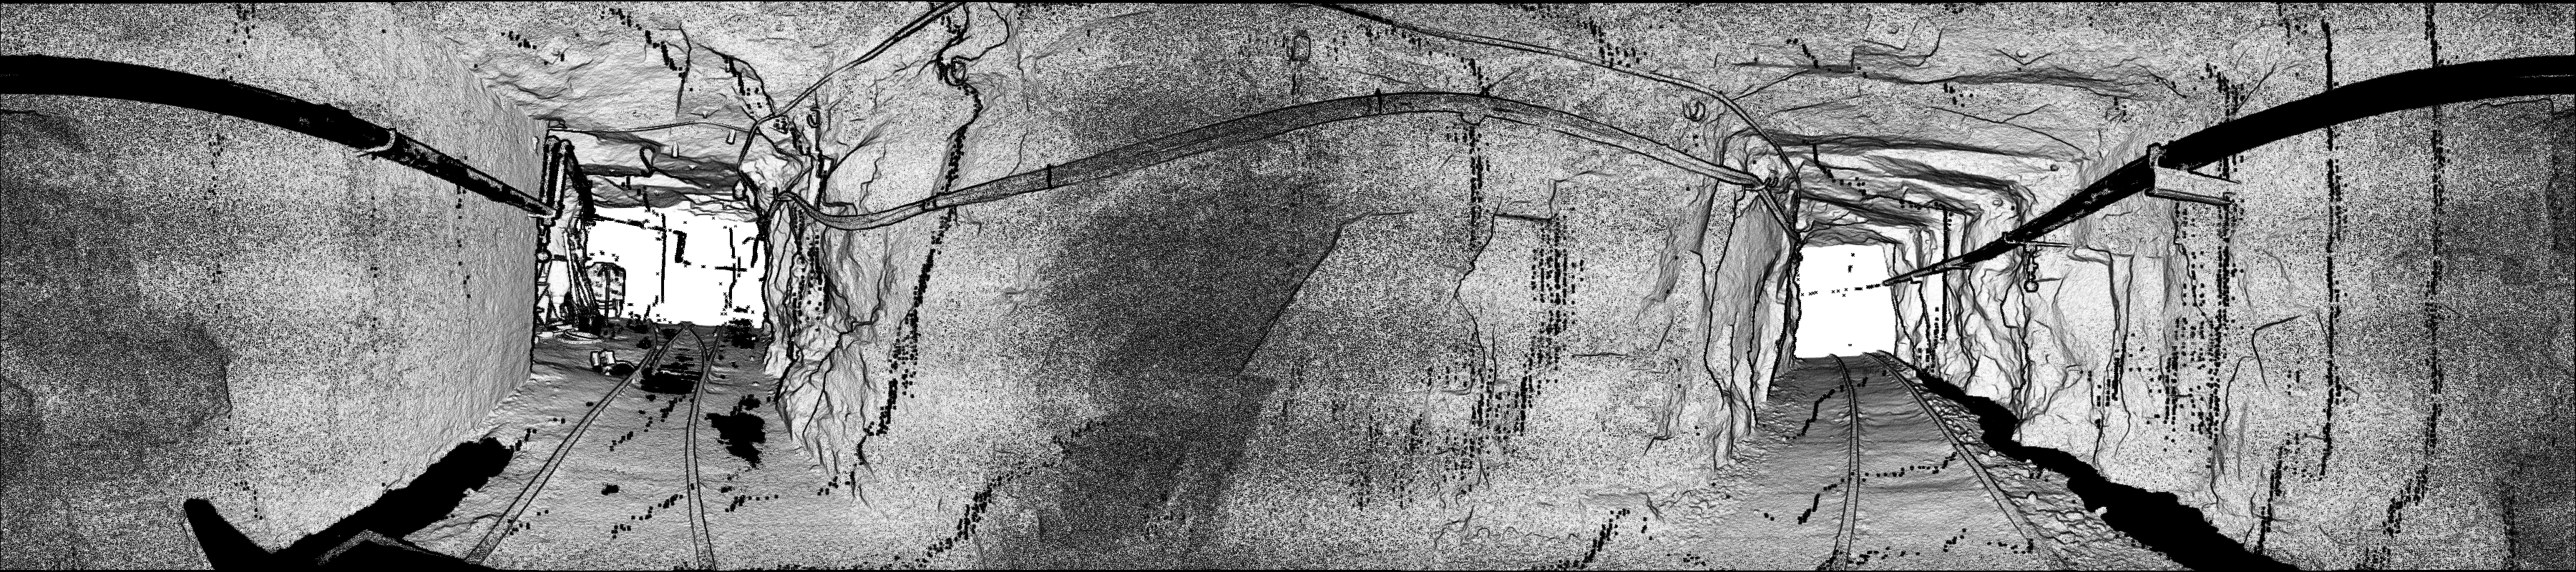
\includegraphics[width=1.0\linewidth]{chapter06/results/conv_images/laserscan/flexion/raw/0000.png}\\
    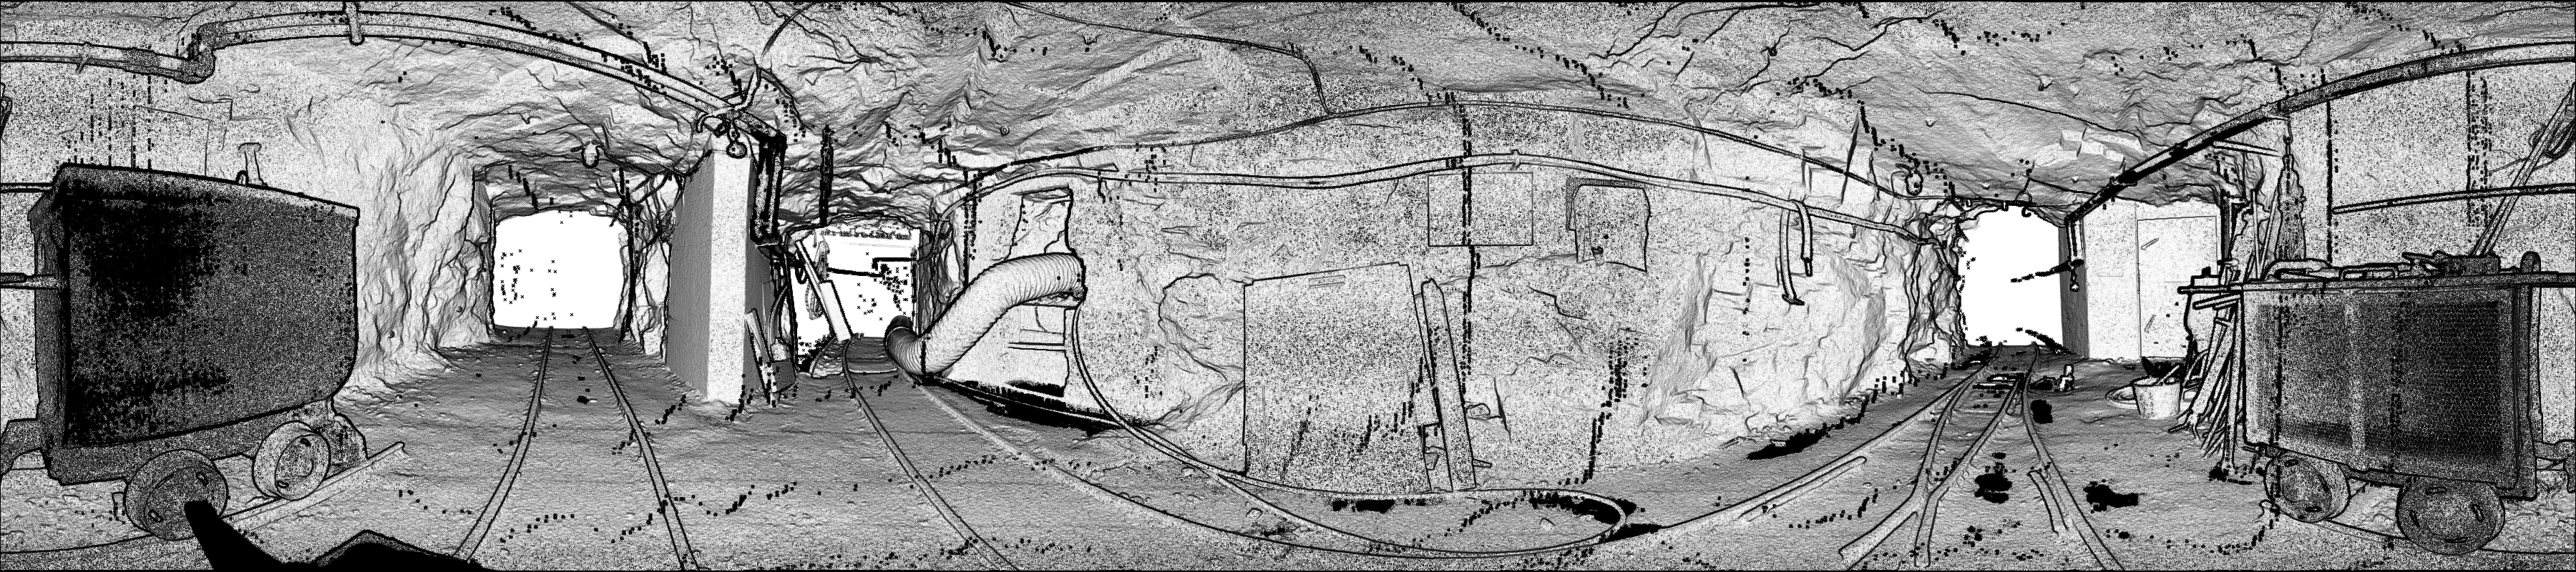
\includegraphics[width=1.0\linewidth]{chapter06/results/conv_images/laserscan/flexion/raw/0002.png}\\
    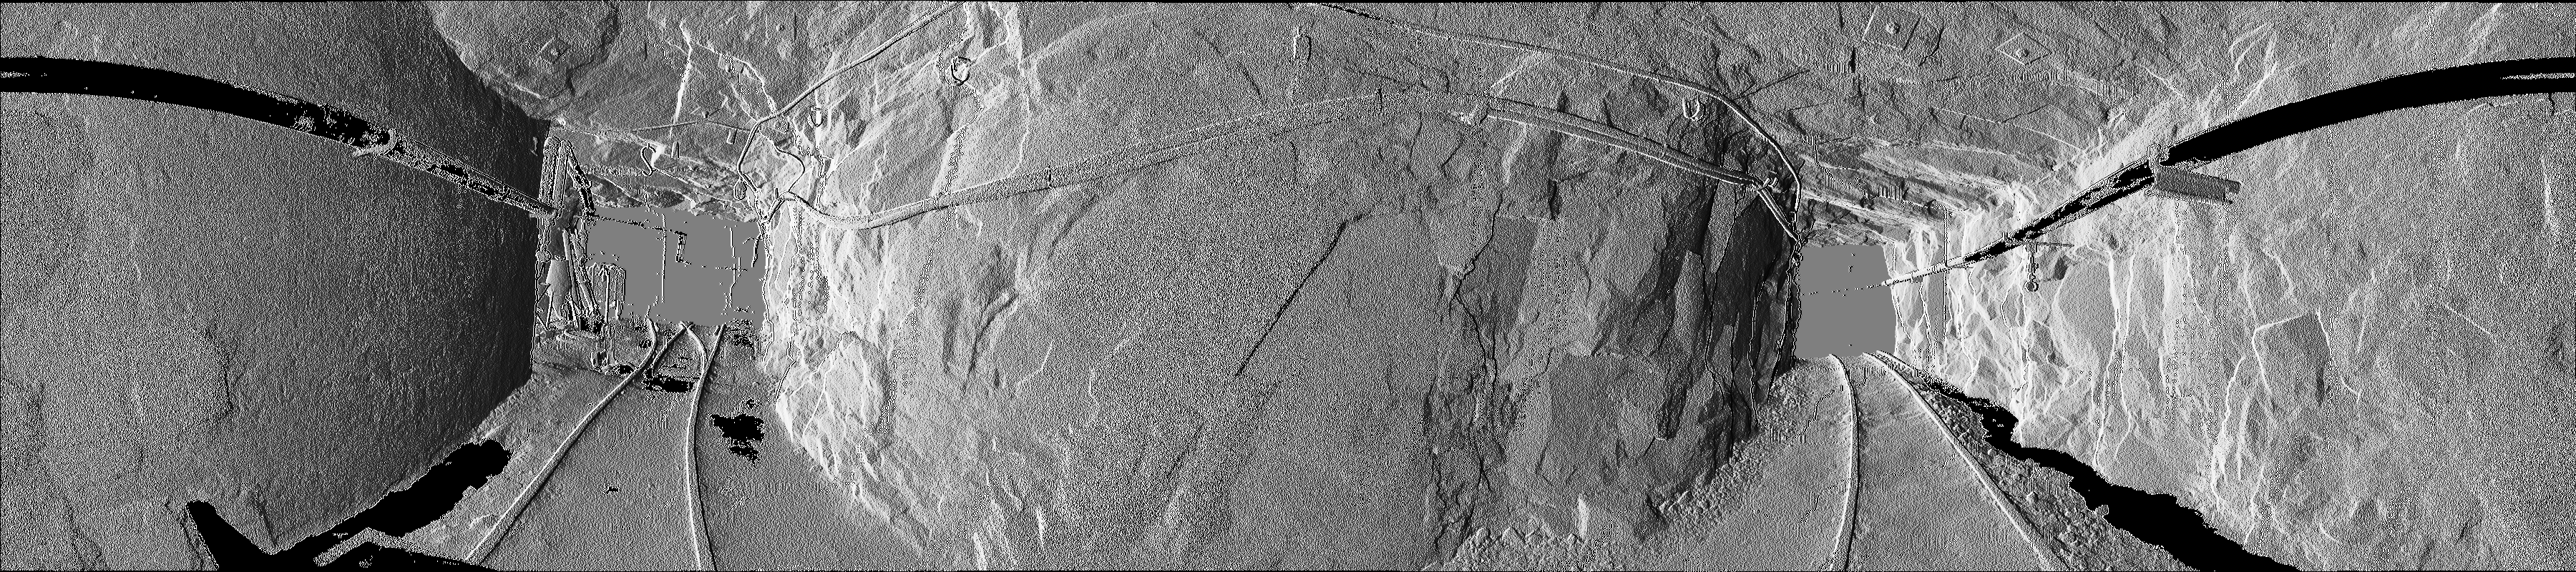
\includegraphics[width=1.0\linewidth]{chapter06/results/conv_images/laserscan/bearing/raw/0000.png}\\
    \includegraphics[width=1.0\linewidth]{chapter06/results/conv_images/laserscan/bearing/raw/0002.png}
    \caption[Examples of the \emph{Laserscan} feature image conversions]{Example \glspl{flexion-image} and \glspl{bearing-angle-image} of the Laserscan dataset without any filtering.}
\end{figure}
\begin{figure}[H]
    \includegraphics[width=1.0\linewidth]{chapter06/results/conv_images/laserscan/flexion/mb/0002.png}\\
    \includegraphics[width=1.0\linewidth]{chapter06/results/conv_images/laserscan/bearing/mb/0002.png}%
    \caption{Effect of median blur filtering on the \emph{Laserscan} data.}
\end{figure}
\begin{figure}[H]
    \includegraphics[width=1.0\linewidth]{chapter06/results/conv_images/laserscan/flexion/bl/0002.png}\\
    \includegraphics[width=1.0\linewidth]{chapter06/results/conv_images/laserscan/bearing/bl/0002.png}%
    \caption{Effect of bilateral filtering on the \emph{Laserscan} data.}
\end{figure}

    \subsection{Lehrpfad}\label{sec:lehrpfad_conversions}
\begin{figure}[H]
    \includegraphics[width=0.25\linewidth]{chapter06/results/conv_images/lehrpfad/flexion/raw/0000.png}%
    \includegraphics[width=0.25\linewidth]{chapter06/results/conv_images/lehrpfad/flexion/raw/0090.png}%
    \includegraphics[width=0.25\linewidth]{chapter06/results/conv_images/lehrpfad/flexion/raw/0180.png}%
    \includegraphics[width=0.25\linewidth]{chapter06/results/conv_images/lehrpfad/flexion/raw/0270.png}\\
    \includegraphics[width=0.25\linewidth]{chapter06/results/conv_images/lehrpfad/flexion/raw/0360.png}%
    \includegraphics[width=0.25\linewidth]{chapter06/results/conv_images/lehrpfad/flexion/raw/0450.png}%
    \includegraphics[width=0.25\linewidth]{chapter06/results/conv_images/lehrpfad/flexion/raw/0540.png}%
    \includegraphics[width=0.25\linewidth]{chapter06/results/conv_images/lehrpfad/flexion/raw/0630.png}\\
    \includegraphics[width=0.25\linewidth]{chapter06/results/conv_images/lehrpfad/bearing/raw/0000.png}%
    \includegraphics[width=0.25\linewidth]{chapter06/results/conv_images/lehrpfad/bearing/raw/0090.png}%
    \includegraphics[width=0.25\linewidth]{chapter06/results/conv_images/lehrpfad/bearing/raw/0180.png}%
    \includegraphics[width=0.25\linewidth]{chapter06/results/conv_images/lehrpfad/bearing/raw/0270.png}\\
    \includegraphics[width=0.25\linewidth]{chapter06/results/conv_images/lehrpfad/bearing/raw/0360.png}%
    \includegraphics[width=0.25\linewidth]{chapter06/results/conv_images/lehrpfad/bearing/raw/0450.png}%
    \includegraphics[width=0.25\linewidth]{chapter06/results/conv_images/lehrpfad/bearing/raw/0540.png}%
    \includegraphics[width=0.25\linewidth]{chapter06/results/conv_images/lehrpfad/bearing/raw/0630.png}%
    \caption[Examples of the \emph{Lehrpfad} feature image conversions]{Example \glspl{flexion-image} and \glspl{bearing-angle-image} of the \emph{Lehrpfad} dataset without any filtering.}
\end{figure}
\begin{figure}[H]
    \includegraphics[width=0.25\linewidth]{chapter06/results/conv_images/lehrpfad/flexion/mb/0000.png}%
    \includegraphics[width=0.25\linewidth]{chapter06/results/conv_images/lehrpfad/flexion/mb/0360.png}%
    \includegraphics[width=0.25\linewidth]{chapter06/results/conv_images/lehrpfad/bearing/mb/0000.png}%
    \includegraphics[width=0.25\linewidth]{chapter06/results/conv_images/lehrpfad/bearing/mb/0360.png}%
    \caption{Effect of median blur filtering on the \emph{Lehrpfad} data.}
\end{figure}
\begin{figure}[H]
    \includegraphics[width=0.25\linewidth]{chapter06/results/conv_images/lehrpfad/flexion/bl/0000.png}%
    \includegraphics[width=0.25\linewidth]{chapter06/results/conv_images/lehrpfad/flexion/bl/0360.png}%
    \includegraphics[width=0.25\linewidth]{chapter06/results/conv_images/lehrpfad/bearing/bl/0000.png}%
    \includegraphics[width=0.25\linewidth]{chapter06/results/conv_images/lehrpfad/bearing/bl/0360.png}%
    \caption{Effect of bilateral filtering on the \emph{Lehrpfad} data.}
\end{figure}

    }
    \newpage

    \section{Keypoints and Backprojections for \acrshort{sift} and \acrshort{akaze}}
    The plots in this section show the combined keypoint and matching performance.
    Green points are a identified true positives and purple points false negative, making up the total correspondences.
    Orange lines connect false positives.
    \subsection{\acrshort{sift}}\label{sec:backprojection_sift}
\begin{figure}[H]
    \includegraphics[width=0.25\linewidth]{chapter06/results/SIFT/backprojections/lehrpfad/backprojected-0090.png}%
    \includegraphics[width=0.25\linewidth]{chapter06/results/SIFT/backprojections/lehrpfad/backprojected-0180.png}%
    \includegraphics[width=0.25\linewidth]{chapter06/results/SIFT/backprojections/lehrpfad/backprojected-0360.png}%
    \includegraphics[width=0.25\linewidth]{chapter06/results/SIFT/backprojections/lehrpfad/backprojected-0631.png}\\
    \includegraphics[width=0.25\linewidth]{chapter06/results/SIFT/backprojections/office/backprojected-0001.png}%
    \includegraphics[width=0.25\linewidth]{chapter06/results/SIFT/backprojections/office/backprojected-0014.png}%
    \includegraphics[width=0.25\linewidth]{chapter06/results/SIFT/backprojections/office/backprojected-0028.png}%
    \includegraphics[width=0.25\linewidth]{chapter06/results/SIFT/backprojections/office/backprojected-0042.png}\\
    \includegraphics[width=0.25\linewidth]{chapter06/results/SIFT/backprojections/synthetic/backprojected-0040.png}%
    \includegraphics[width=0.25\linewidth]{chapter06/results/SIFT/backprojections/synthetic/backprojected-0080.png}%
    \includegraphics[width=0.25\linewidth]{chapter06/results/SIFT/backprojections/synthetic/backprojected-0120.png}%
    \includegraphics[width=0.25\linewidth]{chapter06/results/SIFT/backprojections/synthetic/backprojected-0160.png}\\
    \includegraphics[width=1.0\linewidth]{chapter06/results/SIFT/backprojections/laserscan/keypoints-0000.png}\\
    \includegraphics[width=1.0\linewidth]{chapter06/results/SIFT/backprojections/laserscan/keypoints-0002.png}\\
    \caption[\acrshort{sift} backprojections and keypoints]{\acrshort{sift} backprojections for \texttt{raw/default} and keypoints of \texttt{median-blur/default} for \emph{Laserscan}}
\end{figure}

    \subsection{\acrshort{akaze}}\label{sec:backprojection_akaze}
\begin{figure}[H]
    \includegraphics[width=0.25\linewidth]{chapter06/results/AKAZE/backprojections/lehrpfad/backprojected-0090.png}%
    \includegraphics[width=0.25\linewidth]{chapter06/results/AKAZE/backprojections/lehrpfad/backprojected-0180.png}%
    \includegraphics[width=0.25\linewidth]{chapter06/results/AKAZE/backprojections/lehrpfad/backprojected-0360.png}%
    \includegraphics[width=0.25\linewidth]{chapter06/results/AKAZE/backprojections/lehrpfad/backprojected-0631.png}\\
    \includegraphics[width=0.25\linewidth]{chapter06/results/AKAZE/backprojections/office/backprojected-0001.png}%
    \includegraphics[width=0.25\linewidth]{chapter06/results/AKAZE/backprojections/office/backprojected-0014.png}%
    \includegraphics[width=0.25\linewidth]{chapter06/results/AKAZE/backprojections/office/backprojected-0028.png}%
    \includegraphics[width=0.25\linewidth]{chapter06/results/AKAZE/backprojections/office/backprojected-0042.png}\\
    \includegraphics[width=0.25\linewidth]{chapter06/results/AKAZE/backprojections/synthetic/backprojected-0040.png}%
    \includegraphics[width=0.25\linewidth]{chapter06/results/AKAZE/backprojections/synthetic/backprojected-0080.png}%
    \includegraphics[width=0.25\linewidth]{chapter06/results/AKAZE/backprojections/synthetic/backprojected-0120.png}%
    \includegraphics[width=0.25\linewidth]{chapter06/results/AKAZE/backprojections/synthetic/backprojected-0160.png}\\
    \includegraphics[width=1.0\linewidth]{chapter06/results/AKAZE/backprojections/laserscan/keypoints-0000.png}\\
    \includegraphics[width=1.0\linewidth]{chapter06/results/AKAZE/backprojections/laserscan/keypoints-0002.png}\\
    \caption[\acrshort{akaze} backprojections and keypoints]{\acrshort{akaze} backprojections for \texttt{raw/best-only} and keypoints of \texttt{median-blur/best-only} for \emph{Laserscan}}
\end{figure}

    \newpage

    \section{In-Depth Statistics for Datasets}
    \subsection{\acrshort{sift}}\label{sec:sift_stats}
\begin{figure}[H]
\begin{subfigure}[t]{0.45\linewidth}
    \includegraphics[width=\linewidth]{chapter06/results/SIFT/flexion/size.pdf}%
    \caption{\gls{flexion-image}}
\end{subfigure}\quad
\begin{subfigure}[t]{0.45\linewidth}
    \includegraphics[width=\linewidth]{chapter06/results/SIFT/bearing/size.pdf}
    \caption{\gls{bearing-angle-image}}
\end{subfigure}\\
\begin{subfigure}[t]{0.45\linewidth}
    \includegraphics[width=\linewidth]{chapter06/results/SIFT/flexion/response.pdf}%
    \caption{\gls{flexion-image}}
\end{subfigure}\quad
\begin{subfigure}[t]{0.45\linewidth}
    \includegraphics[width=\linewidth]{chapter06/results/SIFT/bearing/response.pdf}
    \caption{\gls{bearing-angle-image}}
\end{subfigure}
    \caption{Overview of keypoint sizes and responses for the \acrshort{sift} detector.}
\end{figure}
\begin{figure}[H]
    \includegraphics[width=\linewidth]{chapter06/results/SIFT/flexion/distribution.pdf}\\
    \includegraphics[width=\linewidth]{chapter06/results/SIFT/bearing/distribution.pdf}%
    \caption{Keypoint distribution for the \acrshort{sift} detector.}\label{fig:sift_kp_distribution}
\end{figure}

    \subsection{\acrshort{surf}}\label{sec:surf_stats}
\begin{figure}[H]
\begin{subfigure}[t]{0.45\linewidth}
    \includegraphics[width=\linewidth]{chapter06/results/SURF/flexion/size.pdf}%
    \caption{Flexion Image Keypoint Sizes}
\end{subfigure}\quad
\begin{subfigure}[t]{0.45\linewidth}
    \includegraphics[width=\linewidth]{chapter06/results/SURF/bearing/size.pdf}
    \caption{Bearing-Angle Keypoint Sizes}
\end{subfigure}\\
\begin{subfigure}[t]{0.45\linewidth}
    \includegraphics[width=\linewidth]{chapter06/results/SURF/flexion/response.pdf}%
    \caption{Flexion Image Keypoint Responses}
\end{subfigure}\quad
\begin{subfigure}[t]{0.45\linewidth}
    \includegraphics[width=\linewidth]{chapter06/results/SURF/bearing/response.pdf}
    \caption{Bearing-Angle Keypoint Responses}
\end{subfigure}
    \caption{Comparing Keypoint Sizes and Responses}
\end{figure}
\begin{figure}[H]
    \includegraphics[width=\linewidth]{chapter06/results/SURF/flexion/distribution.pdf}\\
    \includegraphics[width=\linewidth]{chapter06/results/SURF/bearing/distribution.pdf}%
    \caption{Keypoint Distribution for Flexion and Bearing.}
\end{figure}

    \subsection{\acrshort{orb}}\label{sec:orb_stats}
\begin{figure}[H]
\begin{subfigure}[t]{0.45\linewidth}
    \includegraphics[width=\linewidth]{chapter06/results/ORB/flexion/size.pdf}%
    \caption{Flexion Image Keypoint Sizes}
\end{subfigure}\quad
\begin{subfigure}[t]{0.45\linewidth}
    \includegraphics[width=\linewidth]{chapter06/results/ORB/bearing/size.pdf}
    \caption{Bearing-Angle Keypoint Sizes}
\end{subfigure}
    \caption{Comparing Keypoint Sizes}
\end{figure}
\begin{figure}[H]
\begin{subfigure}[t]{0.45\linewidth}
    \includegraphics[width=\linewidth]{chapter06/results/ORB/flexion/response.pdf}%
    \caption{Flexion Image Keypoint Responses}
\end{subfigure}\quad
\begin{subfigure}[t]{0.45\linewidth}
    \includegraphics[width=\linewidth]{chapter06/results/ORB/bearing/response.pdf}
    \caption{Bearing-Angle Keypoint Responses}
\end{subfigure}
    \caption{Comparing Keypoint Responses}
\end{figure}
\begin{figure}[H]
    \includegraphics[width=\linewidth]{chapter06/results/ORB/flexion/distribution.pdf}\\
    \includegraphics[width=\linewidth]{chapter06/results/ORB/bearing/distribution.pdf}%
    \caption{Keypoint Distribution for Flexion and Bearing.}
\end{figure}

    \subsection{\acrshort{akaze}}\label{sec:akaze_stats}
\begin{figure}[H]
\begin{subfigure}[t]{0.45\linewidth}
    \includegraphics[width=\linewidth]{chapter06/results/AKAZE/flexion/size.pdf}%
    \caption{\gls{flexion-image}}
\end{subfigure}\quad
\begin{subfigure}[t]{0.45\linewidth}
    \includegraphics[width=\linewidth]{chapter06/results/AKAZE/bearing/size.pdf}
    \caption{\gls{bearing-angle-image}}
\end{subfigure}
\begin{subfigure}[t]{0.45\linewidth}
    \includegraphics[width=\linewidth]{chapter06/results/AKAZE/flexion/response.pdf}%
    \caption{\gls{flexion-image}}
\end{subfigure}\quad
\begin{subfigure}[t]{0.45\linewidth}
    \includegraphics[width=\linewidth]{chapter06/results/AKAZE/bearing/response.pdf}
    \caption{\gls{bearing-angle-image}}
\end{subfigure}
    \caption{Overview of keypoint sizes and responses for the \acrshort{akaze} detector.}
\end{figure}
\begin{figure}[H]
    \includegraphics[width=\linewidth]{chapter06/results/AKAZE/flexion/distribution.pdf}\\
    \includegraphics[width=\linewidth]{chapter06/results/AKAZE/bearing/distribution.pdf}%
    \caption{Keypoint distribution for the \acrshort{akaze} detector.}
\end{figure}

    \newpage

    \addcontentsline{toc}{section}{References}
    \bibliographystyle{IEEEtran}
    \bibliography{references}

    \newpage
    \addcontentsline{toc}{section}{\listtablename}\listoftables

    \newpage
    \addcontentsline{toc}{section}{\listfigurename}\listoffigures

    \newpage
    %\renewcommand{\indexname}{Stichwortverzeichnis}
    %\addcontentsline{toc}{section}{Stichwortverzeichnis}
    % \printindex
\end{appendix}
\end{document}
